%                                     MMMMMMMMM                                         
%                                                                             
%  MMO    MM   MMMMMM  MMMMMMM   MM    MMMMMMMM   MMD   MM  MMMMMMM MMMMMMM   
%  MMM   MMM   MM        MM     ?MMM              MMM$  MM  MM         MM     
%  MMMM 7MMM   MM        MM     MM8M    MMMMMMM   MMMMD MM  MM         MM     
%  MM MMMMMM   MMMMMM    MM    MM  MM             MM MMDMM  MMMMMM     MM     
%  MM  MM MM   MM        MM    MMMMMM             MM  MMMM  MM         MM     
%  MM     MM   MMMMMM    MM   MM    MM            MM   MMM  MMMMMMM    MM
%
%
%            - META-NET Language Whitepaper | Icelandic paper -

\documentclass[]{../../metanetpaper}

%\usepackage{booktabs}
%\usepackage{longtable}
%\usepackage{tabulary}
%\usepackage{tabularx}
%\usepackage{rotating}
%\usepackage{makecell}
%\usepackage{multirow}
%\usepackage{colortbl}
%\usepackage{polyglossia}
%\usepackage{multicol,framed,lipsum}
%\setotherlanguages{icelandic,english}
\usepackage[icelandic, english]{babel}

%!TEX TS-program = xelatex
\RequireXeTeX %Force XeTeX check

\title{Íslensk tunga á stafrænni öld --- The Icelandic Language in the Digital Age}

\subtitle{White Paper Series --- Hvítbókaröð}

\author{
  Eiríkur Rögnvaldsson \\
  Kristín M. Jóhannsdóttir \\
  Sigrún Helgadóttir \\
  Steinþór Steingrímsson 
}
\authoraffiliation{
  Eiríkur Rögnvaldsson~ {\small Háskóla Íslands}\\
  Kristín M. Jóhannsdóttir~ {\small Háskóla Íslands}\\
  Sigrún Helgadóttir~ {\small Árnastofnun} \\
  Steinþór Steingrímsson~ {\small Háskóla Íslands}
}
\editors{
  Georg Rehm, Hans Uszkoreit\\(ritstjórar, \textcolor{grey1}{editors})
}

\begin{document}

\renewcommand*{\figureformat}{\sffamily\thefigure\autodot}

\maketitle

% ---------------- Mocktitle ------------------
\null
\pagestyle{empty} 

\centerline{META-NET -- office@meta-net.eu -- http://www.meta-net.eu}

\vfill

\begin{small}
  \selectlanguage{icelandic}
Gerð þessarar hvítbókar var kostuð af Sjöundu rammaáætlun Evrópusambandsins og Stefnumótunaráætlun Evrópusambandsins í upplýsinga- og samskiptatækni samkvæmt samningum við T4ME (samningur 249119), CESAR (samningur 271022), METANET4U (samningur 270893) og META-NORD (samningur 270899).
\end{small}

\bigskip
\begin{small}
  \selectlanguage{english}
  The development of this white paper has been funded by the Seventh
  Framework Programme and the ICT Policy Support Programme of the
  European Commission under the contracts T4ME (Grant Agreement 249119),
  CESAR (Grant Agreement 271022), META\-NET4U (Grant Agreement 270893)
  and META-NORD (Grant Agreement 270899).
\end{small}

\clearpage
% ------------- End of mocktitle ----------------

\pagenumbering{Roman} 
\setcounter{page}{5}
\pagestyle{scrheadings}

\cleardoublepage

% --------------------------------------------------------------------------

\bsection*{Formáli --- Preface}

\begin{Parallel}[c]{78mm}{78mm}
\ParallelLText{\selectlanguage{icelandic}
Þessi hvítbók er hluti af ritröð til kynningar á máltækni og möguleikum hennar. Henni er einkum beint til fólks sem starfar í menntageiranum, á fjölmiðlum, í stjórnmálum -- og í raun til málsamfélagsins í heild.

Aðgengi að máltækni og notkun hennar er mjög\\ mismunandi milli tungumála í Evrópu. Þar af leiðir að aðgerðir sem nauðsynlegar eru til að styðja rannsóknir og þróunarstarf í máltækni eru einnig ólíkar milli mála. Ýmsir þættir hafa áhrif á það hvaða aðgerða er þörf, svo sem stærð málsamfélagsins og hversu flókið tungumálið er.

Á vegum META-NET, sem er öndvegisnet fjármagnað af Evrópusambandinu, hefur verið lagt mat á núverandi stöðu í málföngum og máltækni (sjá bls.~\pageref{whitepaperseries}). Þessi greining tók til hinna 23 opinberu mála Evrópusambandsins auk annarra mikilvægra þjóðtungna og svæðisbundinna tungumála í álfunni. Niðurstöður þessarar greiningar benda til að í öllum málunum skorti rannsóknir á mikilvægum sviðum. Nákvæmari greining sérfræðinga og mat á núverandi stöðu mun hjálpa til við að hámarka árangur viðbótarrannsókna og lágmarka áhættu.

META-NET tengir saman 54 rannsóknarsetur frá 33 löndum (í nóvember 2011, sjá bls.~\pageref{metanetmembers}). Þau vinna með hagsmunaaðilum úr viðskiptalífinu, frá opinberum stofnunum, iðnaðinum, rannsóknarstofnunum, hugbúnaðarfyrirtækjum og evrópskum háskólum. Þessir aðilar eru í sameiningu að þróun heildstæðrar tæknisýnar og útfærðrar rannsóknarstefnu sem sýnir hvernig unnt verður að nýta máltækni á öllum sviðum árið 2020.}

\ParallelRText{\selectlanguage{english}
This white paper is part of a series that promotes knowledge about language technology and its potential. It addresses journalists, politicians, language communities, educators and others. 
The availability and use of language technology in Europe varies between languages. Consequently, the actions that are required to further support research and development of language technologies also differs. The required actions depend on many factors, such as the complexity of a given language and the size of its community.

META-NET, a Network of Excellence funded by the European Commission, has conducted an  analysis of current language resources and technologies in this white paper series (p.~\pageref{whitepaperseries}). The analysis focused on the 23 official European languages as well as other important national and regional languages in Europe. The results of this analysis suggest that there are tremendous deficits in technology support and significant research gaps for each language. The given detailed expert analysis and assessment of the current situation will help maximise the impact of additional research.

As of November 2011, META-NET consists of 54 research centres from 33 European countries (p.~\pageref{metanetmembers}). META-NET is working with stakeholders from economy (Software companies, technology providers, users), government agencies, research organisations, non-governmental organisations, language communities and European universities. Together with these communities, META-NET is creating a common technology vision and strategic research agenda for multilingual Europe 2020.} 
\ParallelPar
\end{Parallel}

% --------------------------------------------------------------------------

\cleardoublepage

\bsection*{Efnisyfirlit --- Table of Contents}

\tableofcontents

\addtocontents{toc}{\protect\thispagestyle{empty}\protect}
\addtocontents{toc}{{\Large\textsf{\centerline{ÍSLENSK TUNGA Á STAFRÆNNI ÖLD}}\par}}

% --------------------------------------------------------------------------

\cleardoublepage

\setcounter{page}{1}
\pagenumbering{arabic} 
\pagestyle{scrheadings}

\ssection[Útdráttur]{Útdráttur}

\selectlanguage{icelandic}

\begin{multicols}{2}
Á síðustu 60 árum hefur Evrópa orðið að afmarkaðri pólitískri og efnahagslegri heild, en menningarlega og mállega er hún enn mjög fjölbreytt. Þetta þýðir að milli portúgölsku og pólsku, ítölsku og íslensku eru tungumálaþröskuldar sem torvelda dagleg samskipti Evrópubúa sem og samvinnu á sviði viðskipta og stjórnmála. Stofnanir Evrópusambandsins verja um milljarði evra á ári til að viðhalda stefnu sinni um fjöltyngi, þ.e. í að þýða texta og túlka tal. En þarf þetta að vera slík byrði? Nútíma máltækni og málfræðirannsóknir geta lagt mikið af mörkum til að lækka þessa tungumálaþröskulda. Með tengingu við vitræn tæki og búnað mun máltækni í framtíðinni geta gert Evrópubúum kleift að tala saman og eiga viðskipti sín á milli jafnvel þótt þeir tali ekki sameiginlegt tungumál.\boxtext{Máltækni smíðar brýr.} Á síðustu 60 árum hefur Evrópa orðið að afmarkaðri pólitískri og efnahagslegri heild, en menningarlega og mállega er hún enn mjög fjölbreytt. Þetta þýðir að milli portúgölsku og pólsku, ítölsku og íslensku eru tungumálaþröskuldar sem torvelda dagleg samskipti Evrópubúa sem og samvinnu á sviði viðskipta og stjórnmála. Stofnanir Evrópusambandsins verja um milljarði evra á ári til að viðhalda stefnu sinni um fjöltyngi, þ.e. í að þýða texta og túlka tal. En þarf þetta að vera slík byrði? Nútíma máltækni og málfræðirannsóknir geta lagt mikið af mörkum til að lækka þessa tungumálaþröskulda. Með tengingu við vitræn tæki og búnað mun máltækni í framtíðinni geta gert Evrópubúum kleift að tala saman og eiga viðskipti sín á milli jafnvel þótt þeir tali ekki sameiginlegt tungumál.

Evrópumarkaður hefur grundvallarþýðingu fyrir íslenskt efnahagslíf. Árið 2010 fór 81,8\% af útflutningi Íslendinga til landa Evrópska efnahagssvæðisins og 5,9\% til annarra Evrópulanda\cite{hag3}. En tungumálaþröskuldar geta komið í veg fyrir viðskipti, sérstaklega hjá smáum og meðalstórum fyrirtækjum sem hafa ekki fjármagn til að bregðast við aðstæðum. Eini valkosturinn í margmála Evrópu af þessu tagi væri að veita einu tungumáli ráðandi stöðu þannig að það útrýmdi að lokum öllum öðrum tungumálum. Þetta væri óásættanlegt.

Hin hefðbundna leið til að komast yfir tungumálaþröskulda er að læra erlend mál. En án tæknilegs stuðnings er vald á 23 opinberum málum Evrópusambandsins og um 60 öðrum Evrópumálum óyfirstíganleg hindrun fyrir Evrópubúa, sem og fyrir efnahag álfunnar, stjórnmálaumræðu og framfarir í vísindum.

Lausnin er sú að koma upp grundvallarstuðningstækni. Það mun verða allri Evrópu til mikilla hagsbóta, ekki aðeins á hinum sameiginlega evrópska markaði heldur einnig í viðskiptum við önnur ríki, sérstaklega ríki með vaxandi hagkerfi. Til að ná þessu marki og varðveita jafnframt menningarlega og mállega fjölbreytni Evrópu er nauðsynlegt að gera kerfisbundna greiningu á mállegum sérkennum allra Evrópumála, svo og á máltæknilegum stuðningi við þau. Máltækni mun á endanum mynda einstæða brú milli evrópskra tungumála.

Sá búnaður til vélþýðinga og talvinnslu sem nú er á markaðnum stendur ekki enn undir þessum metnaðarfullu kröfum. Ráðandi aðilar á markaðnum eru einkafyrirtæki rekin í hagnaðarskyni með höfuðstöðvar í Norður-Ameríku. Þegar á síðari hluta áttunda áratugar síðustu aldar gerði Evrópusambandið sér grein fyrir mikilvægi máltækni fyrir einingu Evrópu, og veitti fé til fyrstu rannsóknarverkefna sinna á þessu sviði, svo sem EUROTRA. Um sama leyti settu ýmsar þjóðir á fót innlend verkefni sem skiluðu verðmætum niðurstöðum en leiddu ekki til samstilltra evrópskra aðgerða. Öfugt við þessar mjög afmörkuðu aðgerðir til fjármögnunar hafa önnur margmála samfélög eins og Indland (22 opinber tungumál) og Suður-Afríka (11 opinber tungumál) nýlega komið á fót innlendum langtímaverkefnum til málrannsókna og tækniþróunar.

Helstu fyrirtæki á sviði máltækni um þessar mundir reiða sig á ónákvæmar tölfræðiaðferðir sem nýta ekki dýpri málvísindalega þekkingu og aðferðafræði. Setningar eru t.d. þýddar sjálfvirkt með því að máta nýja setningu við þúsundir setninga þýddra af mennskum þýðendum. Gæði útkomunnar fara að miklu leyti eftir umfangi og gæðum dæmasafnsins. Sjálfvirk þýðing einfaldra texta á málum þar sem til er nægilegt textamagn getur skilað nothæfum niðurstöðum en slíkar yfirborðslegar tölfræðiaðferðir bregðast óhjákvæmilega í tungumálum með lítið af gögnum til að byggja á eða þegar formgerð setninga er flókin. Ef við viljum byggja upp máltæknibúnað sem skilar góðum árangri fyrir alla tungumálaflóru Evrópu er eina leiðin sú að greina grundvallarformgerð tungumálanna nákvæmlega.\boxtext{Máltækni sem lykill handa framtíðinni.} Evrópusambandið hefur þess vegna ákveðið að fjármagna verkefni eins og EuroMatrix og EuroMatrixPlus (frá 2006) og iTranslate4 (frá 2010) sem sinna bæði grunnrannsóknum og hagnýtum rannsóknum og framleiða gögn til að standa undir hágæða máltæknilausnum fyrir öll Evrópumál. 

Evrópskar rannsóknir á þessu sviði hafa þegar skilað verulegum árangri. Þýðingarþjónusta Evrópusambandsins notar t.d. opna þýðingarhugbúnaðinn MOSES sem var aðallega þróaður innan evrópskra rannsóknarverkefna. En í stað þess að byggja á niðurstöðum rannsóknarverkefna sinna hefur Evrópa haft tilhneigingu til að styðja einangruð rannsóknarverkefni sem hafa mun takmarkaðri markaðsáhrif. Mörg fyrstu verkefnin á þessu sviði hafa þó haft verulegt efnahagslegt gildi sem marka má af fjölda sprotafyrirtækja sem frá þeim eru runnin.\boxtext{Máltækni hjálpar til við að sameina Evrópu.}
Út frá þeirri reynslu sem fengist hefur virðist svo sem ‘blönduð’ máltækni nútímans, þar sem ítarleg málfræðileg greining er samtvinnuð tölfræðilegum aðferðum, geti brúað bilið milli allra Evrópumála -- og til annarra mála. Eins og kemur fram í þessari hvítbókaröð er gífurlega mismunandi milli Evrópulanda hversu vel tungumál þeirra eru stödd í rannsóknum og máltæknilausnum. Þessi skýrsla sýnir að það er einungis á sviði grundvallarbúnaðar og málfanga svo sem málfræðimörkunar, setningafræðilegrar þáttunar, málheilda og trjábanka sem staða íslenskunnar er viðunandi. Á flóknari sviðum eins og í merkingargreiningu setninga og texta, samræðukerfum, upplýsingaheimt, málmyndun, samantekt texta, merkingargreindum málheildum o.s.frv., er ekkert til fyrir íslensku. Því er ljóst að mikið starf er óunnið við að tryggja framtíð íslenskunnar sem fullgilds þátttakanda í evrópsku upplýsingasamfélagi nútímans -- og framtíðarinnar.

Langtímamarkmið META-NET er að innleiða hágæða máltækni fyrir öll tungumál þannig að menningarleg fjölbreytni stuðli að eflingu pólitískrar og efnahagslegrar einingar. Tæknin mun brjóta múra milli tungumála í Evrópu og smíða brýr milli þeirra í staðinn. Þetta krefst þess að allir hagsmunaaðilar -- í stjórnmálum, rannsóknum, viðskiptum, og samfélaginu öllu -- sameini krafta sína í þágu framtíðar. 

Þessi hvítbókaröð tengist öðrum markvissum aðgerðum sem META-NET stendur að (sjá yfirlit þeirra í viðbæti). Nýjustu upplýsingar eins og gildandi útgáfu framtíðarsýnar \cite{Meta1} META-NET og útfærða rannsóknarstefnu (Strategic Research Agenda, SRA) er að finna á vefsetri META-NET: http://www.meta-net.eu.
\end{multicols}

\clearpage

% --------------------------------------------------------------------------

\ssection[Hættur sem steðja að tungumálinu: Ögrun fyrir máltækni]{Hættur sem steðja að tungumálinu:\newline Ögrun fyrir máltækni}

\begin{multicols}{2}

Við verðum um þessar mundir vitni að stafrænni byltingu sem hefur gífurleg áhrif á samskipti og samfélag. Nýleg þróun í stafrænni upplýsinga- og samskiptatækni er stundum borin saman við það þegar Gutenberg fann upp prentverkið. Hvað getur sú samlíking sagt okkur um framtíð evrópsks upplýsingasamfélags og sérstaklega tungumála okkar?\boxtext{Við verðum um þessar mundir vitni að stafrænni byltingu sem hefur sambærileg áhrif og uppfinning prentverksins á sínum tíma.}Eftir uppfinningu Gutenbergs voru stigin tímamótaskref í samskiptum og deilingu þekkingar með verkum eins og t.d. þýðingu Lúthers á Biblíunni yfir á þjóðtungur. Á þeim öldum sem síðan eru liðnar hafa verið þróaðar menningarbundnar aðferðir til að sinna betur málvinnslu og deilingu þekkingar:

\begin{itemize}
\item Stöðlun stafsetningar og málfræðireglna helstu tungumála skapaði möguleika á hraðri útbreiðslu nýrra vísindalegra og vitsmunalegra hugmynda;
\item þróun opinberra tungumála gerði fólki kleift að hafa samskipti innan ákveðinna (oft pólitískra) landamerkja;
\item tungumálakennsla og þýðingar milli mála gerðu það mögulegt að eiga samskipti þvert á tungumál;
\item ritstjórnarreglur og bókfræðileg viðmið tryggðu gæði prentaðs efnis og aðgengi að því;
\item tilkoma mismunandi fjölmiðla, svo sem dagblaða, útvarps, sjónvarps, bóka o.fl. fullnægði mismunandi samskiptaþörfum.
\end{itemize}

Á síðustu tuttugu árum hefur upplýsingatæknin átt sinn þátt í því að greiða fyrir mörgum ferlum og gera þau sjálfvirk:

\begin{itemize}
\item Ritvinnslu- og umbrotskerfi hafa komið í stað vélritunar og setningar;
\item Microsoft PowerPoint hefur komið í staðinn fyrir glærur og myndvarpa;
\item með tölvupósti eru skjöl send og tekið á móti þeim mun hraðar en með bréfasíma;
\item Skype býður upp á ódýr netsímtöl og skapar vettvang fyrir fjarfundi;
\item snið hljóð- og myndbandaskráa gerir auðvelt að skiptast á margmiðlunarefni;
\item leitarvélar greiða notendum aðgang að vefsíðum með leit byggðri á lykilorðum;
\item netþjónusta eins og Google Translate skilar sæmilega réttum þýðingum hratt;
\item félagsmiðlar eins og Facebook, Twitter og Google+ greiða fyrir samskiptum, samvinnu og deilingu upplýsinga. 
\end{itemize}

Þrátt fyrir gagnsemi slíkra tóla og búnaðar dugir þetta ekki til að standa undir sjálfbæru margmála evrópsku samfélagi fyrir alla, með frjálsu flæði upplýsinga og varnings.

\subsection{Tungumálaþröskuldar standa í vegi fyrir evrópsku upplýsingasamfélagi}
  
Við getum ekki vitað nákvæmlega hvernig upplýsingasamfélag framtíðarinnar mun líta út. En miklar líkur eru á því að bylting í samskiptatækni muni skapa nýja tegund tengsla milli fólks sem talar mismunandi tungumál. Þetta setur aukinn þrýsting á fólk að læra ný tungumál og þó sérstaklega á hönnuði að búa til nýjan tæknibúnað sem tryggi gagnkvæman skilning og aðgang að deilanlegri þekkingu. Í alþjóðasamfélagi viðskipta og upplýsinga tengjast sífellt fleiri tungumál og málnotendur sífellt hraðar með hjálp nýrra miðla. Vinsældir félagsmiðla (Wikipedia, Facebook, Twitter, YouTube og nú nýlega Google+) eru einungis toppurinn á ísjakanum.\boxtext{Í alþjóðasamfélagi viðskipta og upplýsinga tengjast sífellt fleiri tungumál og málnotendur sífellt hraðar með hjálp nýrra miðla.}Nú á dögum getum við flutt margra gígabæta texta um heiminn þveran og endilangan á örfáum sekúndum áður en við áttum okkur á því að hann er á máli sem við skiljum ekki. Samkvæmt nýrri skýrslu frá framkvæmdastjórn Evrópusambandsins kaupa 57\% evrópskra netnotenda vörur og þjónustu með því að nota tungumál önnur en móðurmál sitt. (Enska er algengasta erlenda tungumálið á þessu sviði en þar á eftir koma franska, þýska og spænska.) 55\% notenda lesa erlent mál sér til gagns en aðeins 35\% nota annað tungumál til þess að skrifa tölvupóst eða gera athugasemdir á vefnum\cite{EC1}. Fyrir nokkrum árum var enska tungumál netsins -- megnið af því efni sem þar var að finna var skrifað á ensku -- en þetta hefur nú gerbreyst. Algjör sprenging hefur orðið í textamagni á öðrum Evrópumálum á netinu (og sama gildir um tungumál Asíu og Mið-Austurlanda). 

Það sætir furðu að hin altæka stafræna gjá sem munur tungumála skapar skuli ekki hafa fengið mikla athygli í opinberri umfjöllun; samt sem áður vekur hún mjög brýna spurningu: Hvaða Evrópumál munu dafna í netvæddu upplýsinga- og þekkingarsamfélagi og hver eru dæmd til að hverfa?

\subsection{Tungumál okkar í hættu}

Þótt prentverkið hraðaði deilingu upplýsinga í Evrópu olli það því einnig að mörg evrópsk tungumál liðu undir lok. Textar á svæðisbundnum málum og minnihlutamálum komust sjaldan á prent og því voru tungumál eins og korníska og dalmatíska eingöngu notuð sem talmál og notkunarsvið þeirra því takmarkað. Mun netið hafa sambærileg áhrif á tungumál okkar? 

Hin u.þ.b. 80 tungumál Evrópu eru ein ríkulegustu og mikilvægustu menningarverðmæti álfunnar og grundvallarþáttur í hinni einstöku samfélagsgerð hennar\cite{EC2}. Þótt tungumál eins og enska og spænska muni að öllum líkindum halda stöðu sinni á hinu stafræna markaðstorgi sem er að verða til gætu mörg evrópsk tungumál orðið gagnslaus í netvæddu samfélagi. Slík þróun myndi veikja alþjóðlega stöðu Evrópu og stangast á við markmið um jafna samfélagsþátttöku allra Evrópuþegna óháð tungumáli.\boxtext{Hin fjölbreyttu tungumál Evrópu eru ein ríkulegustu og mikilvægustu menningarverðmæti álfunnar.}Í skýrslu UNESCO um fjöltyngi er lögð áhersla á að tungumál séu ómissandi tæki til þess að njóta grundvallarmannréttinda, svo sem tjáningarfrelsis, menntunar og þátttöku í samfélaginu\cite{Unesco1}.

\subsection{Máltækni er grundvallarstuðningstækni}

Áður fyrr beindust aðgerðir til að vernda og varðveita tungumál einkum að tungumálakennslu og þýðingum. Giskað hefur verið á að evrópski markaðurinn á sviði þýðinga, túlkunar, staðfærslu hugbúnaðar og alþjóðavæðingar vefsetra hafi velt 8,4 milljörðum evra árið 2008 og er talinn munu vaxa um tíu prósent á ári\cite{EC3}. Samt sem áður fullnægir þessi upphæð einungis litlum hluta núverandi þarfar og framtíðarþarfa fyrir samskipti milli tungumála. Augljósasta aðferðin til að tryggja breidd og dýpt málnotkunar í Evrópu framtíðarinnar er að nota viðeigandi tækni, rétt eins og við notum tæknina til að leysa þarfir okkar í samgöngum, orku og stuðningi við fatlaða, svo að eitthvað sé nefnt. 

Stafræn máltækni (sem beinist að öllum myndum ritaðs máls og talsamskipta) gerir fólki kleift að vinna saman, stunda viðskipti, deila þekkingu og taka þátt í félagslegum og pólitískum rökræðum óháð tungumáli og tölvufærni. Hún er oft hulinn hluti af flóknum hugbúnaði sem við nýtum okkur þegar við:

\begin{itemize}
\item finnum upplýsingar með notkun leitarvéla á netinu;
\item rýnum stafsetningu og málfræði í ritvinnslukerfi;
\item skoðum umsagnir um vörur í netverslun;
\item hlustum á talaðar leiðbeiningar leiðsagnarkerfis í bíl;
\item þýðum vefsíður með hjálp netþjónustu.
\end{itemize}

Máltækni felst í ýmsum grundvallarbúnaði sem margvísleg ferli innan stærri hugbúnaðarkerfa byggjast á. Tilgangur hvítbókaraðar META-NET er að skerpa sýn okkar á það hversu þroskuð þessi grunntækni sé fyrir hin ýmsu Evrópumál. \boxtext{Evrópa þarfnast traustrar og ódýrrar máltækni fyrir öll tungumál álfunnar.}Til að viðhalda stöðu sinni í fararbroddi nýsköpunar á heimsvísu þarfnast Evrópa máltækni sem er löguð að öllum evrópskum tungumálum og er traust, ódýr og vel samþættuð helstu hugbúnaðarumhverfum. Án máltækni munum við ekki öðlast gjöfulan margmála reynsluheim, byggðan á gagnvirkni og margmiðlun, í náinni framtíð. 

\subsection{Tækifæri máltækninnar}

Í prentheiminum varð stærsta tæknibyltingin þegar farið var að fjölfalda myndir eða texta með notkun prentvéla. Menn þurftu áfram að fletta upp þekkingaratriðum, lesa, þýða, og taka saman þekkingu. Það þurfti að bíða eftir Edison með upptökur á talmáli -- en sú tækni bjó þó einnig aðeins til afrit.

Stafræn máltækni getur nú gert sjálfvirkt allt ferlið við þýðingu, samningu efnis og þekkingarstjórnun fyrir öll evrópsk tungumál. Hún getur einnig raungert þróun eðlilegs stýriviðmóts sem byggt er á máli og tali fyrir heimilisraftæki, vélar, bifreiðar, tölvur og vélmenni. Þróun viðskipta- og iðnaðarverkbúnaðar er enn á frumstigi, en áfangar í rannsóknum og þróun á þessu sviði eru þó farnir að opna mikla möguleika. Til dæmis eru vélþýðingar nú þegar sæmilega nákvæmar á afmörkuðum sviðum og tilraunabúnaður skilar margmála upplýsingum og sinnir þekkingarstjórnun og samningu efnis á mörgum Evrópumálum.

Eins og oftast er með tækni var fyrsti máltæknibúnaðurinn, svo sem raddstýrð notendaviðmót og samræðukerfi, þróaður með mjög sérhæfða notkun í huga og sýnir því oft takmarkaða hæfni. En geysimikil markaðstækifæri er að finna í menntageiranum og skemmtanaiðnaðinum þar sem hægt væri að nýta máltækni í leikjum, menningarminjasetrum, menntandi skemmtun, bókasöfnum, hermun og æfingaáætlunum. Upplýsingaþjónusta í farsíma, hugbúnaður fyrir tölvustutt tungumálanám, fjarnámsumhverfi, sjálfsmatstól og forrit til að uppgötva ritstuld eru fáein dæmi þar sem máltækni getur leikið mikilvægt hlutverk. Vinsældir félagsmiðla eins og Twitter og Facebook benda til þess að þörf sé á háþróaðri máltækni sem getur haldið utan um póst, gert útdrætti úr umræðum, bent á hneigð í skoðunum, greint tilfinningar í svörum, bent á brot á höfundarétti eða haft uppi á misnotkun.

Í máltækni felast gífurleg tækifæri fyrir evrópskt samstarf. Hún getur hjálpað okkur að takast á við hið flókna málumhverfi í Evrópu -- þá staðreynd að mismunandi tungumál lifa eðlilegu samlífi í evrópskum viðskiptum, samtökum og skólum. En þegnarnir þurfa að geta haft samskipti yfir þessi tungumálamörk sem skera hinn sameiginlega evrópska markað þvert og endilangt og með aðstoð máltækni má sigrast á þessari hindrun en styðja um leið við óhefta notkun einstakra tungumála. \boxtext{Máltækni hjálpar fólki að sigrast á þeirri „fötlun“ sem felst í málfræðilegum fjölbreytileik.} 
Ef við horfum enn lengra fram í tímann mun nýskapandi margmála evrópsk máltækni verða viðmiðun fyrir aðra í alþjóðasamfélaginu þegar þeir fara að virkja sín eigin margmála samfélög. Líta má á máltækni sem eins konar ‘stuðningstækni’ sem aðstoðar okkur við að yfirstíga ‘fötlunina’ sem fylgir fjölbreytilegu tungumálaumhverfi og gerir málsamfélögin aðgengilegri hvert öðru.

Að lokum má nefna virkt rannsóknarsvið innan máltækninnar sem er notkun máltækni við björgunaraðgerðir á hamfarasvæðum, þar sem rétt framkvæmd getur skipt sköpum. Í framtíðinni gætu greind vélmenni búin hæfileikum til margmála málnotkunar bjargað mannslífum.

\subsection{Ögranir sem máltækni stendur frammi fyrir}

Þótt töluverðar framfarir hafi orðið í máltækni á síðustu árum er hraði tækniframfara og nýsköpunar í framleiðsluvörum enn of lítill. Sá máltæknibúnaður sem mest er notaður, svo sem málfræði- og stafrýnar ritvinnslukerfa, er venjulega einmála og þar að auki einungis til fyrir fáein tungumál.\boxtext{Núverandi hraði tæknilegra framfara er of lítill.} Þótt vélþýðingar á netinu séu gagnlegar til að fá þokkalega hugmynd um efni skjala glíma þær við alls kyns vandamál þegar þörf er á mjög nákvæmum og fullkomnum þýðingum. Vegna þess hve mannlegt mál er flókið er það bæði langt og dýrt ferli sem krefst langtíma fjármögnunar að skrifa hugbúnað sem líkir eftir mannlegu máli og prófa hann við eðlilegar kringumstæður. Til að halda brautryðjendahlutverki sínu í því að takast á við þær tæknilegu ögranir sem fylgja margmála samfélagi verður Evrópa því að beita nýjum aðferðum til að hraða þróuninni. Hér gæti bæði verið um að ræða framfarir í tölvutækni og aðferðir eins og lýðvirkjun.

\subsection{Máltaka manna og véla}

Til að útskýra hvernig tölvur fást við tungumál og hvers vegna það er svo erfitt að forrita þær til þess skulum við líta sem snöggvast á það hvernig við tileinkum okkur móðurmálið og annað mál, og skoða síðan hvernig máltæknikerfin virka.\clearpage \boxtext{Mannfólkið öðlast málkunnáttu á tvo mismunandi vegu: Lærir af dæmum og lærir reglurnar sem liggja þar að baki.} Mannfólkið lærir tungumál á tvo mismunandi vegu. Ungbörn læra móðurmál sitt með því að hlusta á samskipti foreldra sinna, systkina og annarra fjölskyldumeðlima. Um það bil tveggja ára gömul fara þau að mynda fyrstu orðin og stuttar setningar. Þetta er því aðeins mögulegt að börn hafa meðfæddan hæfileika til máls, og til að herma eftir því sem þau heyra og binda það í kerfi.

Nám annars máls síðar á ævinni krefst meiri áreynslu, einkum vegna þess að nemandinn er ekki umlukinn málsamfélagi sem hefur málið að móðurmáli. Í skólum eru erlend mál venjulega numin með því að læra málfræðilega formgerð, orðaforða og stafsetningu með mynsturæfingum sem lýsa málfræðilegri kunnáttu í formi óhlutstæðra reglna, tafla og dæma. Nám erlends tungumáls verður erfiðara með aldrinum.

Hinar tvær megingerðir máltæknikerfa ‘nema’ tungumál á svipaðan hátt og mennirnir. Tölfræðilegar (eða gagnaknúnar) aðferðir afla málþekkingar úr gífurlega umfangsmiklum textasöfnum. En þótt nægjanlegt sé að nota texta á einu máli til að þjálfa t.d. stafrýna eru samhliða textar á tveim eða fleiri málum nauðsynlegir þegar kemur að þjálfun vélrænna þýðingarkerfa. Algrím vélræns náms ‘lærir’ þá mynstur sem sýna hvernig orð, orðasambönd og heilar setningar eru þýdd.

Þessi tölfræðilega nálgun getur krafist milljóna setninga og gæði útkomunnar aukast í réttu hlutfalli við magn greinds texta. Þetta er ein ástæða þess að þeir sem reka leitarvélar eru áfjáðir í að safna eins miklu af rituðu efni og hægt er. Stafrýnar í ritvinnslukerfum og netþjónustur eins og Google Search og Google Translate byggjast á tölfræðilegum aðferðum. Meginkostur tölfræðinálgunarinnar er sá að vélin lærir fljótt í samfelldri röð þjálfunarferla, jafnvel þótt gæðin geti verið með ýmsu móti.

Hin meginaðferðin í máltækni og vélþýðingum er að smíða reglukerfi. Þá þurfa sérfræðingar á sviði málvísinda, tölvumálvísinda og tölvunarfræði fyrst að skrá málfræðigreiningu (þýðingarreglur) og búa til orðalista (orðasöfn). Þetta tekur langan tíma og kostar mikla vinnu. Reglukerfin krefjast einnig sérfræðiþekkingar. Sum helstu reglubyggðu vélþýðingarkerfin hafa verið í stöðugri þróun í meira en tuttugu ár. Meginkosturinn við reglukerfin er að sérfræðingarnir hafa meiri stjórn á málvinnslunni. Þetta gerir það mögulegt að laga kerfisbundið villur í hugbúnaðinum og veita notendum nákvæma endurgjöf, sérstaklega þegar reglukerfin eru notuð í tungumálanámi. En vegna þess hversu kostnaðarsöm þessi vinna er hefur reglubyggð máltækni til þessa einungis verið þróuð fyrir stærstu tungumálin.

Þar sem styrkleikar og veikleikar tölfræðilegu kerfanna og reglubyggðu kerfanna eru á mismunandi sviðum beinast rannsóknir um þessar mundir að blönduðum aðferðum sem tengja þessar tvær gerðir saman. Enn sem komið er hafa slíkar aðferðir þó ekki reynst eins vel í markaðshugbúnaði og á rannsóknarstofunum.

Eins og fram hefur komið í þessum kafla byggist alls kyns búnaður sem notaður er í upplýsingasamfélagi nútímans á máltækni. Í Evrópu á þetta sérstaklega við á sviði viðskipta og upplýsinga vegna þess hversu margmála málumhverfið þar er. En þrátt fyrir að máltækni hafi tekið miklum framförum á síðustu árum eru enn miklir möguleikar á því að auka gæði máltæknikerfa. Hér á eftir verður hlutverki íslenskunnar í evrópsku upplýsingasamfélagi lýst og mat lagt á stöðu máltækni fyrir íslensku.
\end{multicols}

\clearpage

% --------------------------------------------------------------------------

\ssection[Íslenska í evrópsku upplýsingasamfélagi]{Íslenska í evrópsku\newline upplýsingasamfélagi}

\begin{multicols}{2}

\subsection{Almenn atriði}

Um það bil 330 þúsund manns eiga íslensku að móðurmáli. Flestir búa á Íslandi \cite{hag1}  en fjölmargir Íslendingar eru þó búsettir erlendis\cite{vis1},  svo sem annars staðar á Norðurlöndunum, á meginlandi Evrópu og í Norður-Ameríku. Þá er íslenska móðurmál fáeinna Vestur-Íslendinga af annarri og þriðju kynslóð \cite{can1}  en þeir eru flestir komnir um og yfir sjötugt. Á síðustu árum hefur innflutningur til landsins aukist til muna og þar með hefur þeim fjölgað sem tala íslensku sem erlent mál þótt sá hópur sé enn tiltölulega lítill.\boxtext{Íslenska er notuð á öllum stigum stjórnsýslu, í skólakerfinu, viðskiptum og í öllum almennum samskiptum í landinu.}Þótt ekki sé ákvæði um íslenska tungu í stjórnarskrá lýðveldisins hefur nýlega verið fest í lög að íslenska sé opinbert tungumál landsins\cite{alt1}. Hún er notuð á öllum stigum stjórnsýslu, í skólakerfinu, í viðskiptum og öllum almennum samskiptum í landinu. 

Lítið er um mállýskur í íslensku og vanalega er talað um smávægileg mállýskutilbrigði í framburði fremur en eiginlegar mállýskur. Lífseigast þessara mállýskutilbrigða er harðmælið þar sem lokhljóð eru fráblásin á milli sérhljóða á norðanverðu landinu en ófráblásin annars staðar, í orðum eins og \textit{æpa}, \textit{vita} og \textit{taka}. Önnur mállýskuafbrigði eru smám saman að láta undan síga, svo sem raddaður framburður \textit{l}, \textit{m}, \textit{n} á undan \textit{p}, \textit{t}, \textit{k} í orðum eins og \textit{úlpa}, \textit{svampur}, \textit{vanta};  vestfirskur einhljóðaframburður á undan \textit{ng} og \textit{nk} í orðum eins og \textit{söngur}, \textit{banki}, en í máli flestra er þar tvíhljóð; og hinn svokallaði \textit{hv}-framburður þar sem borið er fram önghljóð í upphafi orða eins og \textit{hver} þar sem flestir hafa lokhljóðið \textit{k} \cite{mal1}.  Á hinn bóginn virðist sem ný mállýskutilbrigði séu að myndast, svo sem tvinnhljóðun á \textit{tj} þar sem \textit{tjald} fer að hljóma eins og það væri \textit{tsjald} \cite{tvi1}. 

Einungis er um minniháttar mállýskuafbrigði að ræða í setningagerð og fæst þeirra eru landshlutabundin. Þó virðast einstaka breytingar vera að gerast, sérstaklega í máli yngra fólks, og má þar nefna hina svokölluðu nýju þolmynd, eins og í \textit{það var barið mig} í stað \textit{ég var barin(n)}, svo og útvíkkaða notkun framvinduhorfs, \textit{vera að}, eins og í \textit{ég er ekki að skilja þetta} og \textit{þeir voru að spila mjög vel}. Slík notkun heyrist varla hjá eldra fólki. 

Íslenskuna sem töluð er í Vesturheimi má telja sérstaka mállýsku (eða mállýskur) enda hefur orðaforði þar þróast öðruvísi en á Íslandi. Þar má meðal annars nefna vestur-íslensku orðin \textit{telefón} og \textit{kar} (sbr. e. \textit{telephone} og \textit{car}) fyrir \textit{sími} og \textit{bíll}. Þá hafa orðmyndir og framburðarsérkenni stirðnað eða jafnvel aukist í vestur-íslensku en horfið að mestu eða öllu á Íslandi. Sem dæmi má nefna flámælið sem enn lifir góðu lífi meðal Vestur-Íslendinga.

\subsection{Sérkenni íslenskrar tungu}

Íslenska er norður-germanskt tungumál sem myndar vestur-norrænu málaættina ásamt færeysku og nýnorsku. Það er svokallað FSA-tungumál (eðlileg orðaröð frumlag-umsögn-andlag) og hefur sögnina jafnan í öðru (eða fyrsta) sæti setningar. Vegna ríkulegs beygingakerfis er orðaröð hins vegar tiltölulega frjáls; ákveðin orð geta staðið á ýmsum stöðum án þess að merking breytist. Eftirfarandi setningar hafa t.d. sömu merkingu þrátt fyrir að röð frumlags og andlags hafi verið snúið við:

\begin{itemize}
\item Hundurinn (nefnifall) beit köttinn (þolfall).
\item Köttinn (þolfall) beit hundurinn (nefnifall).
\end{itemize}

\boxtext{Íslenska er FSA-tungumál þar sem sögnin er jafnan í öðru (eða fyrsta) sæti setningar en orðaröð þó tiltölulega frjáls.}
Íslenska er meðal tiltölulega fárra tungumála þar sem frumlag setningar getur staðið í öðrum föllum en nefnifalli -- oftast nær þágufalli en einnig þolfalli (og í nokkrum tilfellum eignarfalli). Í eftirfarandi setningum er t.d. fornafnið í fyrstu persónu eintölu alltaf frumlag, þrátt fyrir að standa í þremur mismunandi föllum:

\begin{itemize}
\item Ég (nefnifall) las bókina.
\item Mig (þolfall) vantar bókina.
\item Mér (þágufall) líkar bókin.
\end{itemize}

\boxtext{Frumlag setningar getur staðið í öðrum föllum en nefnifalli.}
Íslenskan er beygingamál og hefur fjögur föll, þrjú kyn og tvær tölur í nafnorðum, fornöfnum, lýsingarorðum og ákveðna (viðskeytta) greininum. Enginn óákveðinn greinir er notaður í málinu. Auk þessa beygjast lýsingarorð bæði veikt (ákveðið) og sterkt (óákveðið). Sagnir beygjast eftir persónu, tölu, tíð, hætti og mynd. Sagt er að íslenskan sé bræðingsmál sem þýðir að einstök ending er oft notuð fyrir fleiri en eina beygingarformdeild. Fjöldi beygingarflokka flækir svo kerfið enn, þannig að margar mismunandi endingar geta staðið fyrir sömu málfræðiformdeild eða formdeildasamsetningu, allt eftir því hver stofninn er.

Orðaforðinn er að mestu norrænn (germanskur) að uppruna þótt fjölmörg tökuorð hafi slæðst inn í málið á þeim ellefu öldum sem liðið hafa síðan land byggðist. Eftir kristnitöku árið 1000 voru t.d. fjölmörg orð tekin úr latínu og við siðaskiptin árið 1550 jukust áhrif frá þýsku með þýðingum á trúarritum og sálmum. Þá var Ísland undir danskri stjórn frá 1380 til 1944 og áhrif danskrar tungu frá þessum tíma eru augljós. Ýmis dönsk orð voru tekin inn í málið og mörg þeirra urðu hluti af íslensku. Þar má m.a. nefna orð eins og \textit{gardínur} (\textit{gardin} á dönsku) og \textit{viskustykki} (\textit{viskestykke} á dönsku).

Það er opinber stefna að ný orð skuli smíða úr íslenskum efnivið í stað þess að fá lánuð orð og hugtök úr erlendum málum. Þar sem margs konar hljóðavíxl eru algeng í íslensku má nota þau til þess að mynda nýtt orð af öðru, svo sem \textit{leysni} af \textit{lausn}, og einnig eru hin fjölmörgu viðskeyti málsins notuð til þess að mynda nýtt orð af rótum sem þegar eru til í málinu, svo sem \textit{disk-lingur} af orðinu \textit{diskur}. Algengast er þó að mynda ný orð með samsetningu tveggja eða fleiri sjálfstæðra orða, rétt eins og í \textit{staf-setningar-orða-bók} og \textit{um-hverfis-mála-ráðu-neyti}. Þetta gerir tungumálið bæði líflegt og gagnsætt.\boxtext{Orðmyndun í íslensku er mjög virk.}
Framburður íslensku er tiltölulega gagnsær og að mestu hægt að segja fyrir um hann út frá stafsetningunni. Sá sem kann þær reglur sem gilda um vensl stafsetningar og framburðar ætti því að geta borið fram ný orð sem verða á vegi hans vandræðalaust, svo framarlega sem hann greinir réttilega orðhlutaskil en þau geta haft áhrif á framburð sumra orða. Reglur um áherslu orða eru einnig mjög einfaldar þar sem aðaláherslan fellur alltaf á fyrsta atkvæði og aukaáhersla kemur svo vanalega á annað hvert atkvæði eftir það, þótt það eigi ekki alltaf við í samsettum orðum.

Ritmálið byggist á latneska stafrófinu en þó eru notaðir í íslensku nokkrir stafir sem ekki þekkjast t.d. í ensku. Þetta eru stafirnir Þ/þ (einungis notaður í íslensku þótt upprunann megi rekja til fornensku), Ð/ð (einnig notaður í færeysku), Æ/æ (einnig notaður í norsku, dönsku og færeysku) og Ö/ö (einnig notaður í sænsku, finnsku, eistnesku, þýsku og ungversku). Að auki eru notaðir í íslensku sex broddstafir fyrir ákveðna sérhljóða: Á/á, É/é, Í/í, Ó/ó, Ú/ú og Ý/ý.

Ritaða málið hefur breyst tiltölulega lítið frá fornnorrænu sem gerir Íslendingum það kleift með nokkurri þjálfun að lesa forníslenska texta. Meginbreytingar á stafsetningu á undanförnum áratugum hafa verið niðurfelling setunnar (sem þó er enn notuð í fáeinum eiginnöfnum og ættarnöfnum eins og \textit{Zóphónías} og \textit{Haralz}) og upptaka \textit{é} í stað \textit{je}.

\subsection{Nýleg þróun}

Frá hernámi Breta og síðar Bandaríkjamanna í heimstyrjöldinni síðari hefur íslenskan orðið fyrir mun sterkari áhrifum frá ensku en dönsku og þau áhrif hafa aukist að mun við innreið tónlistar, kvikmynda og sjónvarpsefnis frá Bretlandi og Bandaríkjunum. Vöxtur netsins hefur einnig aukið áhrif ensku á íslensku, enda eru um 95\% þjóðarinnar netvædd. 

Áhrif frá ensku eru augljósust í fjölda tökuorða úr ensku í íslensku en fæst þessara orða er þó að finna í orðabókum og þau sjást sjaldan á prenti. Þau eru að auki oft litin hornauga af málræktarmönnum. Notkun þeirra einskorðast því að mestu við talað mál og að auki má finna þau í óopinberum og persónulegum skrifum, svo sem í tölvupósti, á bloggsíðum o.s.frv.\boxtext{Tökuorð úr ensku eru algeng í daglegu tali en mun minna áberandi í ritmáli.}
Ensk áhrif á málkerfið virðast þó óveruleg. Mörg tökuorðanna sem notuð eru hversdagslega fá íslenskar endingar þótt nokkur þeirra beygist ekki. Þar má nefna \textit{næs} (úr e. \textit{nice}), \textit{kúl} (úr e. \textit{cool}), o.s.frv. Stundum er því haldið fram að sumar breytingar í setningagerð og hljóðkerfi íslenskunnar, svo sem hið útvíkkaða framvinduhorf og tvinnhljóðunin á \textit{tj\textit} sem áður eru nefndar, megi rekja til enskra áhrifa, en um það er þó deilt. 

Á undanförnum árum hefur mikið verið rætt um svokallað ‘umdæmistap’ á Íslandi eins og í mörgum öðrum löndum. Íslenskur vinnumarkaður hefur orðið sífellt alþjóðlegri á síðustu árum -- íslensk fyrirtæki starfa erlendis og erlend fyrirtæki starfa á Íslandi. Ensk tunga er því hluti af daglegu starfi þessara fyrirtækja og fundir og bréfleg samskipti fara iðulega fram á ensku. Þá er það orðið algengt að ársskýrslur þessara fyrirtækja, vefsíður og annað efni, séu að hluta eða öllu á ensku. Einnig virðist það vera hálfgerð tíska að íslensk fyrirtæki beri enskt nafn, ýmist eingöngu eða að hluta. Dæmi um þetta eru nöfn eins og \textit{Icelandair}, \textit{Actavis}, \textit{Baugur Group} og \textit{Stoðir Invest} \cite{isl1}.

Annað svið atvinnulífsins þar sem ensk tunga er áberandi er upplýsingatækni, en um hana verður betur rætt í næsta aðalkafla.

\subsection{Íslensk málrækt}

Í íslenskri málrækt hefur áhersla löngum verið lögð á bæði varðveislu og eflingu íslenskrar tungu. Þetta má sjá greinilega á þeirri vinnu sem lögð hefur verið í uppbyggingu orðaforðans með starfsemi ýmissa íðorðanefnda. Þær eru vanalega skipaðar sjálfboðaliðum úr ýmsum fræði- og atvinnugreinum en málræktarsvið Stofnunar Árna Magnússonar í íslenskum fræðum styður við starf þeirra. \textit{Íslensk málnefnd} var stofnuð 1964 \cite{arn1} en meginhlutverk hennar er að vera stjórnvöldum, og þá einkum mennta- og menningarmálaráðuneytinu, til ráðgjafar um íslenska tungu og íslenska málstefnu auk þess að semja árlega ályktun um stöðu tungunnar. Íslensk málnefnd ber ábyrgð á þeim stafsetningarreglum sem auglýstar eru af menntamálaráðuneytinu og notaðar eru í skólakerfinu. Nefndin hafði frumkvæði að stofnun \textit{Málræktarsjóðs} en hlutverk hans er að „beita sér fyrir og styðja hvers konar starfsemi til eflingar íslenskri tungu og varðveislu hennar“\cite{arn2}. \boxtext{Íslensk málnefnd er stjórnvöldum til ráðgjafar um íslenska tungu og íslenska málstefnu.} Stundum er sagt að allir Íslendingar séu málfræðingar. Bændur og sjómenn, hjúkrunarfræðingar og kennarar hringja í útvarpsstöðvar og Stofnun Árna Magnússonar í íslenskum fræðum til að ræða hnökra á málfari annarra og kvarta undan málvillum. Fólk hefur einlægar áhyggjur af stöðu tungunnar í landinu og heilmiklar umræður fara fram um það hvernig best sé að varðveita málið og jafnvel hvort sú varðveisla sé ómaksins verð. Þó líta flestir Íslendingar á tungumálið sem kjarna íslenskrar menningar og íslenskrar sjálfsmyndar og því hefur mikið starf verið unnið í þeim tilgangi að varðveita það sem best.

Miðstöð íslenskrar málræktar er í \textit{Stofnun Árna Magnússonar í íslenskum fræðum} en meginhlutverk hennar er að „vinna að rannsóknum í íslenskum fræðum og skyldum fræðigreinum, einkum á sviði íslenskrar tungu og bókmennta, að miðla þekkingu á þeim fræðum og varðveita og efla þau söfn sem henni eru falin eða hún á“ \cite{alt2}. Stofnunin skiptist í nokkrar deildir sem sinna mismunandi þáttum íslensks máls, bókmennta og menningar, svo sem málrækt, orðfræði, máltækni, nafn- og örnefnafræði, handritafræði, þjóðfræði og alþjóðlegum tengslum.
    
Ríkisútvarpið hefur löngum leikið stórt hlutverk í varðveislu tungunnar, ekki aðeins vegna eigin málstefnu heldur einnig vegna vinsælla útvarpsþátta áður fyrr, eins og \textit{Íslensks máls} og \textit{Daglegs máls} þar sem málfræðingar ræddu um tunguna og orðaforðann, og \textit{Orð skulu standa}, þar sem tvö lið kepptust um að finna rétta merkingu sjaldgæfra orða og hugtaka. Almennt gegna fjölmiðlarnir mikilvægu hlutverki í verndun íslenskrar tungu.\boxtext{Ríkisútvarpið hefur löngum leikið stórt hlutverk í varðveislu tungunnar, bæði vegna eigin málstefnu og vinsælla útvarpsþátta um tunguna og orðaforðann.} Tuttugu og tvær útvarpsstöðvar eru í landinu og talað mál í þeim öllum er að mestu leyti á íslensku þótt enskan sé yfirgnæfandi í tónlistinni sem leikin er. Að auki eru í landinu tíu sjónvarpsstöðvar og þótt meiri hluti þess efnis sem sjónvarpað er sé á erlendum tungumálum er staða íslenskunnar sterk \cite{hag2}. Allt erlent sjónvarpsefni er textað á íslensku -- fyrir utan sumt barnaefni sem er talsett -- og þegar um beinar útsendingar er að ræða frá erlendum stórviðburðum segir íslenskur þulur vanalega frá því helsta sem er að gerast \cite{alt3}.

\textit{Dagur íslenskrar tungu} hefur verið haldinn hátíðlegur á fæðingardegi Jónasar Hallgrímssonar, 16. nóvember, síðan 1996 og er honum ætlað að efla umræður um íslenska tungu \cite{men1}.

\subsection{Íslenska í menntakerfinu}

Íslensk tunga er mikilvægur þáttur í skólakerfinu og nemendur í 1.-4. bekk grunnskóla verja að lágmarki 1.120 mínútum á viku í íslenskt mál og bókmenntir. Í 5.-7. bekk hefur þessi tími minnkað niður í 680 mínútur á viku og síðan 630 mínútur á viku í 8.-10. bekk en það er töluvert minna en aðrar Norðurlandaþjóðir verja í móðurmálskennslu \cite{men2}. Í framhaldsskóla er einnig minni tíma varið til móðurmálskennslu en annars staðar á Norðurlöndunum, eða að lágmarki 20 einingum af þeim 200 sem krafist er til stúdentsprófs\cite{men3}. 

Í PISA-könnununum sem gerðar hafa verið frá árinu 2000 fór lesskilningur íslenskra ungmenna, sérstaklega drengja, stöðugt minnkandi. Í könnuninni 2009 hafði ástandið hins vegar batnað nokkuð og Ísland var þar í ellefta sæti og í svipaðri stöðu og aðrar Norðurlandaþjóðirnar að Finnum frátöldum\cite{nam1}.

Háskóli Íslands er eini háskólinn þar sem hægt er að taka doktorspróf í íslensku en meistarapróf í málinu er hægt að taka frá Manitobaháskóla í Kanada auk Háskóla Íslands. Þó nokkrir háskólar víða um heim bjóða upp á B.A.-próf í íslensku.

Aðeins tveir af þeim sjö háskólum sem í landinu eru hafa sérstaka málstefnu þar sem íslenska er tilgreind sem opinbert mál háskólans. Enska er sífellt meira notuð í starfi háskólanna þar sem erlendum kennurum hefur fjölgað og þar að auki stefna allir háskólarnir að því að fjölga erlendum nemendum. Vegna þessa fer námskeiðum sem kennd eru á ensku fjölgandi, sem og doktorsritgerðum skrifuðum á því máli. Þá hefur það aukist að íslenskir fræðimenn skrifi fræðigreinar sínar á ensku og námsefni í skólunum er æ meir á enskri tungu\cite{isl1}.\boxtext{Með því að fjölga íslenskutímum í skólum landsins má bæta íslenskukunnáttu nemenda og búa þá þannig betur undir virka þátttöku í íslensku samfélagi.}Með því að fjölga íslenskutímum í skólum landsins má bæta íslenskukunnáttu nemenda og búa þá þannig betur undir virka þátttöku í íslensku samfélagi. Máltækni gæti verið hjálpleg í þessu sambandi enda gefur hún möguleika á tölvustuddu tungumálanámi sem gerir nemendum kleift að njóta tungumálsins á skemmtilegan hátt, t.d. með því að tengja orðaforða í ákveðnum texta við skilgreiningar á orðunum eða við hljóðskrá eða myndband með viðbótarupplýsingum, svo sem framburði orðanna.

\subsection{Alþjóðlegir þættir}

Ísland er lítið land og í raun aðeins örríki í samfélagi þjóðanna, og því eru áhrif íslenskra lista, vísinda og fræða erlendis aðeins smávægileg. Fáeinir íslenskir tónlistarmenn hafa náð vinsældum utan landsins, svo sem \textit{Björk}, \textit{SigurRós} og \textit{Gus Gus}, en þar sem tónlist þeirra er að litlu leyti sungin á íslensku gerir hún lítið til þess að auka hróður tungumálsins utan landsteinanna. Það sama má segja um velgengni íslenskra rithöfunda erlendis sem hefur kynnt íslenska menningu fyrir öðrum þjóðum en ekki beinlínis íslenska tungu. Hins vegar hafa vinsældir íslenskra tónlistarmanna og rithöfunda, uppgangur -- og fall -- íslenskra banka og fyrirtækja erlendis, svo og áherslur Íslands á umhverfisvæna orku vakið athygli annarra þjóða á Íslandi og skilað sér í aukinni umfjöllun um landið í erlendum fjölmiðlum og fjölgun ferðamanna til landsins. Íslendingasögurnar, víkingarnir og íslenski hesturinn eru því ekki lengur einu íslensku fjársjóðirnir sem heilla útlendinga.\boxtext{Áhugi á íslensku á alþjóðavettvangi fer vaxandi.}Íslensk tunga hefur lítil áhrif á önnur tungumál og aðeins örfá íslensk orð hafa ratað sem tökuorð inn í önnur mál. Þar eru langalgengust orð dregin af eiginnafninu \textit{Geysir} sem í mörgum málum tákna goshver. Þá er enska orðið \textit{eider} tökuorð úr íslensku, komið af orðinu \textit{æður}, og íslenska orðið \textit{tölt} er almennt notað erlendis um fimmta gang íslenska hestsins.

Aukinn áhugi á íslenskri tungu og menningu kemur greinilega fram í vaxandi fjölda þeirra nemenda sem stunda íslenskunám, ýmist á Íslandi eða í öðrum löndum. Við Háskóla Íslands jókst fjöldi erlendra nema í íslenskunámi um nærri 100\% milli áranna 2005 og 2007 og árið 2008 bauð Háskólinn í fyrsta sinn upp á námsleið í hagnýtri íslensku ætlaða þeim sem vilja læra tungumálið án þess að leggja áherslu á hinn akademíska þátt námsins. Íslenska er nú kennd í um 40 háskólum utan Íslands og styrkir Ísland 18 þeirra fjárhagslega \cite{isl1}.  Þá er boðið upp á sjálfstæð íslenskunámskeið í fjölmörgum löndum, svo sem í fyrrum Íslendingabyggðum Kanada og Bandaríkjanna, og á milli 300 og 400 manns fara daglega inn á heimasíðu \textit{Icelandic Online}\cite{iol1}. \boxtext{Staða íslensku myndi væntanlega styrkjast á alþjóðavettvangi ef landið gengi í Evrópusambandið.} Íslensk tunga er hvergi gjaldgeng í alþjóðlegum samskiptum en því hefur verið haldið fram að staða málsins myndi styrkjast á alþjóðavettvangi ef landið gengi í Evrópusambandið\cite{vis1}, þar sem íslenska yrði þar með eitt af opinberum tungumálum sambandsins\cite{enl1}.  Einnig er hægt að nýta máltækni til að bregðast við þeirri ógn sem stafar af ensku með því að þróa vélþýðingar og margmála upplýsingaheimt og hjálpa þannig til við að lágmarka óhagræðið sem felst í því, bæði fyrir einstaklinga og viðskiptalífið, að hafa ekki ensku að móðurmáli.

\subsection{Íslenska á netinu}

Í júní 2010 höfðu um það bil 95\% þjóðarinnar aðgang að netinu \cite{sta1} og í aldurshópnum 35-44 ára var hlutfallið allt að 100\%. Í byrjun maí 2011 voru 197.000, eða 61,8\% þjóðarinnar, skráðir notendur Facebook\cite{fac1}.  \boxtext{Næstum allir Íslendingar nota netið.} Árið 2010 voru 25.000 .is lén skráð\cite{len1} og um það bil 5.600 lén voru á landinu fyrir utan .is kerfið\cite{len2}. Fjöldi vefsetra er talinn í kringum 7.500 en þar eru þó hvorki taldar bloggsíður innan .is léna né vefir á erlendum lénum eins og blogspot.com og wordpress.com.

Netið er orðið svo vinsælt að árið 2010 gerðist það í fyrsta sinn að auglýsendur eyddu meiri peningum í auglýsingar á netinu en í prentmiðlunum \cite{abs1}. Slíkt hefur reyndar ekki enn gerst á Íslandi en virðist þó stefna í þá átt. Af sjö vinsælustu vefjunum á Íslandi eru þrír fréttamiðlar (\textit{mbl.is}, \textit{visir.is}, \textit{pressan.is}). Netið hefur einnig að miklu leyti tekið við af símaskránni þar sem upplýsingasíðan \textit{ja.is} er fimmti mest notaði vefur landsins. Aðrir vinsælir vefir eru Google, Facebook og YouTube\cite{abs2} sem allir bjóða nú upp á íslenskt notendaviðmót.

Vöxtur netsins er mikilvægur fyrir máltækni að tvennu leyti. Annars vegar er fjöldi texta á stafrænu formi algjör gullnáma þegar kemur að greiningu á notkun tungumála, og þá sérstaklega þegar safna þarf tölfræðilegum upplýsingum. Hins vegar býður netið upp á fjöldann allan af notkunarsviðum fyrir máltækni. \boxtext{Vöxtur netsins skiptir miklu máli fyrir máltækni.} Leitarvélar eru án efa mest notaði hugbúnaðurinn á netinu en þær nýta margs konar sjálfvirka málvinnslu eins og við munum sjá í síðari hluta þessa rits. Þar er um að ræða margbrotna máltækni sem er breytileg eftir tungumálum. Í íslensku þarf til dæmis að taka tillit til mismunandi beygingarendinga nafnorða, lýsingarorða og sagna, svo og hljóðavíxla í stofni, eins og t.d. í orðmyndunum \textit{svartur} og \textit{svört}. Notendur netsins geta einnig nýtt máltækni á annan hátt, svo sem með sjálfvirkum þýðingum vefsíðna á mörg tungumál. Þegar litið er á gríðarlegan kostnað við mennska þýðingu þessa efnis vekur furðu hversu lítið hefur verið gert til að þróa slíkan þýðingarbúnað. Ástæðuna má ef til vill rekja til þess hversu margslungin íslensk tunga er í raun, svo og hversu fjölbreytta tækni þarf til að smíða dæmigerðan máltæknibúnað. 

Í næsta kafla er að finna yfirlit um máltækni og helstu afurðir hennar en einnig er kynnt mat á stöðu máltækni fyrir íslensku.

\end{multicols}

\clearpage

% --------------------------------------------------------------------------

\ssection[Máltækni fyrir íslensku]{Máltækni fyrir íslensku}

\begin{multicols}{2}

Undir máltækni falla m.a. hugbúnaðarkerfi sem hönnuð eru til þess að vinna með mannlegt mál. Tungumál eru bæði rituð og töluð en þótt talmálið hafi þróast á undan og sé þannig eðlilegasta form mállegra samskipta er ritmálið það form sem notað er til geymslu og miðlunar margbrotinna upplýsinga og mestallrar mannlegrar þekkingar. Til að vinna með og framleiða tungumál í þessum mismunandi myndum höfum við annars vegar taltækni og hins vegar textatækni, en hvorttveggja byggist á orðasöfnum, málfræðireglum og merkingarfræði. Þetta þýðir að máltækni tengir tungumálið við mismunandi form þekkingar, óháð því hvernig henni er miðlað (í tali eða texta, sjá mynd~\ref{fig:ltincontext_is}).

\begin{figure*}[htb]
  \colorrule{grey3}{\textwidth}{1.5pt}
  \center
  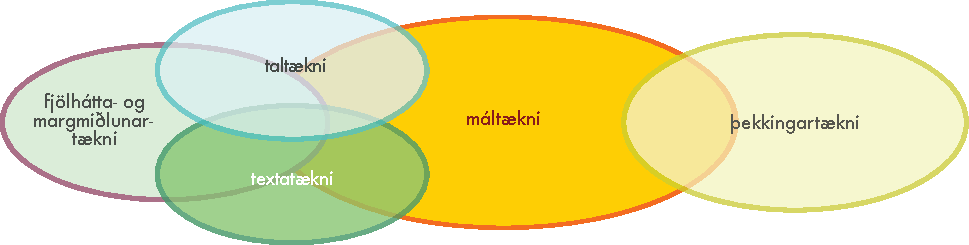
\includegraphics[width=\textwidth]{../_media/icelandic/language_technologies}
  \caption{Samhengi máltækninnar}
  \label{fig:ltincontext_is}
  \colorrule{grey3}{\textwidth}{1.5pt}
\end{figure*}

Í öllum samskiptum tengjum við tungumálið öðrum samskiptaháttum og upplýsingamiðlum -- tali getur fylgt látbragð og andlitstjáning. Stafrænir textar tengjast myndum og hljóði. Í kvikmyndum getur komið fram bæði talað og ritað mál. Tal- og textatækni skarast því og fléttast saman við margs konar aðra tækni sem greiðir fyrir úrvinnslu fjölhátta samskipta og margmiðlunargagna.

Hér á eftir verður fjallað um meginverksvið máltækni, þ.e. málrýni, vefleit, taltækni og vélþýðingar. Undir þetta fellur verkbúnaður og grundvallartækni eins og:

\begin{itemize}
\item stafrýni
\item ritstoð
\item tölvustutt tungumálanám
\item upplýsingaheimt 
\item útdráttur upplýsinga
\item samantekt texta
\item spurningasvörun
\item talkennsl
\item talgerving
\end{itemize}

Máltækni er mótað og öflugt rannsóknarsvið og hægt er að vísa á fjölda inngangstexta um sviðið, t.d. \cite{carstensen-etal1, jurafsky-martin01, manning-schuetze1, lt-world1, lt-survey1}.

Áður en ofannefndum notkunarsviðum og búnaði verða gerð skil verður högun dæmigerðs máltæknikerfis lýst stuttlega.

\subsection{Högun máltæknibúnaðar}

Í dæmigerðum hugbúnaði til málvinnslu felast nokkrar einingar sem endurspegla mismunandi þætti tungumálsins. Mynd~\ref{fig:textprocessingarch_is} sýnir mjög einfaldaða byggingu ritvinnslukerfis. Þrjár fyrstu einingarnar snúa að gerð og merkingu ílagstextans: 

\begin{figure*}[htb]
  \colorrule{grey3}{\textwidth}{1.5pt}
  \center
  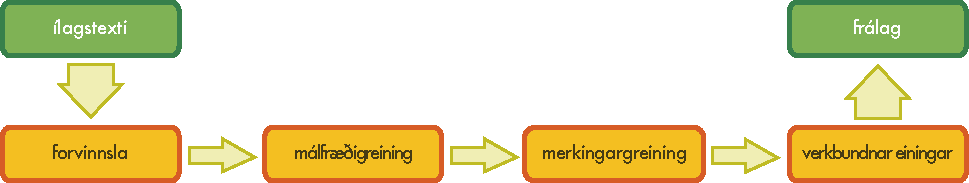
\includegraphics[width=\textwidth]{../_media/icelandic/text_processing_app_architecture}
  \caption{Dæmigerð kerfishögun við textavinnslu}
  \label{fig:textprocessingarch_is}
  \colorrule{grey3}{\textwidth}{1.5pt}
\end{figure*}

\begin{enumerate}
\item Forvinnsla: hreinsun gagna, afnám sniðs, greining ílagstungumáls, o.s.frv.
\item Málfræðigreining: sögnin fundin, andlög hennar og ákvæðisorð, og setningagerðin greind.
\item Merkingargreining: einræðing orða (fundið út hver er merking orðsins í tilteknu samhengi); greining endurvísunar (t.d. hvaða fornafn vísar til hvaða nafnorðs í setningunni) og staðgengla; og merking setningarinnar sýnd á þann hátt að tölva geti lesið hana.
\end{enumerate}

Eftir greiningu textans geta verkbundnar einingar séð um ýmsar aðrar aðgerðir, svo sem sjálfvirka samantekt ílagstexta og uppflettingu í gagnagrunni. Þetta er einfölduð lýsing á uppbyggingu verkbúnaðarins en gefur þó innsýn í það hversu flókinn máltæknibúnaður er. 

Að lokinni kynningu á helstu verksviðum máltækninnar verður gefið stutt yfirlit yfir yfirlit yfir núverandi stöðu máltæknirannsókna og máltæknimenntunar, og að lokum drepið á rannsóknarverkefni sem ýmist er lokið eða eru í gangi. Síðan verður gerð grein fyrir mati sérfræðinga á stöðu helstu máltæknitóla og málfanga út frá ýmsum mælikvörðum, s.s. aðgengi, þroska og gæðum. Heildarstaða máltækni fyrir íslensku er svo dregin saman í töflu (Mynd~\ref{fig:lrlttable_is}) í lok þessa kafla. Þau hugtök og málföng sem eru feitletruð í textanum er að finna í þessari töflu. Í framhaldi af þessu er máltæknistuðningur við íslensku borinn saman við stuðning við önnur tungumál sem fjallað er um í þessari ritröð.

\subsection{Helstu verksvið} 

Í þessum kafla verður fjallað um mikilvægustu máltæknitól og málföng, og gefið yfirlit yfir máltækni á Íslandi.chweiz. 

\subsubsection{Málrýni}

Flestir sem hafa unnið með ritvinnslukerfi eins og Microsoft Word vita að í því er stafrýnir sem bendir á stafsetningarvillur og stingur upp á leiðréttingum. Fyrstu stafrýnarnir báru orðin í textanum saman við safn rétt ritaðra orða. Nú er þessi hugbúnaður mun þróaðri. Með því að nota sérhæfð algrím til \textbf{textagreiningar} má greina villur í beygingu (svo sem ranga eignarfallsendingu) og setningagerð, eins og þegar sögnina vantar eða þegar ósamræmi er á milli sagnar og frumlags (t.d. \textit{ég *skrifar bréf}). Hins vegar munu fæstir stafrýnar finna villur í eftirfarandi dæmum:

\begin{itemize}
\item Ég var um þetta leiti á næsta leyti.
\item Hún segir að móðir sýn hafi aðra sín á málið.
\item Hann þótti hafa stirt stöðu sína.
\end{itemize}

Til þess að hægt sé að fást við slíkar villur þarf að greina samhengi textans, t.d. þegar ákveða skal hvort íslenskt lýsingarorð eigi að vera með einu \textit{n}-i (kvenkyn) eða tveim (karlkyn), eins og í eftirfarandi dæmi:

\begin{itemize}
\item Hann er farinn.
\item Hún er farin.
\end{itemize}

Greining slíkra villna byggist ýmist á sérstakri málfræðilýsingu fyrir hvert tungumál, sem mikinn tíma og sérþekkingu þarf til að fella inn í hugbúnaðinn, eða á tölfræðilegu mállíkani. Slíkt líkan reiknar líkurnar á því að tiltekið orð birtist í ákveðnu umhverfi (t.d. eftir því hvaða orð fara á undan og á eftir). Til dæmis er \textit{hann er farinn} líkleg orðaruna en \textit{hún er farinn} er það ekki. Tölfræðilegu mállíkani af þessu tagi má koma upp á sjálfvirkan hátt með því að nota mikið af (réttum) málgögnum (\textbf{málheild}). Báðar aðferðirnar (reglusmíði og tölfræðilíkan) hafa einkum verið þróaðar fyrir ensk málföng og það er ekki auðvelt að yfirfæra þær á íslensku sem hefur sveigjanlegri orðaröð, ótakmarkaða möguleika á samsetningu orða og ríkulegra beygingarkerfi. \boxtext{Málrýni er ekki bundin við ritvinnslukerfi; hún er líka notuð í ritstoðarkerfum.} Málrýni er ekki bundin við ritvinnslukerfi; hún er líka notuð í ritstoðarkerfum, þ.e. hugbúnaðarumhverfi til að skrifa handbækur og önnur rit samkvæmt ákveðnum stöðlum fyrir flókna upplýsingatækni, heilbrigðisgeirann, verkfræði og fleira. Af ótta við kvartanir og skaðabótakröfur viðskiptavina vegna rangrar notkunar sem rekja má til illskiljanlegra leiðbeininga leggja fyrirtæki sífellt meiri áherslu á gæði tæknilegra leiðbeininga, á sama tíma og þau stefna á alþjóðlegan markað (með þýðingum og staðfærslu). Framfarir í málvinnslu hafa leitt til þróunar á ritstoðarbúnaði sem aðstoðar höfunda tæknilegra leiðbeininga við að velja orð og setningagerð sem samræmist iðnaðarreglum og skorðum fyrirtækja á notkun íðorða.

\begin{figure*}[htb]
  \colorrule{grey3}{\textwidth}{1.5pt}
  \center
  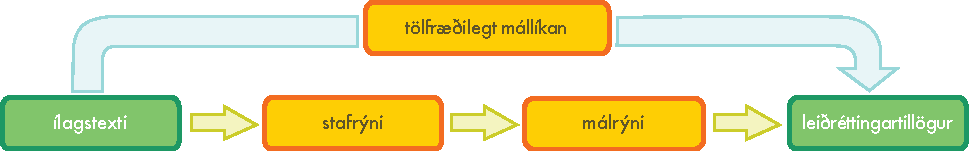
\includegraphics[width=\textwidth]{../_media/icelandic/language_checking}
  \caption{Málrýni (tölfræðileg; reglubyggð)}
  \label{fig:langcheckingaarch_is}
  \colorrule{grey3}{\textwidth}{1.5pt}
\end{figure*}

Stafrýnir hefur verið til fyrir íslensku frá því seint á níunda áratugnum þegar Friðrik Skúlason ehf. (Frisk Software) þróaði stafsetningaforritið \textit{Púka}. Forritið hefur síðan verið uppfært og endurbætt. Það er til fyrir MS Office og er mikið notað. Aðrir stafrýnar hafa einnig verið hannaðir. Árið 2002 þróaði hollenska fyrirtækið Polderland stafrýni fyrir MS Office og einnig er til stafrýnir í opnum hugbúnaði fyrir GNU/Linux forrit, byggður á Aspell. Þessi forrit skoða eingöngu stök orð og ráða því ekki við margar algengar stafsetningarvillur. Frumgerð að samhengisháðum stafrýni hefur verið felld inn í LanguageTool\cite{lto1} og vinnur með OpenOffice. Sá stafrýnir gæti hugsanlega myndað grunninn að málfræðirýni, en slíkt forrit er ekki til fyrir íslensku. 

Fyrir utan stafrýna og ritstoð er málrýning einnig mikilvæg fyrir tölvustutt tungumálanám og henni er líka beitt við sjálfvirka leiðréttingu á fyrirspurnum sem sendar eru vefleitarvélum eins og tillögukerfi Google \textit{Áttirðu við}:

\subsubsection{Vefleit}

Leit á vefnum, svo og á innri netum og í stafrænum bókasöfnum, er væntanlega það svið þar sem máltækni er mest notuð nú á dögum, en er þó fremur skammt á veg komin. Leitarvélin Google, sem kom fram á sjónarsviðið 1998, er nú notuð í 80\% allra vefleita í heiminum \cite{spi1}.  Síðan 2004 hefur sögnin  \textit{gúg(g)la} verið notuð í íslensku þótt hún hafi ekki enn komist í prentaðar orðabækur. Hvorki leitarviðmót Google né framsetning niðurstaðna hefur tekið grundvallarbreytingum frá fyrstu útgáfu. Í nýjustu útgáfu býður Google reyndar upp á leiðréttingar á ranglega stafsettum orðum og hefur nú bætt við merkingarlegum leitarmöguleikum sem geta bætt nákvæmni leitarinnar með því að greina merkingu orða í samhengi leitarorðsins\cite{pc1}.  Velgengni Google sýnir að með stóru gagnasafni og skilvirkum aðferðum við að lykla gögnin getur tölfræðileg aðferð skilað vel viðunandi niðurstöðum.

\begin{figure*}[htb]
  \colorrule{grey3}{\textwidth}{1.5pt}
  \center
  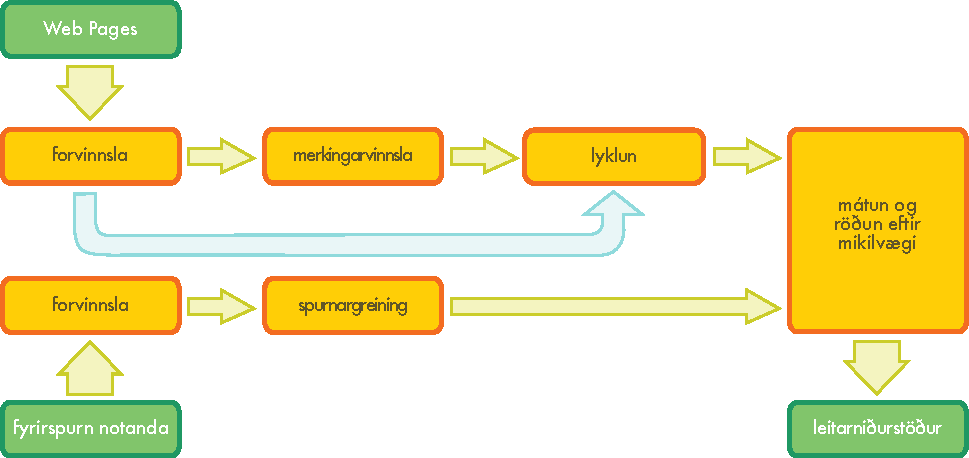
\includegraphics[width=\textwidth]{../_media/icelandic/web_search_architecture}
  \caption{Vefleit}
  \label{fig:websearcharch_is}
  \colorrule{grey3}{\textwidth}{1.5pt}
\end{figure*}

Þegar um flóknari upplýsingaleit er að ræða er nauðsynlegt að nýta dýpri málfræðiþekkingu til \textbf{textatúlkunar}. Tilraunir með \textbf{orðaföng} eins og tölvutæk samheitasöfn og verufræðileg málföng (s.s. WordNet fyrir ensku og GermaNet fyrir þýsku) hafa sýnt verulega bættan árangur í að finna síður þar sem samheiti við leitarorðið koma fyrir, svo sem  \textit{hagnaður}, \textit{arður}, \textit{gróði} og  \textit{ábati} eða jafnvel fjarskyldari orð.

Næsta kynslóð leitarvéla verður að vera útbúin mun þróaðri máltækni, einkum til að ráða við leitartexta í formi spurningar eða annars konar setningar í stað einstakra leitarorða. Til að bregðast við fyrirspurninni „Láttu mig fá lista yfir öll fyrirtæki sem voru yfirtekin af öðrum fyrirtækjum síðustu fimm árin“ þarf máltæknikerfið að greina setningagerð og merkingu fyrirspurnarinnar og hafa atriðisorðaskrá til að kalla fram viðeigandi skjöl á fljótvirkan hátt. Til að unnt sé að gefa viðunandi svar þarf að beita setningalegri þáttun til greiningar á málfræðilegri formgerð setningarinnar og greina að verið sé að leita að fyrirtækjum sem hafa verið yfirtekin en ekki þeim fyrirtækjum sem tóku yfir önnur fyrirtæki. Þá þarf að skilgreina sambandið  \textit{síðustu fimm} ár svo hægt sé að ákvarða við hvaða ár er átt. Að lokum þarf að máta leitarfyrirspurnina við ógrynni af óskipulögðum gögnum svo að finna megi upplýsingarnar sem leitað er að. Þetta er kallað ‘upplýsingaheimt’ og felur í sér leit að skjölum og vægisröðun þeirra. Til þess að hægt sé að búa til lista yfir fyrirtæki þarf kerfið einnig að þekkja ákveðinn orðastreng í skjali sem nafn fyrirtækis, en það ferli kallast ‘nafnakennsl’. \boxtext{Næsta kynslóð leitarvéla verður að vera útbúin mun þróaðri máltækni.} Enn meiri ögrun felst í því að máta leitarfyrirspurnina við skjöl á öðrum tungumálum. Þvermála upplýsingaheimt felur í sér sjálfvirka þýðingu leitarfyrirspurnar yfir á öll möguleg tungumál og síðan þýðingu niðurstaðnanna aftur yfir á markmálið.

Nú er gögn í auknum mæli að finna á öðru sniði en sem texta og því er orðin til þörf á þjónustu sem gefur kost á margmiðlunarupplýsingaheimt með því að leita að myndum, hljóði eða myndböndum. Þegar um er að ræða hljóð- og myndbandsskrár þarf sérstök talkennslaeining að breyta tali í texta (eða hljóðritun) sem síðan er hægt að máta við leitarfyrirspurnina.

Í beygingarmálum eins og íslensku er mikilvægt að hægt sé að leita að öllum beygingarmyndum orðs í einu í stað þess að þurfa að leita að hverri mynd sérstaklega. Þetta má gera með aðstoð gagnagrunnsins \textit{Beygingarlýsing íslensks nútímamáls}, \textit{BÍN}\cite{bin1}, sem þróaður hefur verið á Stofnun Árna Magnússonar í íslenskum fræðum. Gagnagrunnurinn hefur að geyma um það bil 280.000 beygingardæmi með meira en 5,8 milljónum beygingarmynda. Hver færsla inniheldur nefnimyndina, orðmyndina, orðflokkinn og beygingarþætti nafnorða, sérnafna, lýsingarorða, sagna og atviksorða.

Fyrir nokkrum árum þróaði fyrirtækið Spurl leitarvélina \textit{Emblu} sem nýtti þennan gagnagrunn. Sama algrím er notað við leit í íslensku símaskránni og á nokkrum öðrum síðum. Google leitarvélin er nú búin svipuðum hæfileikum, en þó ekki eins margþættum. Engin sérhæfð leitarvél fyrir íslensku er til eins og er, fyrir utan íslenska viðmótið í Google, og ekki er verið að vinna að slíkri leitarvél.
  
\subsubsection{Talsamskipti}

Talsamskipti eru eitt margra verksviða sem byggjast á taltækni, þ.e. tækni til að vinna með talað mál. Talsamskiptatækni er notuð til að smíða viðmót sem gerir notandanum kleift að tala við tölvuna í stað þess að nota tölvuskjáinn, lyklaborð og mús. Nú á dögum nýta fyrirtæki raddstýrð notendaviðmót í ýmiss konar sjálfvirkri og hálfsjálfvirkri símaþjónustu við viðskiptavini, starfsmenn eða viðskiptafélaga. Helstu atvinnugreinar sem nýta slík raddstýrð viðmót eru bankastarfsemi, birgjar, almenningssamgöngur og fjarskiptafyrirtæki. Talsamskiptatækni má t.d. einnig nota í viðmóti leiðsögutækja í bílum og í stað myndræns viðmóts og snertiskjáa sem notendaviðmót í snjallsímum. \boxtext{Taltækni er notuð til að smíða viðmót sem gerir notandanum kleift að tala við tölvuna í stað þess að nota tölvuskjáinn, lyklaborð og mús.}

\begin{figure*}[htb]
  \colorrule{grey3}{\textwidth}{1.5pt}
  \center 
  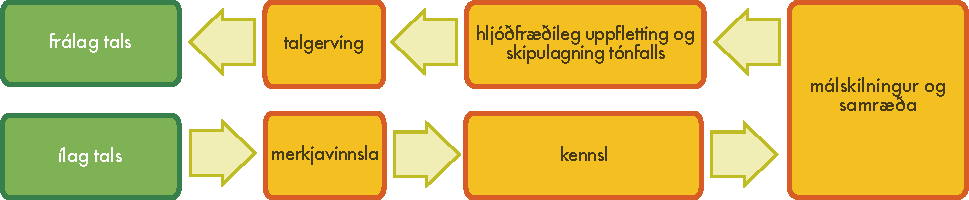
\includegraphics[width=\textwidth]{../_media/icelandic/simple_speech-based_dialogue_architecture}
  \caption{Talsamskiptakerfi}
  \label{fig:dialoguearch_is}
  \colorrule{grey3}{\textwidth}{1.5pt}
\end{figure*}

Talsamskipti byggjast á ferns konar grundvallartækni:

\begin{enumerate}
\item Sjálfvirk \textbf{talkennsl} ákvarða hvaða orð notandinn segir í tiltekinni segð. 
\item Málskilningur greinir setningafræðilega formgerð segðarinnar og túlkar hana út frá viðkomandi kerfi.
\item Samræðustjóri ákvarðar hvað þarf að gera út frá ílagi notandans og möguleikum kerfisins.
\item \textbf{Talgerving} breytir svari kerfisins í hljóð sem notandinn nemur. 
\end{enumerate}

Eitt erfiðasta viðfangsefni talkennslabúnaðar er að greina rétt þau orð sem notandinn segir. Því þarf annaðhvort að takmarka hugsanlegar segðir notandans við afmarkað mengi lykilorða eða byggja upp mállíkön sem ná yfir stóran hluta segða í eðlilegu máli. Með vélrænum námsaðferðum er líka hægt að koma upp mállíkönum á sjálfvirkan hátt úr \textbf{talmálsheildum}, stórum söfnum hljóðskráa með textaumritun. Takmörkun leyfilegra segða leiðir venjulega til þvingaðrar notkunar á talviðmótinu og getur haft þau áhrif að notendur taki því ekki vel; en smíði viðamikils mállíkans, fínstilling þess og viðhald eykur kostnaðinn við kerfið verulega. Raddstýrð notendaviðmót sem nýta mállíkan og gefa notandanum sveigjanleika í því hvernig hann ber fram erindi sitt í byrjun -- t.d. heilsa með \textit{Hvað get ég gert fyrir þig}? -- eru yfirleitt sjálfvirk og fá jákvæðari viðbrögð notenda.

Fyrirtæki nota yfirleitt upptökur með lestri atvinnumanna til að mynda frálag talviðmótsins. Í stöðluðum segðum þar sem orðalagið er ekki háð tilteknu samhengi eða ákveðnum notanda getur þetta verið fullkomlega nóg til að notandinn sé sáttur. En þegar segðirnar eru breytilegar getur tónfallið orðið óeðlilegt vegna þess að bútar úr mismunandi hljóðskrám eru tengdir saman. Talgervlar eru sífellt að verða betri í því að skila breytilegum segðum sem hljóma eðlilega, en þó má enn bæta þá.

Viðmót á talsamskiptamarkaðnum hafa verið stöðluð umtalsvert á undanförnum áratug að því er snýr að hinum ýmsu tæknieiningum þeirra. Einnig hefur orðið veruleg markaðssamþjöppun fyrirtækja í talkennslum og talgervingu. Á innanlandsmarkaði í G20-löndunum (fjölmennum og efnahagslega sterkum löndum) hafa fimm alþjóðleg fyrirtæki verið ríkjandi, og í Evrópu einkum tvö -- Nuance (bandarískt) og Loquendo (ítalskt). Árið 2011 tilkynnti Nuance um yfirtöku Loquendo þannig að markaðssamþjöppunin heldur enn áfram.

Tveir talgervlar fyrir íslensku hafa verið settir á markað. Formendabyggður talgervill var upphaflega gerður í kringum 1990. Hann var einkum notaður af blindum og sjónskertum en þótti ekki nógu fullkominn til notkunar í kerfum og verkbúnaði fyrir almennan markað. 

Árið 2005 var búinn til nýr talgervill í samvinnu Háskóla Íslands, Símans og Hex hugbúnaðar. Talgervillinn byggðist á tækni Nuance sem sá um þjálfun hans. Hann hefur verið notaður dálítið í verkbúnaði fyrir almennan markað en mörgum notendum finnst raddgæðin ekki fullnægjandi. Þar sem gæði tiltækra talgervla þykja ekki nógu mikil hefur aðalnotandi þeirra, Blindrafélagið, ákveðið að þróa nýjan talgervil í samvinnu við Háskóla Íslands, Háskólann í Reykjavík og pólska hugbúnaðarfyrirtækið Ivona. Gangi allt samkvæmt áætlun verður talgervillinn tilbúinn árið 2012\cite{tal1}.

Stakorðagreinir var þróaður fyrir íslensku árið 2003. Hann skilaði góðum árangri í greiningu, eða um 97\% nákvæmni. Þá hefur íslenskur stúdent við Tokyo Institute of Technology hannað frumgerð af kerfi fyrir sjálfvirk orðaflaumskennsl í íslensku. Kerfið náði 67,5\% orðanákvæmni\cite{hind1}. Hvorugt þessara kerfa hefur verið notað í verkbúnað fyrir almennan markað. Um mitt ár 2011 hófu Háskólinn í Reykjavík og Máltæknisetur samvinnu við Google um undirbúning að smíði talþekkjara fyrir íslensku\cite{alm1}.

Miklar breytingar má sjá framundan vegna útbreiðslu snjallsíma sem nýs vettvangs fyrir tengsl fyrirtækja og viðskiptavina, í viðbót við venjulega síma, vefinn og tölvupóst. Þessar breytingar munu einnig hafa áhrif á nýtingu taltækninnar. Notkun á raddstýrðu viðmóti venjulegra síma mun fara minnkandi en mikilvægi talaðs máls sem notendavæns samskiptamáta við snjallsíma er sífellt að aukast. Það sem knýr þessa þróun er einkum aukin nákvæmni í talkennslum óháðum mælanda í þeim upplestrarkerfum sem þegar eru í boði sem miðlæg þjónusta fyrir notendur snjallsíma.

\subsubsection{Vélþýðingar}

Hugmyndina að því að nota tölvur til að þýða mannleg mál má rekja til ársins 1946 og var henni fylgt eftir með umtalsverðu fjármagni til rannsókna á sjötta áratug síðustu aldar og aftur á þeim níunda. Samt sem áður hafa \textbf{vélþýðingar} ekki náð að standa undir þeim væntingum um sjálfvirkar þýðingar milli tungumála sem þær gáfu á upphafsárunum.\boxtext{Einfaldasta gerð vélrænna þýðinga felst í því að skipta út orðum í öðru málinu fyrir orð úr hinu málinu.}Einfaldasta gerð vélþýðinga felst í því að skipta út orðum í öðru málinu fyrir orð úr hinu málinu. Þetta getur verið gagnlegt á efnissviðum þar sem notað er mjög afmarkað og staðlað mál, svo sem í veðurfregnum. En til þess að þýðing á máli sem er ekki eins staðlað verði viðunandi þarf að fella stærri textaeiningar (orðasambönd, málsgreinar, jafnvel heilar efnisgreinar) sem nákvæmast að samsvarandi einingum í markmálinu. Helstu vandkvæðin felast í því að mannlegt mál er margrætt. Margræðni skapar vanda á mörgum sviðum, svo sem við einræðingu merkingar á orðasviðinu (\textit{villa} er bæði ‘mistök’ og ‘veglegt hús’), og fallstjórn á setningafræðisviðinu, eins og í:

\begin{itemize}
\item Konan sá bílinn og \textbf{maðurinn hennar} líka.
\item Konan sá bílinn og \textbf{manninn sinn} líka.
\item {[}The woman saw the car and her husband, too.{]}
\end{itemize}

Ein leið til að búa til vélþýðingarkerfi er að nota málfræðilegar reglur. Þegar þýtt er á milli náskyldra tungumála getur aðferð beinna umskipta verið fýsileg, eins og í dæminu hér að ofan. En reglubyggð kerfi (byggð á málfræðilegri þekkingu) greina oft ílagstextann og skapa táknbyggt millistig sem texti markmálsins er síðan leiddur af. Árangur þessarar aðferðar er undir því kominn að til sé yfirgripsmikið orðasafn með beygingarlegum, setningafræðilegum og merkingarlegum upplýsingum, ásamt stóru safni málfræðireglna sem þjálfaðir málfræðingar hafa smíðað af vandvirkni. Það er langt og þar með dýrt ferli að koma þessum forsendum upp.

\begin{figure*}[htb]
  \colorrule{grey3}{\textwidth}{1.5pt}
  \center
  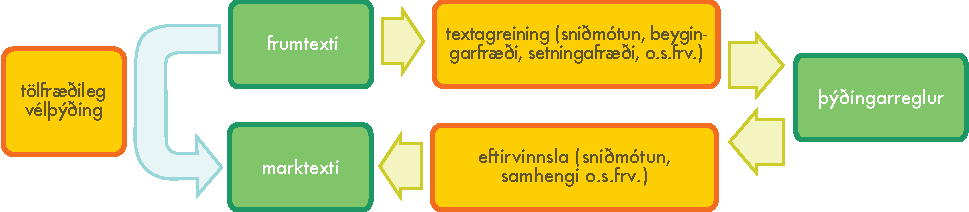
\includegraphics[width=\textwidth]{../_media/icelandic/machine_translation}
  \caption{Vélþýðingar (tölfræðilegar; reglubyggðar)}
  \label{fig:mtarch_is}
  \colorrule{grey3}{\textwidth}{1.5pt}
\end{figure*}

Á síðari hluta níunda áratugarins þegar tölvur urðu öflugri og ódýrari jókst áhugi á að nýta tölfræðileg líkön í vélþýðingum. Tölfræðileg líkön byggjast á greiningu tvímála málheilda, svo sem Europarl \textbf{hliðstæðu málheildarinnar}, sem hefur að geyma þingskjöl Evrópuþingsins á 11 Evrópumálum. Ef nóg er af gögnum virka tölfræðilegar vélþýðingar nægilega vel til þess að gefa nokkurn veginn rétta merkingu texta á erlendu tungumáli með því að skoða samhliða texta og greina líkleg orðamynstur. Ólíkt þekkingarknúnum kerfum skila tölfræðilegar (eða gagnaknúnar) vélþýðingar oft málfræðilega röngu frálagi. Kosturinn við gagnaknúnar vélþýðingar er sá að þær eru ekki eins mannaflsfrekar, og einnig geta þær ráðið við ýmis málleg sérkenni (s.s. málshætti og orðtök) sem fara forgörðum í þekkingarknúnu kerfunum.

Styrkleikar og veikleikar þekkingarknúinna og gagnaknúinna vélþýðinga eru á mismunandi sviðum og því einbeita vísindamenn sér núorðið að blönduðum aðferðum sem sameina aðferðafræði beggja. Ein aðferðin er sú að nota bæði þekkingarknúið og gagnaknúið kerfi og láta svo sérstaka valeiningu ákveða hvert sé besta frálag hverrar setningar. Þegar um er að ræða lengri setningar en 12 orð verða niðurstöðurnar þó sjaldnast fullkomnar. Betri aðferð er að sameina bestu hluta hverrar setningar úr mörgum frálögum; þetta getur verið tiltölulega flókið þar sem samsvaranir mismunandi möguleika eru ekki alltaf augljósar og því þarf að samskipa þeim.\boxtext{Vélþýðingar milli íslensku og annarra mála eru mjög snúnar.} Vélþýðingar milli íslensku og annarra mála eru mjög snúnar. Vegna fjölbreyttra möguleika til smíði samsettra orða er oft erfitt að greina orð og hafa nægilega yfirgripsmikið orðasafn; frjáls orðaröð og sagnaragnir skapa ýmis vandamál í greiningu, og auðugt beygingarkerfi veldur vandkvæðum við að merkja rétt öll beygingaratriði s.s. kyn, fall, tölu, hátt, tíð, o.s.frv.

Þróun vélþýðinga fyrir íslensku hefur ekki orðið ýkja mikil. Stefán Briem, sjálfstætt starfandi fræðimaður, hefur unnið að vélþýðingum síðan snemma á níunda áratugnum og hefur hannað vélþýðingarkerfi fyrir íslensku. Árið 2008 opnaði hann á vefnum ókeypis þjónustu sem býður upp á þýðingar milli íslensku og þriggja annarra tungumála (ensku, dönsku og esperantó)\cite{tut1}. Hrafn Loftsson, kennari við Háskólann í Reykjavík, og samstarfsmenn hans hafa hannað reglubyggt grófþýðingakerfi úr íslensku á ensku, grundvallað á Apertium-verkvangnum\cite{ape1}. Forútgáfa er nú á vefnum\cite{ape2}. Google Translate hefur gefið kost á þýðingum úr og á íslensku síðan 2009. Gæðin voru heldur lítil í byrjun en hafa aukist.

Enn má auka gæði vélþýðingarkerfa verulega. Helstu vandkvæðin felast í aðlögun málfanganna að tilteknum efnissviðum eða notendahópum, og samþættingu tækninnar við vinnuferli sem nú þegar eru búin íðorðagrunni og þýðingarminni. Annað vandamál er að flest núverandi kerfi eru miðuð við ensku og sinna einungis þýðingum milli íslensku og örfárra annarra mála. Þetta leiðir til árekstra í þýðingarflæðinu og þvingar notendur vélrænna þýðinga til að læra á mismunandi orðakótunartól fyrir mismunandi kerfi.

Matskeppnir nýtast vel til að bera saman gæði vélþýðingarkerfa, mismunandi aðferðafræði og frammistöðu þeirra gagnvart mismunandi tungumálapörum. Taflan hér á eftir, sem unnin var innan Euromatrix+ verkefnis Evrópusambandsins, sýnir útkomu allra para milli 22 af 23 opinberum tungumálum Evrópusambandsins. (Írska var ekki með í samanburðinum.) Niðurstöðum er raðað samkvæmt BLEU einkunnakvarða, þar sem hærri einkunn fæst fyrir betri þýðingu\cite{bleu1}.  (Mennskur þýðandi myndi ná um 80 stigum.)

Bestu niðurstöðurnar (í grænum og bláum lit) fengust fyrir tungumál sem njóta góðs af umfangsmiklum samhæfðum rannsóknaráætlunum, sem og af tilvist margra samhliða málheilda (t.d. enska, franska, hollenska, spænska og þýska). Þau tungumál sem verr koma út eru merkt með rauðu. Þau skortir annaðhvort slíkar rannsóknaráætlanir eða eru eðlisólík öðrum tungumálum (t.d. ungverska, maltneska og finnska).

\begin{figure*}[htbp]
  \centering
  \setlength{\tabcolsep}{0.17em}
  \small
  \begin{tabular}{>{\columncolor{corange1}}cccccccccccccccccccccccc}
    & \multicolumn{22}{>{\columncolor{corange1}}c}{Markmál -- \textcolor{grey1}{Target language}}\\\addlinespace[{-.009cm}]
    \rowcolor{corange1}  & EN & BG & DE & CS & DA & EL & ES & ET & FI & FR & HU & IT & LT & LV & MT & NL & PL & PT & RO & SK & SL & SV\\
    EN & -- & \textcolor{blue}{40.5} & \textcolor{blue}{46.8} & \textcolor{green2}{52.6} & \textcolor{green2}{50.0} & \textcolor{blue}{41.0} & \textcolor{green2}{55.2} & \textcolor{purple}{34.8} & \textcolor{purple}{38.6} & \textcolor{green2}{50.1} & \textcolor{purple}{37.2} & \textcolor{green2}{50.4} & \textcolor{purple}{39.6} & \textcolor{blue}{43.4} & \textcolor{purple}{39.8} & \textcolor{green2}{52.3} & \textcolor{blue}{49.2} & \textcolor{green2}{55.0} & \textcolor{blue}{49.0} & \textcolor{blue}{44.7} & \textcolor{green2}{50.7} & \textcolor{green2}{52.0}\\
    BG & \textcolor{green}{61.3} & -- & \textcolor{purple}{38.7} & \textcolor{purple}{39.4} & \textcolor{purple}{39.6} & \textcolor{purple}{34.5} & \textcolor{blue}{46.9} & \textcolor{red3}{25.5} & \textcolor{red3}{26.7} & \textcolor{blue}{42.4} & \textcolor{red3}{22.0} & \textcolor{blue}{43.5} & \textcolor{red3}{29.3} & \textcolor{red3}{29.1} & \textcolor{red3}{25.9} & \textcolor{blue}{44.9} & \textcolor{purple}{35.1} & \textcolor{blue}{45.9} & \textcolor{purple}{36.8} & \textcolor{purple}{34.1} & \textcolor{purple}{34.1} & \textcolor{purple}{39.9}\\
    DE & \textcolor{green2}{53.6} & \textcolor{red3}{26.3} & -- & \textcolor{purple}{35.4} & \textcolor{blue}{43.1} & \textcolor{purple}{32.8} & \textcolor{blue}{47.1} & \textcolor{red3}{26.7} & \textcolor{red3}{29.5} & \textcolor{purple}{39.4} & \textcolor{red3}{27.6} & \textcolor{blue}{42.7} & \textcolor{red3}{27.6} & \textcolor{purple}{30.3} & \textcolor{red2}{19.8} & \textcolor{green2}{50.2} & \textcolor{purple}{30.2} & \textcolor{blue}{44.1} & \textcolor{purple}{30.7} & \textcolor{red3}{29.4} & \textcolor{purple}{31.4} & \textcolor{blue}{41.2}\\
    CS & \textcolor{green2}{58.4} & \textcolor{purple}{32.0} & \textcolor{blue}{42.6} & -- & \textcolor{blue}{43.6} & \textcolor{purple}{34.6} & \textcolor{blue}{48.9} & \textcolor{purple}{30.7} & \textcolor{purple}{30.5} & \textcolor{blue}{41.6} & \textcolor{red3}{27.4} & \textcolor{blue}{44.3} & \textcolor{purple}{34.5} & \textcolor{purple}{35.8} & \textcolor{red3}{26.3} & \textcolor{blue}{46.5} & \textcolor{purple}{39.2} & \textcolor{blue}{45.7} & \textcolor{purple}{36.5} & \textcolor{blue}{43.6} & \textcolor{blue}{41.3} & \textcolor{blue}{42.9}\\
    DA & \textcolor{green2}{57.6} & \textcolor{red3}{28.7} & \textcolor{blue}{44.1} & \textcolor{purple}{35.7} & -- & \textcolor{purple}{34.3} & \textcolor{blue}{47.5} & \textcolor{red3}{27.8} & \textcolor{purple}{31.6} & \textcolor{blue}{41.3} & \textcolor{red3}{24.2} & \textcolor{blue}{43.8} & \textcolor{red3}{29.7} & \textcolor{purple}{32.9} & \textcolor{red3}{21.1} & \textcolor{blue}{48.5} & \textcolor{purple}{34.3} & \textcolor{blue}{45.4} & \textcolor{purple}{33.9} & \textcolor{purple}{33.0} & \textcolor{purple}{36.2} & \textcolor{blue}{47.2}\\
    EL & \textcolor{green2}{59.5} & \textcolor{purple}{32.4} & \textcolor{blue}{43.1} & \textcolor{purple}{37.7} & \textcolor{blue}{44.5} & -- & \textcolor{green2}{54.0} & \textcolor{red3}{26.5} & \textcolor{red3}{29.0} & \textcolor{blue}{48.3} & \textcolor{red3}{23.7} & \textcolor{blue}{49.6} & \textcolor{red3}{29.0} & \textcolor{purple}{32.6} & \textcolor{red3}{23.8} & \textcolor{blue}{48.9} & \textcolor{purple}{34.2} & \textcolor{green2}{52.5} & \textcolor{purple}{37.2} & \textcolor{purple}{33.1} & \textcolor{purple}{36.3} & \textcolor{blue}{43.3}\\
    ES & \textcolor{green}{60.0} & \textcolor{purple}{31.1} & \textcolor{blue}{42.7} & \textcolor{purple}{37.5} & \textcolor{blue}{44.4} & \textcolor{purple}{39.4} & -- & \textcolor{red3}{25.4} & \textcolor{red3}{28.5} & \textcolor{green2}{51.3} & \textcolor{red3}{24.0} & \textcolor{green2}{51.7} & \textcolor{red3}{26.8} & \textcolor{purple}{30.5} & \textcolor{red3}{24.6} & \textcolor{blue}{48.8} & \textcolor{purple}{33.9} & \textcolor{green2}{57.3} & \textcolor{purple}{38.1} & \textcolor{purple}{31.7} & \textcolor{purple}{33.9} & \textcolor{blue}{43.7}\\
    ET & \textcolor{green2}{52.0} & \textcolor{red3}{24.6} & \textcolor{purple}{37.3} & \textcolor{purple}{35.2} & \textcolor{purple}{37.8} & \textcolor{red3}{28.2} & \textcolor{blue}{40.4} & -- & \textcolor{purple}{37.7} & \textcolor{purple}{33.4} & \textcolor{purple}{30.9} & \textcolor{purple}{37.0} & \textcolor{purple}{35.0} & \textcolor{purple}{36.9} & \textcolor{red3}{20.5} & \textcolor{blue}{41.3} & \textcolor{purple}{32.0} & \textcolor{purple}{37.8} & \textcolor{red3}{28.0} & \textcolor{purple}{30.6} & \textcolor{purple}{32.9} & \textcolor{purple}{37.3}\\
    FI & \textcolor{blue}{49.3} & \textcolor{red3}{23.2} & \textcolor{purple}{36.0} & \textcolor{purple}{32.0} & \textcolor{purple}{37.9} & \textcolor{red3}{27.2} & \textcolor{purple}{39.7} & \textcolor{purple}{34.9} & -- & \textcolor{red3}{29.5} & \textcolor{red3}{27.2} & \textcolor{purple}{36.6} & \textcolor{purple}{30.5} & \textcolor{purple}{32.5} & \textcolor{red2}{19.4} & \textcolor{blue}{40.6} & \textcolor{red3}{28.8} & \textcolor{purple}{37.5} & \textcolor{red3}{26.5} & \textcolor{red3}{27.3} & \textcolor{red3}{28.2} & \textcolor{purple}{37.6}\\
    FR & \textcolor{green}{64.0} & \textcolor{purple}{34.5} & \textcolor{blue}{45.1} & \textcolor{purple}{39.5} & \textcolor{blue}{47.4} & \textcolor{blue}{42.8} & \textcolor{green}{60.9} & \textcolor{red3}{26.7} & \textcolor{purple}{30.0} & -- & \textcolor{red3}{25.5} & \textcolor{green2}{56.1} & \textcolor{red3}{28.3} & \textcolor{purple}{31.9} & \textcolor{red3}{25.3} & \textcolor{green2}{51.6} & \textcolor{purple}{35.7} & \textcolor{green}{61.0} & \textcolor{blue}{43.8} & \textcolor{purple}{33.1} & \textcolor{purple}{35.6} & \textcolor{blue}{45.8}\\
    HU & \textcolor{blue}{48.0} & \textcolor{red3}{24.7} & \textcolor{purple}{34.3} & \textcolor{purple}{30.0} & \textcolor{purple}{33.0} & \textcolor{red3}{25.5} & \textcolor{purple}{34.1} & \textcolor{red3}{29.6} & \textcolor{red3}{29.4} & \textcolor{purple}{30.7} & -- & \textcolor{purple}{33.5} & \textcolor{red3}{29.6} & \textcolor{purple}{31.9} & \textcolor{red2}{18.1} & \textcolor{purple}{36.1} & \textcolor{red3}{29.8} & \textcolor{purple}{34.2} & \textcolor{red3}{25.7} & \textcolor{red3}{25.6} & \textcolor{red3}{28.2} & \textcolor{purple}{30.5}\\
    IT & \textcolor{green}{61.0} & \textcolor{purple}{32.1} & \textcolor{blue}{44.3} & \textcolor{purple}{38.9} & \textcolor{blue}{45.8} & \textcolor{blue}{40.6} & \textcolor{red3}{26.9} & \textcolor{red3}{25.0} & \textcolor{red3}{29.7} & \textcolor{green2}{52.7} & \textcolor{red3}{24.2} & -- & \textcolor{red3}{29.4} & \textcolor{purple}{32.6} & \textcolor{red3}{24.6} & \textcolor{green2}{50.5} & \textcolor{purple}{35.2} & \textcolor{green2}{56.5} & \textcolor{purple}{39.3} & \textcolor{purple}{32.5} & \textcolor{purple}{34.7} & \textcolor{blue}{44.3}\\
    LT & \textcolor{green2}{51.8} & \textcolor{red3}{27.6} & \textcolor{purple}{33.9} & \textcolor{purple}{37.0} & \textcolor{purple}{36.8} & \textcolor{red3}{26.5} & \textcolor{red3}{21.1} & \textcolor{purple}{34.2} & \textcolor{purple}{32.0} & \textcolor{purple}{34.4} & \textcolor{red3}{28.5} & \textcolor{purple}{36.8} & -- & \textcolor{blue}{40.1} & \textcolor{red3}{22.2} & \textcolor{purple}{38.1} & \textcolor{purple}{31.6} & \textcolor{purple}{31.6} & \textcolor{red3}{29.3} & \textcolor{purple}{31.8} & \textcolor{purple}{35.3} & \textcolor{purple}{35.3}\\
    LV & \textcolor{green2}{54.0} & \textcolor{red3}{29.1} & \textcolor{purple}{35.0} & \textcolor{purple}{37.8} & \textcolor{purple}{38.5} & \textcolor{red3}{29.7} & \textcolor{red2}{8.0} & \textcolor{purple}{34.2} & \textcolor{purple}{32.4} & \textcolor{purple}{35.6} & \textcolor{red3}{29.3} & \textcolor{purple}{38.9} & \textcolor{purple}{38.4} & -- & \textcolor{red3}{23.3} & \textcolor{blue}{41.5} & \textcolor{purple}{34.4} & \textcolor{purple}{39.6} & \textcolor{purple}{31.0} & \textcolor{purple}{33.3} & \textcolor{purple}{37.1} & \textcolor{purple}{38.0}\\
    MT & \textcolor{green}{72.1} & \textcolor{purple}{32.2} & \textcolor{purple}{37.2} & \textcolor{purple}{37.9} & \textcolor{purple}{38.9} & \textcolor{purple}{33.7} & \textcolor{blue}{48.7} & \textcolor{red3}{26.9} & \textcolor{red3}{25.8} & \textcolor{blue}{42.4} & \textcolor{red3}{22.4} & \textcolor{blue}{43.7} & \textcolor{purple}{30.2} & \textcolor{purple}{33.2} & -- & \textcolor{blue}{44.0} & \textcolor{purple}{37.1} & \textcolor{blue}{45.9} & \textcolor{purple}{38.9} & \textcolor{purple}{35.8} & \textcolor{blue}{40.0} & \textcolor{blue}{41.6}\\
    NL & \textcolor{green2}{56.9} & \textcolor{red3}{29.3} & \textcolor{blue}{46.9} & \textcolor{purple}{37.0} & \textcolor{blue}{45.4} & \textcolor{purple}{35.3} & \textcolor{blue}{49.7} & \textcolor{red3}{27.5} & \textcolor{red3}{29.8} & \textcolor{blue}{43.4} & \textcolor{red3}{25.3} & \textcolor{blue}{44.5} & \textcolor{red3}{28.6} & \textcolor{purple}{31.7} & \textcolor{red3}{22.0} & -- & \textcolor{purple}{32.0} & \textcolor{blue}{47.7} & \textcolor{purple}{33.0} & \textcolor{purple}{30.1} & \textcolor{purple}{34.6} & \textcolor{blue}{43.6}\\
    PL & \textcolor{green}{60.8} & \textcolor{purple}{31.5} & \textcolor{blue}{40.2} & \textcolor{blue}{44.2} & \textcolor{blue}{42.1} & \textcolor{purple}{34.2} & \textcolor{blue}{46.2} & \textcolor{red3}{29.2} & \textcolor{red3}{29.0} & \textcolor{blue}{40.0} & \textcolor{red3}{24.5} & \textcolor{blue}{43.2} & \textcolor{purple}{33.2} & \textcolor{purple}{35.6} & \textcolor{red3}{27.9} & \textcolor{blue}{44.8} & -- & \textcolor{blue}{44.1} & \textcolor{purple}{38.2} & \textcolor{purple}{38.2} & \textcolor{purple}{39.8} & \textcolor{blue}{42.1}\\
    PT & \textcolor{green}{60.7} & \textcolor{purple}{31.4} & \textcolor{blue}{42.9} & \textcolor{purple}{38.4} & \textcolor{blue}{42.8} & \textcolor{blue}{40.2} & \textcolor{green}{60.7} & \textcolor{red3}{26.4} & \textcolor{red3}{29.2} & \textcolor{green2}{53.2} & \textcolor{red3}{23.8} & \textcolor{green2}{52.8} & \textcolor{red3}{28.0} & \textcolor{purple}{31.5} & \textcolor{red3}{24.8} & \textcolor{blue}{49.3} & \textcolor{purple}{34.5} & -- & \textcolor{purple}{39.4} & \textcolor{purple}{32.1} & \textcolor{purple}{34.4} & \textcolor{blue}{43.9}\\
    RO & \textcolor{green}{60.8} & \textcolor{purple}{33.1} & \textcolor{purple}{38.5} & \textcolor{purple}{37.8} & \textcolor{blue}{40.3} & \textcolor{purple}{35.6} & \textcolor{green2}{50.4} & \textcolor{red3}{24.6} & \textcolor{red3}{26.2} & \textcolor{blue}{46.5} & \textcolor{red3}{25.0} & \textcolor{blue}{44.8} & \textcolor{red3}{28.4} & \textcolor{red3}{29.9} & \textcolor{red3}{28.7} & \textcolor{blue}{43.0} & \textcolor{purple}{35.8} & \textcolor{blue}{48.5} & -- & \textcolor{purple}{31.5} & \textcolor{purple}{35.1} & \textcolor{purple}{39.4}\\
    SK & \textcolor{green}{60.8} & \textcolor{purple}{32.6} & \textcolor{purple}{39.4} & \textcolor{blue}{48.1} & \textcolor{blue}{41.0} & \textcolor{purple}{33.3} & \textcolor{blue}{46.2} & \textcolor{red3}{29.8} & \textcolor{red3}{28.4} & \textcolor{purple}{39.4} & \textcolor{red3}{27.4} & \textcolor{blue}{41.8} & \textcolor{purple}{33.8} & \textcolor{purple}{36.7} & \textcolor{red3}{28.5} & \textcolor{blue}{44.4} & \textcolor{purple}{39.0} & \textcolor{blue}{43.3} & \textcolor{purple}{35.3} & -- & \textcolor{blue}{42.6} & \textcolor{blue}{41.8}\\
    SL & \textcolor{green}{61.0} & \textcolor{purple}{33.1} & \textcolor{purple}{37.9} & \textcolor{blue}{43.5} & \textcolor{blue}{42.6} & \textcolor{purple}{34.0} & \textcolor{blue}{47.0} & \textcolor{purple}{31.1} & \textcolor{red3}{28.8} & \textcolor{purple}{38.2} & \textcolor{red3}{25.7} & \textcolor{blue}{42.3} & \textcolor{purple}{34.6} & \textcolor{purple}{37.3} & \textcolor{purple}{30.0} & \textcolor{blue}{45.9} & \textcolor{purple}{38.2} & \textcolor{blue}{44.1} & \textcolor{purple}{35.8} & \textcolor{purple}{38.9} & -- & \textcolor{blue}{42.7}\\
    SV & \textcolor{green2}{58.5} & \textcolor{red3}{26.9} & \textcolor{blue}{41.0} & \textcolor{purple}{35.6} & \textcolor{blue}{46.6} & \textcolor{purple}{33.3} & \textcolor{blue}{46.6} & \textcolor{red3}{27.4} & \textcolor{purple}{30.9} & \textcolor{purple}{38.9} & \textcolor{red3}{22.7} & \textcolor{blue}{42.0} & \textcolor{red3}{28.2} & \textcolor{purple}{31.0} & \textcolor{red3}{23.7} & \textcolor{blue}{45.6} & \textcolor{purple}{32.2} & \textcolor{blue}{44.2} & \textcolor{purple}{32.7} & \textcolor{purple}{31.3} & \textcolor{purple}{33.5} & --\\
    \end{tabular}
  \caption{Vélþýðingar milli 22 Evrópusambandstungumála -- \textcolor{grey1}{Machine translation between 22 EU-languages \cite{euro1}}}
  \label{fig:euromatrix_is}
\end{figure*}

\subsection{Önnur verksvið}

Gerð máltæknibúnaðar felur oft í sér fjölda undirverkþátta sem ekki eru alltaf sýnilegir notendunum en gegna þó þýðingarmiklum þjónustuhlutverkum á bak við tjöldin. Þessir verkþættir byggjast allir á mikilvægum rannsóknarefnum sem hafa orðið að sjálfstæðum undirgreinum innan tölvumálvísinda.
\boxtext{Gerð máltæknibúnaðar felur oft í sér fjölda undirverkþátta sem ekki eru alltaf sýnilegir notendunum en gegna þó þýðingarmiklum þjónustuhlutverkum á bak við tjöldin.}Spurningasvörun er t.d. virkt rannsóknarsvið og í tengslum við það hafa markaðar málheildir verið byggðar upp og vísindasamkeppnir haldnar. Spurningasvörun felur í sér annað og meira en lykilorðaleit (þar sem leitarvélin svarar með því að skila af sér safni skjala sem gætu varðað efnið) og gerir notendum kleift að spyrja beinskeyttra spurninga sem kerfið svarar á einkvæman hátt. Til dæmis:

\textit{Spurning: Hversu gamall var Neil Armstrong þegar hann steig fæti á tunglið?}\\
\textit{Svar: 38 ára.}

Þótt spurningasvörun sé augljóslega af sömu rót og vefleit er hún nú fyrst og fremst yfirheiti yfir rannsóknarspurningar eins og: hvaða tegundir spurninga eru til og hvernig á að fást við þær; hvernig á að greina og bera saman þau skjöl sem hugsanlega hafa að geyma svarið (veita þau ósamrýmanleg svör?); og hvernig á að veiða afmarkaðar upplýsingar (svarið) út úr skjali á öruggan hátt án þess að hunsa samhengið.

Þetta tengist upplýsingaútdrætti, sviði sem var sérlega vinsælt og áhrifaríkt á tímum tölfræðibyltingarinnar í tölvumálvísindum snemma á tíunda áratug síðustu aldar. Með upplýsingaútdrætti er reynt að bera kennsl á tilteknar upplýsingaeiningar í tilteknum skjalaflokkum, svo sem að greina helstu þátttakendur í yfirtöku fyrirtækja eins og frá þeim er greint í umfjöllun dagblaða. Annað svið sem hefur verið rannsakað er frásagnir af hryðjuverkum. Þar er helsti vandinn að fella textann að sniðmáti sem tilgreinir brotamann, skotmark, tíma, staðsetningu og afleiðingar atviksins. Slík útfylling efnisbundinna sniðmáta er megineinkenni upplýsingaútdráttar og hann er því annað dæmi um tækni á bak við tjöldin sem myndar vel afmarkað rannsóknarsvið sem síðan þarf að fella inn í viðeigandi verkbúnað. \boxtext{Flókinn hugbúnaður til textagreiningar og málmyndunar er ekki til fyrir íslensku.} Tvö jaðarsvið sem ýmist geta verið sjálfstæður verkbúnaður eða þjónað sem stoðþættir bak við tjöldin eru samantekt texta og \textbf{málmyndun}. Með samantekt er leitast við að draga meginatriði langs texta saman í stuttu máli og er meðal annars boðið upp á slíkt í Microsoft Word. Þar er einkum stuðst við tölfræðilega aðferð til að greina ‘mikilvæg’ orð í textanum (þ.e. orð sem eru hlutfallslega mun algengari í textanum en í almennri málnotkun) og ákvarða síðan hvaða setningar hafa að geyma hæst hlutfall þessara mikilvægu orða. Þær setningar eru síðan dregnar út úr textanum og settar saman til að mynda samantektina. Í þessari aðferð sem er mjög algeng í búnaði á almennum markaði felst samantektin eingöngu í því að draga setningar úr textanum, og textinn er því skorinn niður í hlutmengi upphaflegra setninga. Önnur aðferð, sem talsvert hefur verið rannsökuð, er sú að mynda nýjar setningar sem ekki koma fyrir í frumtextanum. Þetta krefst dýpri skilnings á textanum og er því mun viðkvæmara. Í flestum tilfellum er textamyndun ekki sjálfstæður búnaður heldur er hún felld inn í viðameiri hugbúnað, svo sem upplýsingakerfi í heilbrigðisþjónustu þar sem upplýsingum um sjúklinga er safnað, þær geymdar og síðan unnið úr þeim. Skýrslugerð er aðeins eitt af mörgum sviðum þar sem samantekt nýtist.

Ekkert af þeim búnaði sem rætt er um í þessum undirkafla er til fyrir íslensku.

\subsection{Námsleiðir}

Máltækni er mjög þverfaglegt svið þar sem saman kemur sérþekking málfræðinga, tölvunarfræðinga, stærðfræðinga, heimspekinga, sálfræðinga, taugafræðinga og fleiri. Hún hefur því ekki öðlast traustan sess í íslensku háskólaumhverfi. Um síðustu aldamót var ekki boðið upp á neinar námsleiðir eða einstök námskeið í máltækni eða tölvumálvísindum í neinum íslenskum háskóla og engar rannsóknir voru í gangi á þessum sviðum. 

Haustið 2002 tók Háskóli Íslands upp þverfaglegt meistaranám í máltækni. Um er að ræða tveggja ára nám (120 ECTS einingar) þar sem forkröfur eru B.A.-próf í tungumálum eða málvísindum eða B.Sc.-próf í tölvunarfræði (eða rafmagns- eða hugbúnaðarverkfræði). Árið 2007 var námið endurskipulagt í samvinnu milli íslenskudeildar Háskóla Íslands og tölvunarfræðideildar Háskólans í Reykjavík. Á meðan Norræni máltækniskólinn (Nordic Graduate School of Language Technology -- NGSLT) var og hét, á árunum 2004-2009, gátu nemendur einnig tekið einstök námskeið við skóla annars staðar á Norðurlöndunum og í Eystrasaltslöndunum.

Vegna skorts á fé og mannafla hefur ekki verið mögulegt að taka nýja nemendur inn í meistaranámið síðan 2009. Hins vegar er reglulega boðið upp á einstök námskeið í máltækni, málvinnslu og gagnamálfræði, bæði við Háskóla Íslands og Háskólann í Reykjavík.

\subsection{Innlend verkefni og viðfangsefni}

Aðeins um 330.000 manns tala íslensku og það er ekki nóg til þess að standa undir kostnaðarsamri þróun nýrra afurða. Það kostar jafnmikið að smíða máltæknibúnað fyrir íslensku og fyrir tungumál sem hundruð milljóna manna tala. Vegna þessa starfa næstum engin máltæknifyrirtæki á almennum markaði á Íslandi. Friðrik Skúlason ehf. hefur þróað og selt stafrýninn \textit{Púka} en vinnur ekki að neinum nýjum framleiðsluvörum á sviði máltækni. Á síðasta áratug unnu Síminn og hugbúnaðafyrirtækið Hex með Háskóla Íslands að smíði bæði stakorðagreinis og talgervils fyrir íslensku. Hvorugt þessara fyrirtækja vinnur lengur að mál- eða taltækni.

Clara er nýlegt fyrirtæki sem þjónustar önnur fyrirtæki sem vilja vita hvað fólki finnst um framleiðsluvörur þeirra og þjónustu. Kerfi Clöru notar merkingargreiningu og sérstaka aðferð við framsetningu gagna til að greina viðhorf fólks á netinu. Verkfæri fyrirtækisins til greiningar á vefsíðum á íslensku kallast \textit{Vaktarinn}\cite{vak1}.  Á fyrsta starfsári var það með 1200 notendur ef með eru taldir þeir sem notuðu þjónustuna ókeypis til reynslu. Clara er eina fyrirtækið á Íslandi sem er að þróa máltæknibúnað sem markaðsvöru.

Árið 2000 setti íslenska ríkið af stað sérstakt máltækniátak með það fyrir augum að styðja stofnanir og fyrirtæki í því að búa til grundvallargögn fyrir íslenska máltækni. Þetta frumkvæði leiddi til nokkurra verkefna sem hafa haft mjög mikil áhrif á máltækni á Íslandi. Helstu afurðir máltækniátaksins eru eftirfarandi:\cite{ilrt1}  

\begin{itemize}
\item Gagnagrunnur með beygingarlýsingu íslensks nútímamáls
\item Málfræðilega mörkuð málheild með 25 milljónum orða 
\item Þjálfunarsafn fyrir gagnastýrða málfræðilega mörkun
\item Talgervill
\item Stakorðagreinir 
\item Betrumbættur stafrýnir
\end{itemize}

Þegar máltækniátakinu lauk árið 2004 ákváðu fræðimenn frá þremur stofnunum (Háskóla Íslands, Háskólanum í Reykjavík og Stofnun Árna Magnússonar í íslenskum fræðum) sem höfðu tekið þátt í flestum verkefnum máltækniátaksins að sameinast um stofnun Máltækniseturs með það að markmiði að vinna áfram að verkefnum sem þegar voru komin af stað. Aðalhlutverk Máltækniseturs er að:

\begin{itemize}
\item vera upplýsingaveita um íslenska máltækni og reka vefsetur í því skyni (http://maltaeknisetur.is); 
\item stuðla að samstarfi háskóla, stofnana og fyrirtækja um máltækniverkefni;
\item skipuleggja og samhæfa háskólakennslu á sviði máltækni;
\item taka þátt í norrænu, evrópsku og alþjóðlegu samstarfi á sviði máltækni;
\item standa fyrir og eiga aðild að rannsóknar- og þróunarverkefnum á sviði máltækni;
\item halda utan um ýmiss konar hráefni og afurðir á sviði máltækni;
\item halda máltækniráðstefnur með þátttöku fræðimanna, fyrirtækja og almennings;
\item beita sér fyrir eflingu íslenskrar máltækni á öllum sviðum.
\end{itemize}

Á undanförnum árum hafa fræðimenn Máltækniseturs átt frumkvæðið að nokkrum nýjum verkefnum sem hafa verið styrkt að hluta til af Rannsóknasjóði og Tækniþróunarsjóði. Mikilvægasta afurð þessara verkefna er opni hugbúnaðurinn IceNLP (málfræðilegi markarinn IceTagger, hlutaþáttarinn IceParser, og lemmunarforritið Lemmald)\cite{icenlp1}, sem hægt er að nota á vefnum (http://nlp.cs.ru.is). Árið 2009 fékk Máltæknisetur háan þriggja ára öndvegisstyrk frá Rannís til verkefnisins ‘Hagkvæm máltækni utan ensku -- íslenska tilraunin’. Innan þessa verkefnis er unnið að því að byggja upp grunnstoðir íslenskrar máltækni.

Eins og hér hefur komið fram hafa margvísleg verkefni leitt til þróunar ýmissa máltæknitóla og málfanga fyrir íslensku. Hér á eftir er gefið yfirlit yfir núverandi stöðu íslenskrar máltækni.

\subsection{Aðgengi að máltæknitólum og málföngum}

Í eftirfarandi töflu er gefið yfirlit yfir stöðu íslenskrar máltækni og máltæknibúnaðar. Einkunnir máltæknitóla og málfanga eru byggðar á mati helstu sérfræðinga á sviðinu sem gáfu einkunnir á skalanum frá 0 (mjög lágt) til 6 (mjög hátt) út frá sjö viðmiðum.

\begin{figure*}[htb]
  \centering
\begin{tabular}{>{\columncolor{orange1}}p{.33\linewidth}@{\hspace*{6mm}}c@{\hspace*{6mm}}c@{\hspace*{6mm}}c@{\hspace*{6mm}}c@{\hspace*{6mm}}c@{\hspace*{6mm}}c@{\hspace*{6mm}}c}
  \rowcolor{orange1}
   \cellcolor{white}&\begin{sideways}\makecell[l]{Magn}\end{sideways}
  &\begin{sideways}\makecell[l]{\makecell[l]{Aðgengi} }\end{sideways} &\begin{sideways}\makecell[l]{Gæði}\end{sideways}
  &\begin{sideways}\makecell[l]{Yfirgrip}\end{sideways} &\begin{sideways}\makecell[l]{Þroski}\end{sideways} &\begin{sideways}\makecell[l]{Sjálfbærni}\end{sideways} &\begin{sideways}\makecell[l]{Aðlögunarhæfni}\end{sideways} \\ \addlinespace
  \multicolumn{8}{>{\columncolor{orange2}}l}{Máltækni: tól, tækni og verkbúnaður} \\\addlinespace
Talkennsl &1&1&1&1.5&1&0&1 \\ \addlinespace
Talgerving &1&1&2.5&2.5&2&1&1\\ \addlinespace
Málgreining &2&5.5&4&3&3.5&3.5&3\\ \addlinespace
Merkingartúlkun &0.5&0.5&0.5&0.5&0.5&0.5&0.5\\ \addlinespace
Málmyndun &0&0&0&0&0&0&0\\ \addlinespace
Vélþýðingar &1&4&1&1.5&1.5&1.5&2\\ \addlinespace
  \multicolumn{8}{>{\columncolor{orange2}}l}{Málföng: tilföng, gögn og þekkingargrunnar} \\\addlinespace
Málheildir &1.5&4&3&2.5&2.5&4.5&3\\ \addlinespace
Talmálsheildir &1&2&1.5&1.5&1&1.5&1.5\\ \addlinespace
Hliðstæðar málheildir &1&1&1&0.5&1&1&1\\ \addlinespace
Orðaföng &1&2&2.5&2.5&2&2&2\\ \addlinespace
Málfræðilýsingar &1&4&2.5&2&2.5&2.5&2\\
  \end{tabular}
  \caption{Staða máltæknistuðnings við íslensku}
  \label{fig:lrlttable_is}
\end{figure*}

Meginniðurstöður fyrir íslensku eru eftirfarandi:

\begin{itemize}
\item Íslenska stendur þokkalega hvað varðar einföldustu grunnforsendur máltækninnar í búnaði og málföngum, svo sem textagreiningu og málheildum.
\item Einnig eru til einstöku gögn og búnaður með takmarkaða virkni á sviðum eins og talgervingu, talkennslum, vélþýðingum, talmálsheildum, hliðstæðum málheildum og orðagögnum. 
\item Háþróaður máltæknibúnaður og málföng, svo sem til textatúlkunar og málmyndunar, er ekki til. 
\end{itemize}

Um síðustu aldamót var íslensk máltækni varla til. Þetta breyttist eftir 1999, þegar sérstakur starfshópur skilaði skýrslu um máltækni til menntamálaráðherra\cite{sky1}. Í þessari skýrslu voru gerðar tillögur um ýmsar aðgerðir til að koma íslenskri máltækni á laggirnar. Starfshópurinn áætlaði að það myndi kosta u.þ.b. einn milljarð króna (sem þá jafngilti um 10 milljónum evra) að gera íslenska máltækni sjálfbæra. Þegar því marki væri náð ætti markaðurinn að geta tekið við þar eð hann hefði aðgang að opnum málföngum sem hefði verið komið upp á vegum máltækniáætlunar ríkisstjórnarinnar og yrðu afhent á jafnréttisgrundvelli til allra sem hygðust nýta þau í markaðsvörum.

Það verður að benda á að heildarfjármagnið sem veitt var til máltækniáætlunarinnar frá 2000-2004 var aðeins um 1/8 af þeirri upphæð sem áðurnefndur starfshópur taldi að þyrfti til\cite{ilrt1}.  Það þarf því ekki að koma á óvart að íslensk máltækni er enn á bernskuskeiði. 330.000 málnotendur eru ekki nægilegur fjöldi til að standa undir kostnaðarsamri þróun á nýjum vörum. Um þessar mundir vinna nánast engin íslensk fyrirtæki að máltækni vegna þess að þau sjá enga hagnaðarvon í henni. Því er ákaflega mikilvægt að halda áfram opinberum stuðningi við íslenska máltækni enn um sinn, en miðað við núverandi efnahagsástand er vart að búast við framlagi á fjárlögum á næstunni.

\subsection{Samanburður tungumála}

Máltæknistuðningur er mjög mismunandi milli málsamfélaga. Til að bera saman stöðuna milli mála er í þessum kafla sett fram mat sem byggist á tveimur verkbúnaðarsviðum (vélþýðingum og talvinnslu), einni gerð baklægrar tækni (textagreiningu) og grundvallarmálföngum sem þarf til smíði máltæknibúnaðar. Málunum var raðað á fimm bila kvarða.

\begin{enumerate}
\item Afburðagóður stuðningur
\item Góður stuðningur
\item Meðalgóður stuðningur
\item Brotakenndur stuðningur
\item Lítill sem enginn stuðningur
\end{enumerate}

Máltæknistuðningur var metinn út frá eftirfarandi viðmiðunum: 

\textbf{Talvinnsla:} Gæði fyrirliggjandi talkennslatækni, gæði fyrirliggjandi talgervingartækni, yfirgrip sviða, fjöldi og stærð fyrirliggjandi talmálsheilda, magn og fjölbreytni fyrirliggjandi talbúnaðar.

\textbf{Vélþýðingar:} Gæði fyrirliggjandi vélþýðingartækni, fjöldi tungumálapara sem vélþýðing tekur til, yfirgrip málfræðiatriða og sviða málsins, gæði og stærð fyrirliggjandi samhliða málheilda, magn og fjölbreytni vélþýðingarbúnaðar.

\textbf{Textagreining:} Gæði og yfirgrip fyrirliggjandi textagreiningartækni (beyging og orðmyndun, setningagerð, merkingar), yfirgrip málfræðiatriða og sviða málsins, magn og fjölbreytni fyrirliggjandi verkbúnaðar, gæði og stærð fyrirliggjandi (markaðra) textamálheilda, gæði og yfirgrip fyrirliggjandi orðafanga (svo sem WordNet) og málfræðilýsinga.

\textbf{Málföng:} Gæði og stærð fyrirliggjandi textamálheilda, talmálsheilda og samhliða málheilda, gæði og yfirgrip fyrirliggjandi orðafanga og málfræðilýsinga.

\begin{figure*}[tb]
  \small
  \centering
  \begin{tabular}
  { 
  >{\columncolor{corange5}}p{.13\linewidth}@{\hspace{.040\linewidth}}
  >{\columncolor{corange4}}p{.13\linewidth}@{\hspace{.040\linewidth}}
  >{\columncolor{corange3}}p{.13\linewidth}@{\hspace{.040\linewidth}}
  >{\columncolor{corange2}}p{.13\linewidth}@{\hspace{.040\linewidth}}
  >{\columncolor{corange1}}p{.13\linewidth} 
  }
  \multicolumn{1}{>{\columncolor{white}}c@{\hspace{.040\linewidth}}}{\textbf{Afburðagóður}} & 
  \multicolumn{1}{@{}>{\columncolor{white}}c@{\hspace{.040\linewidth}}}{\textbf{Góður}} &
  \multicolumn{1}{@{}>{\columncolor{white}}c@{\hspace{.040\linewidth}}}{\textbf{Meðalgóður}} &
  \multicolumn{1}{@{}>{\columncolor{white}}c@{\hspace{.040\linewidth}}}{\textbf{Brotakenndur}} &
  \multicolumn{1}{@{}>{\columncolor{white}}c}{\textbf{Lítill/enginn}} \\ 
  \multicolumn{1}{>{\columncolor{white}}c@{\hspace{.040\linewidth}}}{\textbf{stuðningur}} & 
  \multicolumn{1}{@{}>{\columncolor{white}}c@{\hspace{.040\linewidth}}}{\textbf{stuðningur}} &
  \multicolumn{1}{@{}>{\columncolor{white}}c@{\hspace{.040\linewidth}}}{\textbf{stuðningur}} &
  \multicolumn{1}{@{}>{\columncolor{white}}c@{\hspace{.040\linewidth}}}{\textbf{stuðningur}} &
  \multicolumn{1}{@{}>{\columncolor{white}}c}{\textbf{stuðningur}} \\ \addlinespace

& \vspace*{0.5mm}Enska
& \vspace*{0.5mm}Finnska \newline 
Franska\newline 
Hollenska \newline 
Ítalska \newline  
Portúgalska \newline 
Spænska \newline
Tékkneska \newline
Þýska \newline
& \vspace*{0.5mm}Baskneska \newline 
Búlgarska \newline 
Danska \newline 
Eistneska \newline 
Galisíska \newline 
Gríska \newline  
Írska \newline  
Katalónska \newline 
Norska \newline 
Pólska \newline 
Serbneska \newline 
Slóvakíska \newline 
Slóvenska \newline 
Sænska \newline
Ungverska  \newline
& \vspace*{0.5mm}Íslenska \newline  
Króatíska \newline 
Lettneska \newline 
Litháíska \newline 
Maltneska \newline 
Rúmenska\\
  \end{tabular}
  \caption{Talvinnsla: Staða máltæknistuðnings við 30 Evrópumál}
  \label{fig:speech_cluster_is}
\end{figure*}

\begin{figure*}[tb]
  \small
  \centering
  \begin{tabular}
  { % defines color for each column.
  >{\columncolor{corange5}}p{.13\linewidth}@{\hspace{.040\linewidth}}
  >{\columncolor{corange4}}p{.13\linewidth}@{\hspace{.040\linewidth}}
  >{\columncolor{corange3}}p{.13\linewidth}@{\hspace{.040\linewidth}}
  >{\columncolor{corange2}}p{.13\linewidth}@{\hspace{.040\linewidth}}
  >{\columncolor{corange1}}p{.13\linewidth} 
  }
  \multicolumn{1}{>{\columncolor{white}}c@{\hspace{.040\linewidth}}}{\textbf{Afburðagóður}} & 
  \multicolumn{1}{@{}>{\columncolor{white}}c@{\hspace{.040\linewidth}}}{\textbf{Góður}} &
  \multicolumn{1}{@{}>{\columncolor{white}}c@{\hspace{.040\linewidth}}}{\textbf{Meðalgóður}} &
  \multicolumn{1}{@{}>{\columncolor{white}}c@{\hspace{.040\linewidth}}}{\textbf{Brotakenndur}} &
  \multicolumn{1}{@{}>{\columncolor{white}}c}{\textbf{Lítill/enginn}} \\ 
  \multicolumn{1}{>{\columncolor{white}}c@{\hspace{.040\linewidth}}}{\textbf{stuðningur}} & 
  \multicolumn{1}{@{}>{\columncolor{white}}c@{\hspace{.040\linewidth}}}{\textbf{stuðningur}} &
  \multicolumn{1}{@{}>{\columncolor{white}}c@{\hspace{.040\linewidth}}}{\textbf{stuðningur}} &
  \multicolumn{1}{@{}>{\columncolor{white}}c@{\hspace{.040\linewidth}}}{\textbf{stuðningur}} &
  \multicolumn{1}{@{}>{\columncolor{white}}c}{\textbf{stuðningur}} \\ \addlinespace

& \vspace*{0.5mm} Enska
& \vspace*{0.5mm} Franska \newline 
Spænska \newline
& \vspace*{0.5mm}Hollenska \newline 
Ítalska \newline 
Katalónska \newline 
Pólska \newline 
Rúmenska \newline 
Ungverska \newline
Þýska \newline
& \vspace*{0.5mm}Baskneska \newline 
Búlgarska \newline 
Danska \newline 
Eistneska \newline 
Finnska \newline 
Galisíska \newline 
Gríska \newline 
Írska \newline 
Íslenska \newline 
Króatíska \newline 
Lettneska \newline 
Litháíska \newline 
Maltneska \newline 
Norska \newline 
Portúgalska \newline 
Serbneska \newline 
Slóvakíska \newline 
Slóvenska \newline 
Sænska \newline
Tékkneska \newline
  \end{tabular}
  \caption{Vélþýðingar: Staða máltæknistuðnings við 30 Evrópumál}
  \label{fig:mt_cluster_is}
\end{figure*}

\begin{figure*}[tb]
  \small
  \centering
  \begin{tabular}
  { % defines color for each column.
  >{\columncolor{corange5}}p{.13\linewidth}@{\hspace{.040\linewidth}}
  >{\columncolor{corange4}}p{.13\linewidth}@{\hspace{.040\linewidth}}
  >{\columncolor{corange3}}p{.13\linewidth}@{\hspace{.040\linewidth}}
  >{\columncolor{corange2}}p{.13\linewidth}@{\hspace{.040\linewidth}}
  >{\columncolor{corange1}}p{.13\linewidth} 
  }
  \multicolumn{1}{>{\columncolor{white}}c@{\hspace{.040\linewidth}}}{\textbf{Afburðagóður}} & 
  \multicolumn{1}{@{}>{\columncolor{white}}c@{\hspace{.040\linewidth}}}{\textbf{Góður}} &
  \multicolumn{1}{@{}>{\columncolor{white}}c@{\hspace{.040\linewidth}}}{\textbf{Meðalgóður}} &
  \multicolumn{1}{@{}>{\columncolor{white}}c@{\hspace{.040\linewidth}}}{\textbf{Brotakenndur}} &
  \multicolumn{1}{@{}>{\columncolor{white}}c}{\textbf{Lítill/enginn}} \\ 
  \multicolumn{1}{>{\columncolor{white}}c@{\hspace{.040\linewidth}}}{\textbf{stuðningur}} & 
  \multicolumn{1}{@{}>{\columncolor{white}}c@{\hspace{.040\linewidth}}}{\textbf{stuðningur}} &
  \multicolumn{1}{@{}>{\columncolor{white}}c@{\hspace{.040\linewidth}}}{\textbf{stuðningur}} &
  \multicolumn{1}{@{}>{\columncolor{white}}c@{\hspace{.040\linewidth}}}{\textbf{stuðningur}} &
  \multicolumn{1}{@{}>{\columncolor{white}}c}{\textbf{stuðningur}} \\ \addlinespace

& \vspace*{0.5mm}Enska
& \vspace*{0.5mm}Franska \newline 
  Hollenska \newline 
  Ítalska \newline 
  Spænska \newline
  Þýska \newline 
& \vspace*{0.5mm}Baskneska \newline 
  Búlgarska \newline 
  Danska \newline 
  Finnska \newline 
  Galisíska \newline 
  Gríska \newline 
  Katalónska \newline 
  Norska \newline 
  Pólska \newline 
  Portúgalska \newline 
  Rúmenska \newline 
  Slóvakíska \newline 
  Slóvenska \newline 
  Sænska \newline 
  Tékkneska \newline 
  Ungverska \newline 
& \vspace*{0.5mm}Eistneska \newline 
  Írska \newline 
  Íslenska \newline 
  Króatíska \newline 
  Lettneska \newline 
  Litháíska \newline 
  Maltneska \newline 
  Serbneska \\
  \end{tabular}
  \caption{Textagreining: Staða máltæknistuðnings við 30 Evrópumál}
  \label{fig:text_cluster_is}
\end{figure*}

\begin{figure*}[tb]
  \small
  \centering
  \begin{tabular}
  { % defines color for each column.
  >{\columncolor{corange5}}p{.13\linewidth}@{\hspace{.040\linewidth}}
  >{\columncolor{corange4}}p{.13\linewidth}@{\hspace{.040\linewidth}}
  >{\columncolor{corange3}}p{.13\linewidth}@{\hspace{.040\linewidth}}
  >{\columncolor{corange2}}p{.13\linewidth}@{\hspace{.040\linewidth}}
  >{\columncolor{corange1}}p{.13\linewidth} 
  }
  \multicolumn{1}{>{\columncolor{white}}c@{\hspace{.040\linewidth}}}{\textbf{Afburðagóður}} & 
  \multicolumn{1}{@{}>{\columncolor{white}}c@{\hspace{.040\linewidth}}}{\textbf{Góður}} &
  \multicolumn{1}{@{}>{\columncolor{white}}c@{\hspace{.040\linewidth}}}{\textbf{Meðalgóður}} &
  \multicolumn{1}{@{}>{\columncolor{white}}c@{\hspace{.040\linewidth}}}{\textbf{Brotakenndur}} &
  \multicolumn{1}{@{}>{\columncolor{white}}c}{\textbf{Lítill/enginn}} \\ 
  \multicolumn{1}{>{\columncolor{white}}c@{\hspace{.040\linewidth}}}{\textbf{stuðningur}} & 
  \multicolumn{1}{@{}>{\columncolor{white}}c@{\hspace{.040\linewidth}}}{\textbf{stuðningur}} &
  \multicolumn{1}{@{}>{\columncolor{white}}c@{\hspace{.040\linewidth}}}{\textbf{stuðningur}} &
  \multicolumn{1}{@{}>{\columncolor{white}}c@{\hspace{.040\linewidth}}}{\textbf{stuðningur}} &
  \multicolumn{1}{@{}>{\columncolor{white}}c}{\textbf{stuðningur}} \\ \addlinespace
  
& \vspace*{0.5mm}Enska
& \vspace*{0.5mm}Franska \newline 
    Hollenska \newline 
    Ítalska \newline 
    Spænska \newline 
    Ungverska \newline
    Þýska \newline 
& \vspace*{0.5mm} Baskneska\newline 
    Búlgarska\newline 
    Danska \newline 
    Eistneska \newline 
    Finnska \newline 
    Galisíska \newline 
    Gríska \newline 
    Katalónska \newline 
    Króatíska \newline 
    Norska \newline 
    Portúgalska \newline 
    Pólska \newline
    Rúmenska \newline 
    Serbneska \newline 
    Slóvakíska \newline 
    Slóvenska \newline
    Sænska \newline
    Tékkneska \newline
&  \vspace*{0.5mm} Írska \newline 
    Íslenska \newline 
    Lettneska \newline 
    Litháíska \newline 
    Maltneska  \\
  \end{tabular}
  \caption{Tal- og textaföng: Staða máltæknistuðnings við 30 Evrópumál}
  \label{fig:resources_cluster_is}
\end{figure*}

Á myndum~\ref{fig:speech_cluster_is} til~\ref{fig:resources_cluster_is} sést að íslenska er í lægsta klasanum hvað varðar öll tól og málföng sem um ræðir. Hún er þar á sömu slóðum og önnur tungumál sem fáir tala, svo sem írska, lettneska, litháíska og maltneska. Þessi tungumál eru langt að baki stórþjóðamálum eins og t.d. þýsku og frönsku. En jafnvel málföng og máltæknitól fyrir þau tungumál ná hvorki sömu gæðum né yfirgripi og hliðstæð föng og tól fyrir ensku, sem er í fararbroddi á nær öllum sviðum máltækninnar. Þó eru enn fjölmargar eyður í enskum málföngum hvað varðar hágæða búnað.

\subsection{Niðurstöður}

\emph{Í þessari ritröð hefur verið gerð mikilvæg upphafsatlaga að því að meta máltæknistuðning fyrir 30 Evrópumál, og gera ítarlegan samanburð á þessum málum. Með því að greina eyður, þarfir og skort er evrópskt máltæknisamfélag og aðrir hagsmunaaðilar nú í stöðu til þess að skipuleggja meiri háttar rannsóknar- og þróunaráætlun sem miðast að því að Evrópa verði raunverulega margmála með stuðningi tækninnar.}

Hér hefur komið fram geysimikill innbyrðis munur á Evrópumálum. Þótt ágætur hugbúnaður og málföng sé til fyrir sum tungumál og verksvið eru grundvallareyður á þessum sviðum í öðrum málum (venjulega þeim ‘smærri’). Mörg tungumál skortir grunntækni til textagreiningar og nauðsynleg málföng til að þróa slíka tækni. Önnur hafa grundvallarbúnað og málföng en hafa ekki burði til að ráðast í merkingarlega vinnslu. Þess vegna er enn þörf á víðtæku átaki til að ná því metnaðarfulla markmiði að koma upp hágæða vélþýðingum milli allra Evrópumála.

Fyrir lítið málsamfélag og lítið rannsóknarumhverfi eins og það íslenska er samvinna lífsnauðsyn -- ekki bara innanlands heldur einnig alþjóðleg. Þess er að vænta að þátttaka Íslands í META-NORD og META-NET muni gera mögulegt að þróa, staðla og gera aðgengileg ýmis mikilvæg málföng og stuðla þannig að vexti og viðgangi íslenskrar máltækni. 

Langtímamarkmið META-NET er að koma upp hágæða máltækni fyrir öll tungumál til að skapa pólitíska og efnahagslega einingu með menningarlegum fjölbreytileika. Tæknin mun hjálpa til við að brjóta múra og smíða brýr milli Evrópumála. Þetta krefst þess að allir hagsmunaaðilar -- í stjórnmálum, rannsóknum, viðskiptum, og samfélaginu öllu -- sameini krafta sína í þágu framtíðar.
\end{multicols}

\cleardoublepage

% --------------------------------------------------------------------------

\ssection[Um META-NET]{Um META-NET}

\begin{multicols}{2}

META-NET er öndvegisnet fjármagnað af Evrópusambandinu. Netið samanstendur af 54 þátttakendum frá 33 Evrópulöndum. META-NET fóstrar Tæknibandalag um margmála Evrópu (Multilingual Europe Technology Alliance, META), sem er sístækkandi samfélag evrópskra fræðimanna og stofnana á sviði máltækni.

META-NET vinnur með öðrum frumkvöðlum eins og Common Language Resources and Technology Infrastructure (CLARIN), sem stuðlar að eflingu stafrænna hugvísindarannsókna í Evrópu. META-NET fóstrar tæknilega undirstöðu raunverulegs margmála evrópsks upplýsingasamfélags sem:

\begin{itemize}
\item gerir kleift að eiga samskipti og samvinnu þvert á tungumál;
\item sér fyrir jöfnum aðgangi að upplýsingum og þekkingu á öllum tungumálum;
\item gefur Evrópubúum kost á þróaðri og ódýrri netvæddri upplýsingatækni.
\end{itemize}

META-NET ýtir undir og kemur á framfæri margmála tækni fyrir öll Evrópumál. Sú tækni raungerir sjálfvirkar þýðingar, samningu efnis, upplýsingavinnslu og þekkingarstjórnun fyrir fjölbreyttan búnað og margvísleg efnissvið. Netið stefnir að því að bæta þær aðferðir sem beitt er þannig að samskipti og samvinna þvert á tungumál verði greiðari. Evrópubúar eiga jafnan rétt á upplýsingum og þekkingu óháð því hvaða tungumál þeir tala.

META-NET var sett af stað 1. febrúar 2010 með það að markmiði að efla rannsóknir á sviði máltækni. Netið styður hugsjónina um Evrópu sem einn stafrænan markað og upplýsingarými. META-NET hefur ýtt úr vör ýmsum aðgerðum til að ná markmiðum sínum. META-VISION, META-SHARE og META-RESEARCH eru þrjár aðgerðaáætlanir netsins.

\textbf{META-VISION} fóstrar kvikt og áhrifamikið samfélag hagsmunaaðila sem sameinast um sameiginlega sýn og útfærða rannsóknarstefnu (strategic research agenda, SRA). Megináherslan í þessu starfi er að byggja upp samræmt og samtengt máltæknisamfélag í Evrópu með því að leiða saman fulltrúa dreifðra og fjölbreyttra hópa hagsmunaaðila. Á fyrsta ári META-NET beindust kynningar á FLaReNet Forum (Spáni), Language Technology Days (Lúxemborg), JIAMCATT 2010 (Lúxemborg), LREC 2010 (Möltu), EAMT 2010 (Frakklandi) og ICT 2010 (Belgíu) að því að ná athygli út á við. Áætlað er að META-NET hafi nú þegar náð sambandi við meira en 2.500 manns á sviði máltækni til að vinna með þeim að markmiðum sínum og framtíðarsýn. Á META-FORUM 2010 í Brussel kynnti META-NET fyrstu niðurstöður af mótun sinni á framtíðarsýn fyrir meira en 250 þátttakendum. Í nokkrum gagnvirkum fundalotum veittu þátttakendur endurgjöf á þá sýn sem netið hafði fram að færa. 

\textbf{META-SHARE} skapar opinn og dreifðan vettvang til að skiptast á gögnum og deila þeim. Net jafnrétthárra gagnabrunna mun hýsa málleg gögn, tól og vefþjónustu sem er allt verður skjalað með hágæða lýsigögnum og skipulagt í stöðluðum flokkum. Auðvelt verður að nálgast gögnin og leita í þeim í heild. Þarna verða bæði opin og ókeypis málföng sem og gögn með takmörkuðum aðgangi sem greiða verður fyrir notkun á. META-SHARE leitast við að afla mállegra gagna, búnaðar og kerfa sem þegar eru til, sem og framleiðsluvara sem eru nýjar eða á vinnslustigi og nauðsynlegar til að byggja upp og meta nýja tækni, vörur og þjónustu. Endurnýting, samtenging og endurvinnsla mállegra gagna gegnir lykilhlutverki í þessu. META-SHARE verður á endanum miðpunktur máltæknimarkaðarins fyrir þá sem vinna að þróun, sérfræðinga í staðfærslu, þýðendur og tungumálasérfræðinga frá litlum, meðalstórum og stórum fyrirtækjum. META-SHARE sinnir öllu þróunarferli máltækninnar -- frá rannsóknum til nýsköpunar í vörum og þjónustu. Lykilatriði í þessu starfi er að koma META-SHARE á fót sem mikilvægum og dýrmætum þætti evrópskra og alþjóðlegra innviða máltæknisamfélagsins. 

\textbf{META-RESEARCH} smíðar brýr til skyldra tæknisviða. Þetta starf leitast við að nýta framfarir á öðrum sviðum og einbeita sér að nýskapandi rannsóknum sem geta eflt máltækni. Einkum er stefnt að því að færa meiri merkingarfræði inn í vélþýðingar, ná fram bestu deilingu verkþátta í blönduðum vélþýðingum, nýta samhengi við útreikning sjálfvirkra þýðinga og byggja upp reynslugrunn fyrir vélþýðingar. META-RESEARCH vinnur með öðrum sviðum og greinum, svo sem þeim sem vinna að þróun vélræns náms og merkingarvefsamfélaginu. META-RESEARCH leggur áherslu á að safna gögnum, ganga frá gagnasöfnum og skipuleggja málgögn til að nota við mat; að safna saman birgðum tóla og aðferða; og skipuleggja vinnustofur og æfingaferli fyrir þátttakendur í samfélaginu. Þetta starf hefur nú þegar bent ákveðið á þætti í vélþýðingum þar sem merkingarfræði getur endurbætt núverandi aðferðir. Þar að auki hefur starfið getið af sér tillögur um það hvernig eigi að fást við þann vanda að fella merkingarupplýsingar inn í vélþýðingarkerfi. META-RESEARCH er líka að leggja lokahönd á ný málföng til nota í vélþýðingum, Annotated Hybrid Sample MT Corpus, sem inniheldur gögn um tungumálapörin ensku-þýsku, ensku-spænsku og ensku-tékknesku. META-RESEARCH hefur einnig þróað hugbúnað sem safnar margmála málheildum sem eru huldar á vefnum.
\end{multicols}

\addtocontents{toc}{\protect\clearpage\protect}
\addtocontents{toc}{\protect\thispagestyle{empty}\protect}
\addtocontents{toc}{\protect\vspace*{4mm}\protect}
\addtocontents{toc}{\smallskip{\Large\textsf{\centerline{THE ICELANDIC LANGUAGE IN THE DIGITAL AGE}}\par}}

\setcounter{section}{0}
\setcounter{figure}{0}

\cleardoublepage

\selectlanguage{english}

\ssection[Executive Summary]{Executive Summary}

\begin{multicols}{2}

During the last 60 years, Europe has become a distinct political and economic structure. Culturally and linguistically it is rich and diverse. However, from Portuguese to Polish and Italian to Icelandic, everyday communication between Europe’s citizens, within business and among politicians is inevitably confronted with language barriers. The EU's institutions spend about a billion euros a year on maintaining their policy of multilingualism, i.\,e., translating texts and interpreting spoken communication. Does this have to be such a burden? Language technology and linguistic research can make a significant contribution to removing the linguistic borders. Combined with intelligent devices and applications, language technology will help Europeans talk and do business together even if they do not speak a common language. \boxtext{Language technology builds bridges.} The European single market is of vital importance for the Icelandic economy: In 2010, trade within the European Economic Area accounted for 81.8\% of Icelandic exports, and trade with other European countries totalled another 5.9\%\cite{hag3}. But language barriers can bring business to a halt, especially for SMEs who do not have the financial means to reverse the situation. The only (unthinkable) alternative to this kind of multilingual Europe would be to allow a single language to take a dominant position and end up replacing all other languages.

One way to overcome the language barrier is to learn foreign languages. Yet without technological support, mastering the 23 official languages of the member states of the European Union and some 60 other European languages is an insurmountable obstacle for Europe’s citizens, economy, political debate, and scientific progress. 

The solution is to build key enabling technologies: language technologies will offer European stakeholders tremendous advantages, not only within the common European market, but also in trade relations with non-European countries, especially emerging economies. Language technology solutions will eventually serve as a unique bridge between Europe's languages. An indespensable prerequisite for their development is first to carry out a systematic analysis of the linguistic particularities of all European languages, and the current state of language technology support for them.  

The automated translation and speech processing tools currently available on the market fall short of the envisaged goals. The dominant actors in the field are primarily privately-owned for-profit enterprises based in Northern America. As early as the late 1970s, the EU realised the profound relevance of language technology as a driver of European unity, and began funding its first research projects, such as EUROTRA. At the same time, national projects were set up that generated valuable results, but never led to a concerted European effort. In contrast to these highly selective funding efforts, other multilingual societies such as India (22 official languages) and South Africa (11 official languages) have set up long-term national programmes for language research and technology development. 

The predominant actors in LT today rely on imprecise statistical approaches that do not make use of deeper linguistic methods and knowledge. For example, sentences are often automatically translated by comparing each new sentence against thousands of sentences previously translated by humans. The quality of the output largely depends on the size and quality of the available data. While the automatic translation of simple sentences in languages with sufficient amounts of available textual data can achieve useful results, shallow statistical methods are doomed to fail in the case of languages with a much smaller body of sample data or in the case of sentences with complex, non-repetitive structures. Analysing the deeper structural properties of languages is the only way forward if we want to build applications that perform well across the entire range of European languages.
\boxtext{Language technology as a key for the future}The European Union is thus funding projects such as EuroMatrix and EuroMatrixPlus (since 2006) and iTranslate4 (since 2010) that carry out basic and applied research, and generate resources for establishing high quality language technology solutions for all European languages. 

European research in this area has already achieved a number of successes. For example, the translation services of the European Union now use MOSES open-source machine translation software that has been mainly developed through European research projects. But rather than building on the outcomes of its research projects, Europe has tended to pursue isolated research activities with a less pervasive impact on the market. The economic value of even the earliest efforts can be seen in the number of spin-offs. \boxtext{Language Technology helps unify Europe} Drawing on the insights gained so far, it appears that today’s ‘hybrid’ language technology mixing deep processing with statistical methods will be able to bridge the gap between all European languages and beyond. As this series of white papers shows, there is a dramatic difference in the state of readiness with respect to language solutions and the state of research between Europe’s member states. The present report reveals that only with respect to the most basic tools and resources such as tokenisers, PoS taggers, morphological analysers/generators, syntactic parsers, reference corpora, and syntax corpora, the situation for Icelandic is reasonably good. When it comes to advanced fields like sentence and text semantics, advanced discourse processing, information retrieval, language generation, summarisation, dialogue management, semantics and discourse corpora, ontological resources, etc., no tools and resources exist for Icelandic. Thus, it is clear that we still have a long way to go to ensure the future of Icelandic as a full-fledged player in the modern -- and future -- European information society. 

META-NET’s vision is high-quality language technology for all languages that supports political and economic unity through cultural diversity. This technology will help tear down existing barriers and build bridges between Europe’s languages. This requires all stakeholders -- in politics, research, business, and society -- to unite their efforts for the future.

This whitepaper series complements the other strategic actions taken by META-NET (see the appendix for an overview). Up-to-date information such as the current version of the META-NET vision paper \cite{Meta1} or the Strategic Research Agenda (SRA) can be found on the META-NET web site: http://www.meta-net.eu.
\end{multicols}

\clearpage

\ssection[Languages at Risk: a Challenge for Language Technology]{Languages at Risk: a Challenge for\newline Language Technology}

\begin{multicols}{2}

We are witnesses to a digital revolution that is dramatically impacting communication and society. Recent developments in information and communication technology are sometimes compared to Gutenberg’s invention of the printing press. What can this analogy tell us about the future of the European information society and our languages in particular? \boxtext{We are witnessing a digital revolution that is comparable to Gutenberg’s invention of the printing press.} After Gutenberg’s invention, real breakthroughs in communication were accomplished by efforts such as Luther’s translation of the Bible into vernacular language. In subsequent centuries, cultural techniques have been developed to better handle language processing and knowledge exchange:

\begin{itemize}
\item the orthographic and grammatical standardisation of major languages enabled the rapid dissemination of new scientific and intellectual ideas;
\item the development of official languages made it possible for citizens to communicate within certain (often political) boundaries;
\item the teaching and translation of languages enabled exchanges across languages;
\item the creation of editorial and bibliographic guidelines assured the quality of printed material;
\item the creation of different media like newspapers, radio, television, books, and other formats satisfied different communication needs. 
\end{itemize}

In the past twenty years, information technology has helped to automate and facilitate many processes:

\begin{itemize}
\item desktop publishing software has replaced typewriting and typesetting;
\item Microsoft PowerPoint has replaced overhead projector transparencies;
\item e-mail allows documents to be sent and received more quickly than using a fax machine;
\item Skype offers cheap Internet phone calls and hosts virtual meetings;
\item audio and video encoding formats make it easy to exchange multimedia content;
\item web search engines provide keyword-based access;
\item online services like Google Translate produce quick, approximate translations;
\item social media platforms such as Facebook, Twitter and Google+ facilitate communication, collaboration, and information sharing.
\end{itemize}

Although these tools and applications are helpful, they are not yet capable of supporting a fully-sustainable, multilingual European society in which information and goods can flow freely.

\subsection[Language Borders Hold back the European Information Society]{Language Borders\newline Hold back the European Information Society}

We cannot predict exactly what the future information society will look like. However, there is a strong likelihood that the revolution in communication technology is bringing together people who speak different languages in new ways. This is putting pressure both on individuals to learn new languages and especially on developers to create new technology applications to ensure mutual understanding and access to shareable knowledge. In the global economic and information space, there is increasing interaction between different languages, speakers and content thanks to new types of media. The current popularity of social media (Wikipedia, Facebook, Twitter, YouTube, and, recently, Google+) is only the tip of the iceberg.
\boxtext{A global economy and information space confronts us with different languages, speakers and content.}Today, we can transmit gigabytes of text around the world in a few seconds before we recognise that it is in a language that we do not understand. According to a recent report from the European Commission, 57\% of Internet users in Europe purchase goods and services in languages that are not their native language; English is the most common foreign language followed by French, German and Spanish. 55\% of users read content in a foreign language while 35\% use another language to write e-mails or post comments on the Web \cite{EC1}. A few years ago, English might have been the lingua franca of the Web—the vast majority of content on the Web was in English—but the situation has now drastically changed. The amount of online content in other European (as well as Asian and Middle Eastern) languages has exploded.

Surprisingly, this ubiquitous digital linguistic divide has not gained much public attention; yet, it raises a very pressing question: Which European languages will thrive in the networked information and knowledge society, and which are doomed to disappear?

\subsection{Our Languages at Risk}

While the printing press helped step up the exchange of information in Europe, it also led to the extinction of many European languages. Regional and minority languages were rarely printed and languages such as Cornish and Dalmatian were limited to oral forms of transmission, which in turn restricted their scope of use. Will the Internet have the same impact on our modern languages?\boxtext{The wide variety of languages in Europe is one of its richest and most important cultural assets.}Europe’s approximately 80 languages are one of our richest and most important cultural assets, and a vital part of this unique social model \cite{EC2}. While languages such as English and Spanish are likely to survive in the emerging digital marketplace, many European languages could become irrelevant in a networked society. This would weaken Europe’s global standing, and run counter to the strategic goal of ensuring equal participation for every European citizen regardless of language. According to a UNESCO report on multilingualism, languages are an essential medium for the enjoyment of fundamental rights, such as political expression, education and participation in society \cite{Unesco1}.

\subsection{Language Technology is a Key Enabling Technology}

In the past, investments in language preservation focussed primarily on language education and translation. According to one estimate, the European market for translation, interpretation, software localisation and website globalisation was €8.4 billion in 2008 and is expected to grow by 10\% per annum \cite{EC3}. Yet this figure covers just a small proportion of current and future needs in communicating between languages. The most compelling solution for ensuring the breadth and depth of language usage in Europe tomorrow is to use appropriate technology, just as we use technology to solve our transport and energy needs among others.

Language technology targeting all forms of written text and spoken discourse can help people to collaborate, conduct business, share knowledge and participate in social and political debate regardless of language barriers and computer skills. It often operates invisibly inside complex software systems to help us already today to:

\begin{itemize}
\item find information with a search engine;
\item check spelling and grammar in a word processor;
\item view product recommendations in an online shop;
\item follow the spoken directions of a navigation system;
\item translate web pages via an online service.
\end{itemize}

Language technology consists of a number of core applications that enable processes within a larger application framework. The purpose of the META-NET language white papers is to focus on how ready these core enabling technologies are for each European language. \boxtext{Europe needs robust and affordable language technology for all European languages.} To maintain our position in the frontline of global innovation, Europe will need language technology, tailored to all European languages, that is robust and affordable and can be tightly integrated within key software environments. Without language technology, we will not be able to achieve a really effective interactive, multimedia and multilingual user experience in the near future.

\subsection{Opportunities for Language Technology}

In the world of print, the technology breakthrough was the rapid duplication of an image of a text using a suitably powered printing press. Human beings had to do the hard work of looking up, assessing, translating, and summarising knowledge. We had to wait until Edison to record spoken language -- and again his technology simply made analogue copies.

Language technology can now simplify and automate the processes of translation, content production, and knowledge management for all European languages. It can also empower intuitive speech-based interfaces for household electronics, machinery, vehicles, computers and robots. Real-world commercial and industrial applications are still in the early stages of development, yet R\&D achievements are creating a genuine window of opportunity. For example, machine translation is already reasonably accurate in specific domains, and experimental applications provide multilingual information and knowledge management, as well as content production, in many European languages. 

As with most technologies, the first language applications such as voice-based user interfaces and dialogue systems were developed for specialised domains, and often exhibit limited performance. However, there are huge market opportunities in the education and entertainment industries for integrating language technologies into games, edutainment packages, libraries, simulation environments and training programmes. Mobile information services, computer-assisted language learning software, eLearning environments, self-assessment tools and plagiarism detection software are just some of the application areas in which language technology can play an important role. The popularity of social media applications like Twitter and Facebook suggest a need for sophisticated language technologies that can monitor posts, summarise discussions, suggest opinion trends, detect emotional responses, identify copyright infringements or track misuse.\boxtext{Language technology helps overcome the “disability” of linguistic diversity.}Language technology represents a tremendous opportunity for the European Union. It can help to address the complex issue of multilingualism in Europe -- the fact that different languages coexist naturally in European businesses, organisations and schools. However, citizens need to communicate across the language borders of the European Common Market, and language technology can help overcome this final barrier, while supporting the free and open use of individual languages. Looking even further ahead, innovative European multilingual language technology will provide a benchmark for our global partners when they begin to support their own multilingual communities. Language technology can be seen as a form of “assistive” technology that helps overcome the “disability” of linguistic diversity and makes language communities more accessible to each other. Finally, one active field of research is the use of language technology for rescue operations in disaster areas, where performance can be a matter of life and death: Future intelligent robots with cross-lingual language capabilities have the potential to save lives.

\subsection{Challenges Facing Language Technology}

Although language technology has made considerable progress in the last few years, the current pace of technological progress and product innovation is too slow. Widely-used technologies such as the spelling and grammar correctors in word processors are typically monolingual, and are only available for a handful of languages. Online machine translation services, although useful for quickly generating a reasonable approximation of a document’s contents, are fraught with difficulties when highly accurate and complete translations are required. Due to the complexity of human language, modelling our tongues in software and testing them in the real world is a long, costly business that requires sustained funding commitments. Europe must therefore maintain its pioneering role in facing the technological challenges of a multiple-language community by inventing new methods to accelerate development right across the map. These could include both computational advances and techniques such as crowdsourcing.\boxtext{The current pace of technological progress is too slow.}

\subsection{Language Acquisition in Humans and Machines}

To illustrate how computers handle language and why it is difficult to program them to process different tongues, let’s look briefly at the way humans acquire first and second languages, and then see how language technology systems work.

Humans acquire language skills in two different ways. Babies acquire a language by listening to the real interactions between their parents, siblings and other family members. From the age of about two, children produce their first words and short phrases. This is only possible because humans have a genetic disposition to imitate and then rationalise what they hear. 

Learning a second language at an older age requires more cognitive effort, largely because the child is not immersed in a language community of native speakers. At school, foreign languages are usually acquired by learning grammatical structure, vocabulary and spelling using drills that describe linguistic knowledge in terms of abstract rules, tables and examples.
\boxtext{Humans acquire language skills in two different ways: learning examples and learning the underlying language rules.}
Moving now to language technology, the two main types of systems ‘acquire’ language capabilities in a similar manner. Statistical (or ‘data-driven’) approaches obtain linguistic knowledge from vast collections of concrete example texts. While it is sufficient to use text in a single language for training, e.\,g., a spell checker, parallel texts in two (or more) languages have to be available for training a machine translation system. The machine learning algorithm then “learns” patterns of how words, short phrases and complete sentences are translated. 

This statistical approach usually requires millions of sentences to boost performance quality. This is one reason why search engine providers are eager to collect as much written material as possible. Spelling correction in word processors, and services such as Google Search and Google Translate, all rely on statistical approaches. The great advantage of statistics is that the machine learns quickly in a continuous series of training cycles, even though quality can vary randomly.

The second approach to language technology, and to machine translation in particular, is to build rule-based systems. Experts in the fields of linguistics, computational linguistics and computer science first have to encode grammatical analyses (translation rules) and compile vocabulary lists (lexicons). This is very time consuming and labour intensive. Some of the leading rule-based machine translation systems have been under constant development for more than 20 years. The great advantage of rule-based systems is that the experts have more detailed control over the language processing. This makes it possible to systematically correct mistakes in the software and give detailed feedback to the user, especially when rule-based systems are used for language learning. However, due to the high cost of this work, rule-based language technology has so far only been developed for a few major languages. \boxtext{The two main types of language technology systems acquire language in a similar manner.}
As the strengths and weaknesses of statistical and rule-based systems tend to be complementary, current research focusses on hybrid approaches that combine the two methodologies. However, these approaches have so far been less successful in industrial applications than in the research lab. 

As we have seen in this chapter, many applications widely used in today’s information society rely heavily on language technology, particularly in Europe’s economic and information space. Although this technology has made considerable progress in the last few years, there is still huge potential to improve the quality of language technology systems. In the next section, we describe the role of Icelandic in European information society and assess the current state of language technology for the Icelandic language.
\end{multicols}

\clearpage

\ssection[The Icelandic Language in the European Information Society]{The Icelandic Language in the\newline European Information Society}

\begin{multicols}{2}

\subsection{General Facts}

Approximately 330,000 people have Icelandic as their first language. Most of them live in Iceland\cite{hag1},  with other speakers of the language primarily being Icelanders living abroad\cite{vis1},  in places such as Scandinavia, Mainland Europe and North America. Additionally, Icelandic is the first language of some second and third generation Icelanders in Canada and the United States\cite{can1},  but most of these speakers are seventy years or older by now. With increased immigration to the country the number of second-language speakers of Icelandic has grown, although it is still considerably small. 
\boxtext{Icelandic is the language of government and administration, all levels of the school system, and the language of business and general day-to-day interactions in Iceland.}The Icelandic Parliament (Alþingi) has just passed a law in which Icelandic is given the status of official language\cite{alt1}.  It is the language of government and administration, all levels of the school system, and the language of business and general day-to-day interactions in Iceland.

The language has only very minor dialectal variations with the most common being the pronunciation of intervocalic stops, which are aspirated in the north but non-aspirated in other parts of the country, in words like \textit{æpa} {[}scream{]}, \textit{vita} {[}know{]}, and \textit{taka} {[}take{]}. It is the only phonetic dialectal variant that is still strong, as others are slowly disappearing, such as the pronunciation of voiced sonorants before stops in words like \textit{úlpa} {[}coat{]}, \textit{svampur} {[}sponge{]}, \textit{vanta} {[}lack{]}; pronunciation of monophthongs before \textit{ng/nk} in words like \textit{banki} {[}bank{]}; and the so-called \textit{hv}-pronunciation where an unvoiced velar fricative is used instead of a velar aspirated stop in words like \textit{hvar} {[}where{]}\cite{mal1}.  However, a new dialectal variation may be emerging -- the affrication of \textit{tj} in words like \textit{tjald} {[}tent{]}\cite{tvi1}. 

Dialectal differences in the syntax are minimal and most are not geographically conditioned. On the other hand, a few syntactic innovations seem to be gaining ground among younger speakers, especially the ‘new passive’, such as \textit{það var barið mig} {[}it was hit me{]} instead of \textit{ég var barin(n)} {[}I was hit{]}; and the ‘extended progressive’ \textit{vera að} (be in the process of), such as \textit{ég er ekki að skilja þetta} {[}I am not understanding this{]}, \textit{þeir voru að spila mjög vel} {[}they were playing really well{]}. These constructions are usually not accepted by middle-aged and older speakers.

The Icelandic language spoken in the immigrant communities of North America could be categorised as a separate dialect (or dialects), as the vocabulary evolved differently in these communities. The words for ‘telephone’ and ‘car’ are for instance \textit{telefón} and \textit{kar} in Canadian Icelandic but \textit{sími} and \textit{bíll} in the language spoken in Iceland. Similarly, certain Icelandic words and pronunciation patterns became fossilised or even increased in Canada while they disappeared in Iceland. An example of this is the flámæli (where the front vowels \textit{i/u} and \textit{e/ö}, respectively, get mixed up).

\subsection{Particularities of the Icelandic Language}

Icelandic is a Germanic language, more specifically Northern Germanic, and belongs to the branch of Insular Scandinavian languages along with Faroese. It is a SVO (subject-verb-object) language with a strong V2 rule that requires the verb to appear in the second (or first) position of the sentence. However, because of the rich inflectional system word order is relatively free; certain words can be moved around without the meaning of the sentence being lost. The following sentences both convey the same meaning even though the order of the subject and object has been switched:

\begin{itemize}
\item Hundurinn (nominative) beit köttinn (accusative) {[}the dog bit the cat{]}.
\item Köttinn (accusative) beit hundurinn (nominative) {[}the dog bit the cat{]}.
\end{itemize}

\boxtext{Icelandic is a SVO language with the finite verb in the second (or first) position of the sentence, but the word order is however relatively free.}
Icelandic is among the relatively few languages in which the grammatical subject of a sentence can stand in other cases than the nominative -- most often in the dative, but also in the accusative (and in a few cases in the genitive). Thus, the first person singular pronoun is the subject of all the following sentences, even if it stands in a different case in each of them:

\begin{itemize}
\item Ég las bókina {[}I (nominative) read the book{]}.
\item Mig vantar bókina {[I (accusative) need the book]}.
\item Mér líkar bókin {[I (dative) like the book]}.
\end{itemize}

\boxtext{The grammatical subject of a sentence can stand in other cases than the nominative.}
Icelandic is a highly inflected (synthetic) language with four cases, three genders, and two numbers for nouns, pronouns, adjectives and the definite (suffixed) article, while no indefinite article exists in the language. Additionally, adjectives decline in both weak (definite) and strong (indefinite) form. Verbs in the language are conjugated for person, number, tense, mood and voice. The language is fusional, such that a single ending usually stands for more than one morphological category. The inflectional system is further complicated by a great number of inflectional and conjugational classes, such that the same morphological category, or combination of categories, is represented by a number of different endings depending on the stem.

The vocabulary is mostly of Norse (Germanic) origin, even though numerous loan words have entered the language through the eleven centuries since the country was settled. After Christianity was adopted in the year 1000, a number of words were borrowed from Latin. The reformation in 1550 brought with it influence from German through the translation of religious books and psalms. Iceland was under Danish rule from 1380 till 1944 and the influence of the Danish language on the vocabulary of Icelandic was considerable. Danish words were adopted and many of them became a natural part of the language. These are words such as \textit{gardínur} from Danish \textit{gardin} {[}curtains{]} and \textit{viskustykki} from Danish \textit{viskestykke} {[}dish towel{]}.
\boxtext{Icelandic is extremely productive when it comes to coining new words.}
The official policy is to coin words for new things and concepts from domestic material instead of borrowing foreign (international) words or terms. Icelandic has a number of sound alternations which can be used to derive new words from existing ones, such as \textit{leysni} {[}solubility{]} from \textit{lausn} {[}solution{]}, and also productive suffixes which can be combined with existing roots to coin new words, such as \textit{disk-lingur} {[}diskette{]} from \textit{diskur} {[}disk{]}. However, the most common method for coining new words is to use compounding, such as \textit{staf-setningar-orða-bók} for {[}spelling dictionary{]} and \textit{um-hverfis-mála-ráðu-neyti} for {[}ministry of environment{]}. This makes the language both vivid and transparent.

The pronunciation of the language is fairly transparent, in the sense that the projection from the spelling to the pronunciation obeys almost unexceptional rules. Thus, a speaker who knows the rules should be able to pronounce relatively accurately any new words that (s)he reads -- provided, admittedly, that (s)he detects possible morpheme boundaries which can affect the pronunciation of some letter combinations. The stress rule is also very simple as the main stress of the word is always on the first syllable, usually with additional stress on every second syllable after that, although this does not always hold for compound words. 

Written Icelandic is based on the Latin alphabet but nevertheless uses a few of its own characters not used in, for instance, English. These are the character Þ/þ (only used in Icelandic, although it originated in Old English), Ð/ð (also used in Faroese), Æ/æ (also used in Norwegian, Danish and Faroese) and Ö/ö (also used in Swedish, Finnish, Estonian, German, and Hungarian). In addition, Icelandic uses the accented vowels Á/á, É/é, Í/í, Ó/ó, Ú/ú and Ý/ý.

The written language has changed considerably little since Old Norse, which makes it possible for Icelanders to read Old Norse texts with a little practice. The main changes in spelling in recent decades have been the abolishment of z from the language (except in proper names like \textit{Zóphónías} and family names like \textit{Haralz}), as well as confirming the use of \textit{é} instead of the former variant \textit{je}.

\subsection{Recent Developments}

Since the British, and later American, occupation of Iceland during World War II, Icelandic has been influenced more by English than Danish, and these influences have only become stronger with the influx of British and American music, movies and television shows into the country. The rise of the Internet has also lead to the increased use of English, with about 95\% of the population online.

The influence of English is most obvious in an increasing number of loan words. However, the majority of these words are usually considered to be substandard -- they are not found in dictionaries, are rarely seen in print, and are frowned upon by language authorities. Their use is mostly confined to the spoken language and unofficial or personal writings like e-mail, weblogs, etc.
\boxtext{English loan words are common in the spoken language but much less so in the written language.}
On the other hand, English influence on the linguistic system itself appears to be negligible. Many of the English loan words used in everyday language get Icelandic inflectional endings, although some of them remain uninflected, such as \textit{næs} {[}nice{]}, \textit{kúl} {[}cool{]}, etc. It has been claimed that some emerging developments in the syntax and the phonology of Icelandic, such as the ‘extended progressive’ and the affrication of \textit{tj} mentioned above, can be traced to English influence, but this is disputed.

In recent years, the concept of ‘domain loss’ has been a major issue in the linguistic discussion in Iceland as in many other countries. The Icelandic job market has become increasingly more international in the last few years, with Icelandic companies working outside of the country as well as international companies working within it. This has lead to the greater use of English in the daily life and running of these companies, with correspondence and meetings taking place in English. Year-end reports, websites and other materials are also often published in English, as well as in Icelandic, and in some cases only in English. It has also been a growing trend for Icelandic companies to bear English names, either in full or half. These are names such as \textit{Icelandair}, \textit{Actavis}, \textit{Baugur Group} and \textit{Stoðir Invest}\cite{isl1}.  

Another domain in which English has become predominant is that of information technology, which will be discussed in the next chapter.

\subsection{Official Language Protection in Iceland}

The official goal of language planning in Iceland has long been that of preservation and strengthening. This has particularly been clear in the development of vocabulary, realised in organised terminological work, mostly carried out voluntarily by specialists in various fields and supported by the Árni Magnússon Institute for Icelandic Studies. The \textit{Icelandic Language Council} (Íslensk málnefnd) was formed in 1964\cite{arn1}.  Its role is to provide the Government with counselling regarding the Icelandic language, making suggestions to the Minister of Education regarding language policy, as well as to provide yearly reports on the status of Icelandic. The Icelandic Language Council is responsible for the spelling rules that are published by the Minister of Education and used in the school system. It has established the \textit{Icelandic Language Fund} (Málræktarsjóður), whose goal it is to promote and support any kind of activities that strengthen and preserve the Icelandic language\cite{arn2}.
\boxtext{The Icelandic Language Council has the role to provide the Government with counselling regarding the Icelandic language.}
It is sometimes said that everyone in Iceland is a linguist. Farmers and fishermen to nurses and teachers call in to daily radio talk shows to discuss the latest nuances in the language and complain about blunders in speech. People worry about the status of the language in the country and huge debates take place over how to preserve the language and whether it is even worth the fight. However, most Icelanders see the language as the centre of Icelandic culture and Icelandic identity, and various efforts have been made in order to preserve the language as well as is possible.

The staple for these efforts is the \textit{Árni Magnússon Institute for Icelandic Studies} (Stofnun Árna Magnússonar í íslenskum fræðum) whose main role is to conduct research in the field of Icelandic language and literature, and to disseminate knowledge in those areas, as well as to protect and develop the manuscript collections that it possesses\cite{alt2}.  Within the institution there are several departments, each focusing on different aspects of Icelandic language, literature and culture, such as language planning, vocabulary studies, lexicography, language technology, place names and name studies, manuscript studies, folkloristics and international outreach.
\boxtext{The Árni Magnússon Institute for Icelandic Studies has the main role of conducting research in the field of Icelandic language and literature.}
The National Radio has long played a role in preserving the language, not only because of its own language policy but also because of popular radio programmes like \textit{Íslenskt mál} {[}Icelandic language{]}, where linguists discuss the language, often with a particular emphasis on vocabulary, with listeners of the programme; and \textit{Orð skulu standa} {[}words shall stand{]}, a quiz show where two teams compete in finding the right meaning of rare words and sayings. In general the media plays a significant role in the preservation of the language.

There are 22 radio stations in the country, all of which broadcast primarily in Icelandic, even though the music played is more commonly in other languages, particularly English. In addition there are 10 television stations, and even though a considerable percentage of the broadcast material is in languages other than Icelandic, the status of Icelandic is unquestioned\cite{hag2}.  All foreign-language television shows are subtitled in Icelandic, except for some material intended for children, which is more often dubbed. When live-events are being broadcast in other languages, Icelandic-speaking commentators will recap the main highlights\cite{alt3}. 

\textit{Icelandic Language Day} has been celebrated since 1996, on November 16 each year (the birthday of the poet Jónas Hallgrímsson), and is intended to promote the Icelandic language\cite{men1}.

\subsection{Language in Education}

Icelandic language is an important, mandatory part of the Icelandic school system and grades 1-4 spend the minimum of 1,120 minutes per week on Icelandic language and literature. In grades 5-7 and 8-10 this has been lowered to 680 and 630 minutes per week, respectively, which is considerably less than the other Scandinavian countries spend educating on their mother tongues\cite{men2}.  In middle school less time is spent on the mother tongue than in the other Scandinavian countries, amounting to a minimum of 20 credits out of the 200 that are required for graduation.\cite{men3}

In the PISA studies that have been conducted since 2000 there has, until recently, been a steady decline in the reading comprehension of Icelandic teenagers, particularly among boys. In the latest study from 2009, however, the situation has improved again and Iceland is now sitting in 11th place, on a par with the other Scandinavian countries, excepting Finland\cite{nam1}. 

The University of Iceland is the only university that offers a Ph.D. in Icelandic, although a master’s degree can be obtained at the University of Manitoba in Canada, in addition to the University of Iceland. Several universities offer a B.A. degree in Icelandic.

Of the seven universities and colleges in the country, only two have a special language policy where Icelandic is clearly stated as the language of the university. In fact, English is increasingly being used in higher education institutions, since more and more are employing foreign professors and all of the institutions aim towards attracting more foreign students. This has resulted in a growing number of classes being taught in English and more doctoral dissertations being written in English. Additionally, more Icelandic scholars write their articles in English, which has resulted in an increase in the use of English-language class material in universities\cite{isl1}. 
\boxtext{ncreasing the amount of Icelandic language teaching in schools would help students with their language skills.}
Increasing the amount of Icelandic language teaching in schools is one possible step towards providing students with the language skills required for active participation in society. Language Technology can make an important contribution here by offering so-called computer-assisted language learning (CALL) systems, which allow students to experience language in a playful way, for example, by linking special vocabulary in electronic text to comprehensible definitions or to audio or video files supplying additional information, e.g., the pronunciation of a word.

\subsection{International Aspects}

As a small country and a small player on the world stage the influence of Icelandic art, science or scholarly works in other countries is minimal. A small number of Icelandic musicians have gained popularity outside of the country, such as \textit{Björk}, \textit{Sigur Rós} and \textit{Gus Gus}, but as their music is more or less sung in English it has only a minimal effect on how much the language is heard outside of Iceland. Similarly the success of Icelandic writers abroad has exposed the artists to other cultures, but not the language. However, the popularity of Icelandic musicians and writers, the success -- and eventual failure -- of Icelandic banks and business companies abroad, as well as Iceland’s focus on green energy has increased the exposure of the country to other nations, which leads to more discussions in foreign newspapers and more tourism. The sagas, the Vikings and the Icelandic horse are no longer the only Icelandic treasures that interest the outside world.
\boxtext{There is an increased international interest in Icelandic language.}
When looking at Icelandic in the international context it is clear that it has very limited influence on other languages. Only a very few loanwords from Icelandic have found their way into other languages, with the most common being \textit{geyser} -- so in English, French, Galician, Italian, and similar words in many other languages. The word \textit{eider} in English is also a borrowing from the Icelandic word \textit{æður} and within the riding community the Icelandic word \textit{tölt} is used for the fifth gait of the Icelandic horse.

The increased international interest in Icelandic language and culture can be seen by the rising numbers of students studying Icelandic, either in Iceland or abroad. At the University of Iceland the number of students studying Icelandic as a foreign language increased by almost 100\% between the years 2005 and 2007 and in 2008 the university added courses in applied Icelandic, an option for those that want to learn the language without the academic aspect. Courses in Icelandic are now taught in 40 universities outside of the country, 18 of which are supported financially by the Icelandic government\cite{isl1}.  Furthermore, Icelandic community classes are offered in various countries, such as in the former Icelandic settlements in Canada and the United States, and about 300-400 people access the web course Icelandic Online daily\cite{iol1}. 
\boxtext{The status of Icelandic would probably be strengthened internationally if the country joined the EU.}
It goes without saying that Icelandic cannot be used anywhere in international communication. It has been claimed that the status of Icelandic would be strengthened internationally if the country joined the EU,\cite{vis1}since this would give Icelandic the status of an official EU language\cite{enl1}. Language Technology can address the challenge of English from a different perspective by offering services like Machine Translation or cross-lingual information retrieval to foreign language text and thus help diminish personal and economic disadvantages naturally faced by non-native speakers of English.

\subsection{Icelandic on the Internet}

In June 2010, approximately 95\% of the population had access to the Internet\cite{sta1} and the percentage amongst those 35-44 years of age was 100\%. At the beginning of May 2011, about 197,000, or 61.8\% of the nation, had a Facebook account\cite{fac1}.  
\boxtext{Almost all Icelanders have access to the Internet.}
In 2010 there were 25,000 registered .is domains\cite{len1} and about 5,600 domains existed in the country outside of the .is system\cite{len2}. The number of websites is estimated around 7,500, although that would not include numerous blog sites hosted on .is domains, as well as on foreign servers such as blogspot.com, and wordpress.com. 

The Internet has been gaining such popularity that in 2010, for the first time, advertisers spent more money on advertisements on the Internet than in the printed media\cite{abs1}. This has not yet happened in Iceland but the trend seems nevertheless to be heading that way. Of the seven most used websites in Iceland there are three online newspapers (\textit{mbl.is}, \textit{visir.is}, \textit{pressan.is}). The Internet has also partly taken over the role of the phonebook with the information site \textit{ja.is} being the fifth most used website in Iceland. Other commonly used websites were Google, Facebook and YouTube\cite{abs2}. An Icelandic interface is available for all three.

For Language Technology, the growing importance of the Internet is important in two ways. On the one hand, the large amount of digitally available language data represents a rich source for analysing the usage of natural language, in particular by collecting statistical information. On the other hand, the Internet offers a wide range of application areas for Language Technology. 
\boxtext{The growing importance of the Internet is important for Language Technology.}
The most commonly used web application is certainly Web Search, which involves the automatic processing of language on multiple levels, as we will see in more detail the second part of this paper. It involves sophisticated Language Technology, differing for each language. For Icelandic, this comprises for instance taking into account different inflectional endings of nouns, adjectives and verbs, and different stem forms like \textit{svartur} {[}black, masculine{]} and \textit{svört} {[}black, feminine{]}. But Internet users and providers of web content can also profit from Language Technology in less obvious ways, e.g., if it is used to automatically translate web contents from one language into another. Considering the high costs associated with manually translating these contents, comparatively little usable Language Technology is developed and applied, compared to the anticipated need. This may be due to the complexity of the Icelandic language and the number of technologies involved in typical Language Technology applications. 

In the next chapter, we will present an introduction to Language Technology and its core application areas as well as an evaluation of the current situation of Language Technology support for Icelandic.
\end{multicols}

\clearpage

\ssection[Language Technology Support for Icelandic]{Language Technology Support\newline for Icelandic}

\begin{multicols}{2}

Language technology is used to develop software systems designed to handle human language and are therefore often called “human language technology”. Human language comes in spoken and written forms. While speech is the oldest and in terms of human evolution the most natural form of language communication, complex information and most human knowledge is stored and transmitted through the written word. Speech and text technologies process or produce these different forms of language, using dictionaries, rules of grammar, and semantics. This means that language technology (LT) links language to various forms of knowledge, independently of the media (speech or text) in which it is expressed. Figure~\ref{fig:ltincontext_en} illustrates the LT landscape.

\begin{figure*}[htb]
  \colorrule{grey3}{\textwidth}{1.5pt}
  \center
  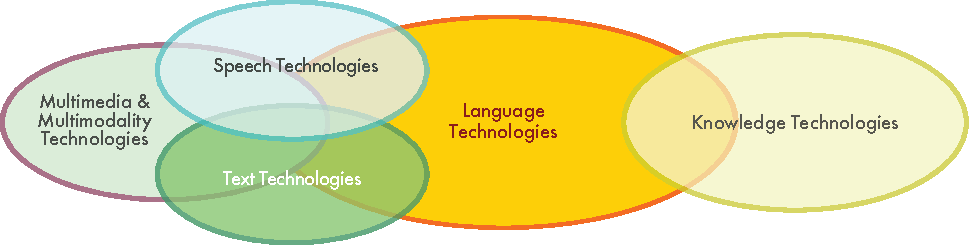
\includegraphics[width=\textwidth]{../_media/english/language_technologies}
  \caption{Language technology in context}
  \label{fig:ltincontext_en}
  \colorrule{grey3}{\textwidth}{1.5pt}
\end{figure*}

When we communicate, we combine language with other modes of communication and information media -- for example speaking can involve gestures and facial expressions. Digital texts link to pictures and sounds. Movies may contain language in spoken and written form. In other words, speech and text technologies overlap and interact with other multimodal communication and multimedia technologies.\\ 
In this section, we will discuss the main application areas of language technology, i.\,e., language checking, web search, speech interaction, and machine translation. These applications and basic technologies include 

\begin{itemize}
\item spelling correction
\item authoring support
\item computer-assisted language learning
\item information retrieval 
\item information extraction
\item text summarisation
\item question answering
\item speech recognition 
\item speech synthesis 
\end{itemize}

Language technology is an established area of research with an extensive set of introductory literature. The interested reader is referred to the following references:  \cite{carstensen-etal1, jurafsky-martin01, manning-schuetze1, lt-world1, lt-survey1}.

Before discussing the above application areas, we will briefly describe the architecture of a typical LT system.

\subsection{Application Architectures}

Software applications for language processing typically consist of several components that mirror different aspects of language. While such applications are typically very complex, figure~\ref{fig:textprocessingarch_en} shows a highly simplified architecture of a typical text processing system. The first three modules handle the structure and meaning of the text input:

\begin{enumerate}
\item Pre-processing: cleans the data, analyses or removes formatting, detects the input languages, and so on.
\item Grammatical analysis: finds the verb, its objects, modifiers and other parts of speech; detects the sentence structure.
\item Semantic analysis: performs disambiguation (i.\,e., computes the appropriate meaning of words in a given context); resolves anaphora (i.\,e., which pronouns refer to which nouns in the sentence); represents the meaning of the sentence in a machine-readable way.
\end{enumerate}

After analysing the text, task-specific modules can perform other operations, such as automatic summarisation and database look-ups.

In the remainder of this section, we firstly introduce the core application areas for language technology, and follow this with a brief overview of the state of LT research and education today, and a description of past and present research programmes. Finally, we present an expert estimate of core LT tools and resources for Icelandic in terms of various dimensions such as availability, maturity and quality. The general situation of LT for the Icelandic language is summarised in a matrix (figure~\ref{fig:lrlttable_en}). Tools and resources that are boldfaced in the text can also be found in figure~\ref{fig:lrlttable_en} (p.~\pageref{fig:lrlttable_en}) at the end of this chapter. LT support for Icelandic is also compared to other languages that are part of this series.

\begin{figure*}[htb]
  \colorrule{grey3}{\textwidth}{1.5pt}
  \center
  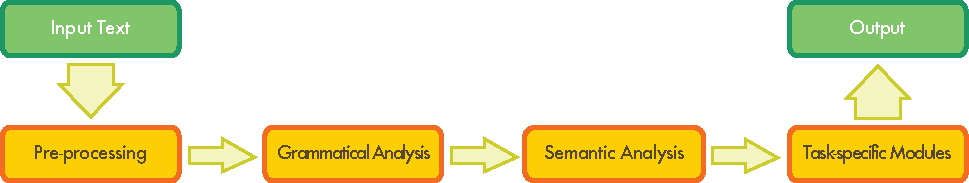
\includegraphics[width=\textwidth]{../_media/english/text_processing_app_architecture}
  \caption{A typical text processing architecture}
  \label{fig:textprocessingarch_en}
  \colorrule{grey3}{\textwidth}{1.5pt}
\end{figure*}

\subsection{Core Application Areas}

In this section, we focus on the most important LT tools and resources, and provide an overview of LT activities in Iceland. 

\subsubsection{Language Checking}

Anyone who has used a word processor such as Microsoft Word knows that it has a spell checker that highlights spelling mistakes and proposes corrections. The first spelling correction programs compared a list of extracted words against a dictionary of correctly spelled words. Today these programs are far more sophisticated. Using language-dependent algorithms for \textbf{grammatical analysis}, they detect errors related to morphology (e.\,g., plural formation) as well as syntax--related errors, such as a missing verb or a conflict of verb-subject agreement (e.\,g., \textit{she *write a letter}). However, most spell checkers will not find any errors in the following text \cite{zar1}:

\begin{quote}
  I have a spelling checker,\\
  It came with my PC.\\
  It plane lee marks four my revue\\
  Miss steaks aye can knot sea.
\end{quote}

Handling these kinds of errors usually requires an analysis of the context. For example: deciding if an Icelandic adjective should be written with a single (feminine) or double (masculine) ‘n’, as in

\begin{itemize}
\item Hann er \textbf{farinn}.
\item {[}He is gone.{]} 
\item Hún er \textbf{farin}.
\item {[}She is gone.{]}
\end{itemize}

This type of analysis either needs to draw on language-specific \textbf{grammars} laboriously coded into the software by experts, or on a statistical language model. In this case, a model calculates the probability of a particular word as it occurs in a specific position (e.\,g., between the words that precede and follow it). For example: \textit{Hann er farinn} is a probable word sequence whereas \textit{Hún er farin} is not. A statistical language model can be automatically created by using a large amount of (correct) language data, a \textbf{text corpus}. Most of these two approaches have been developed around data from English. Neither approach can transfer easily to Icelandic because the language has a flexible word order, unlimited compound building and a richer inflection system.

\begin{figure*}[htb]
  \colorrule{grey3}{\textwidth}{1.5pt}
  \center
  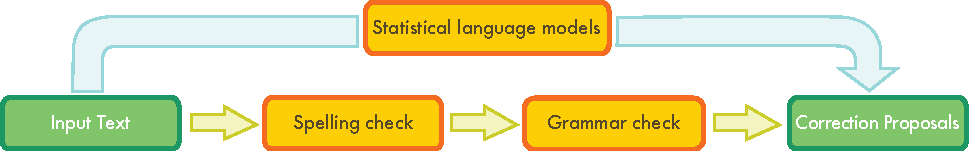
\includegraphics[width=\textwidth]{../_media/english/language_checking}
  \caption{Language checking (statistical; rule-based)}
  \label{fig:langcheckingaarch_en}
  \colorrule{grey3}{\textwidth}{1.5pt}
\end{figure*}

Language checking is not limited to word processors; it is also used in “authoring support systems”, i.\,e., software environments in which manuals and other types of technical documentation for complex IT, healthcare, engineering and other products, are written. To offset customer complaints about incorrect use and damage claims resulting from poorly understood instructions, companies are increasingly focusing on the quality of technical documentation while targeting the international market (via translation or localisation) at the same time. Advances in natural language processing have led to the development of authoring support software, which helps the writer of technical documentation to use vocabulary and sentence structures that are consistent with industry rules and (corporate) terminology restrictions.
\boxtext{The use of language checking is not limited to word processors. It also applies to authoring support systems.}
A spell checker for Icelandic has been available since Frisk Software developed the spell-checking program \textit{Púki} in the late 1980s. Since then the program has been improved and updated. It is available for MS Office and is widely used. Other spell checkers have also been developed. In 2002, the Dutch company Polderland developed a spell-checking program for the MS Office package. An open source spell checker for Icelandic also exists, that can be used with GNU/Linux applications and is based on Aspell. These programs are word-based, and hence cannot cope with many common spelling errors. A prototype of a context-sensitive spell checker has been integrated into LanguageTool\cite{lto1} and works with OpenOffice. This spell checker could possibly lay ground for a basic grammar checker, although no such tool exists for Icelandic.

    Besides spell checkers and authoring support, language checking is also important in the field of computer-assisted language learning. And language checking applications also automatically correct search engine queries, as found in Google's \textit{Did you mean…} suggestions.

\subsubsection{Web Search}

\begin{figure*}[htb]
  \colorrule{grey3}{\textwidth}{1.5pt}
  \center
  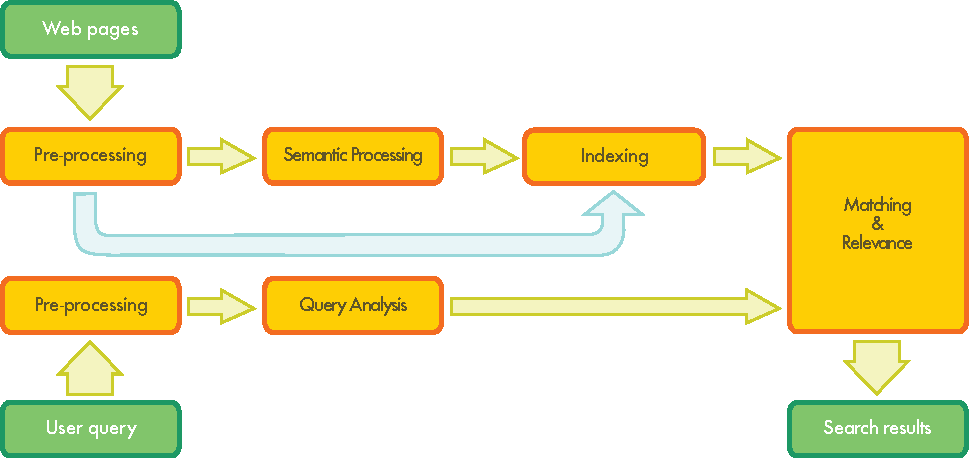
\includegraphics[width=\textwidth]{../_media/english/web_search_architecture}
  \caption{Web search}
  \label{fig:websearcharch_en}
  \colorrule{grey3}{\textwidth}{1.5pt}
 \end{figure*}

Searching the Web, intranets or digital libraries is probably the most widely used yet largely underdeveloped language technology application today. The Google search engine, which started in 1998, now handles about 80\% of all search queries \cite{spi1}. Since 2004, the verb \textit{gúg(g)la} is commonly used in Icelandic, even though it has not made its way into printed dictionaries.  The Google search interface and results page display has not significantly changed since the first version. However, in the current version, Google offers spelling correction for misspelled words and incorporates basic semantic search capabilities that can improve search accuracy by analysing the meaning of terms in a search query context \cite{pc1}. The Google success story shows that a large volume of data and efficient indexing techniques can deliver satisfactory results using a statistical approach to language processing. 

For more sophisticated information requests, it is essential to integrate deeper linguistic knowledge to facilitate text interpretation. Experiments using \textbf{lexical resources} such as machine-readable thesauri or ontological language resources (e.\,g., WordNet for English or GermaNet for German) have demonstrated improvements in finding pages using synonyms of the original search terms, such as \textit{hagnaður} {[}profit{]}, \textit{arður} {[}dividend{]}, \textit{gróði} {[}profit{]} and \textit{ábati} {[}gain{]}, or even more loosely related terms.
\boxtext{The next generation of search engines will have to include much more sophisticated language technology.}
The next generation of search engines will have to include much more sophisticated language technology, escpecially to deal with search queries consisting of a question or other sentence type rather than a list of keywords. For the query, \textit{Give me a list of all companies that were taken over by other companies in the last five years}, a syntactic as well as \textbf{semantic analysis} is required. The system also needs to provide an index to quickly retrieve relevant documents. A satisfactory answer will require syntactic parsing to analyse the grammatical structure of the sentence and determine that the user wants companies that have been acquired, rather than companies that have acquired other companies. For the expression \textit{last five years}, the system needs to determine the relevant range of years, taking into account the present year. The query then needs to be matched against a huge amount of unstructured data to find the pieces of information that are relevant to the user’s request. This process is called information retrieval, and involves searching and ranking relevant documents. To generate a list of companies, the system also needs to recognise a particular string of words in a document represents a company name, using a process called named entity recognition.

A more demanding challenge is matching a query in one language with documents in another language. Cross-lingual information retrieval involves automatically translating the query into all possible source languages and then translating the results back into the user's target language.

Now that data is increasingly found in non-textual formats, there is a need for services that deliver multimedia information retrieval by searching images, audio files and video data. In the case of audio and video files, a speech recognition module must convert the speech content into text (or into a phonetic representation) that can then be matched against a user query.

For inflectional languages like Icelandic, it is important to be able to search for all the inflectional forms of a word at once, instead of having to enter each different form separately. This can be done with the aid of a comprehensive full form database of modern Icelandic inflections, \textit{BÍN}\cite{bin1}, which has been developed at the Árni Magnússon Institute for Icelandic Studies. The database contains about 280,000 paradigms, with over 5.8 million inflectional forms. Each entry contains lemma, the word form, the word class and morphological features, for common nouns, proper nouns, adjectives, verbs, and adverbs.

A few years ago, the private company Spurl developed a search engine, \textit{Embla}, which made use of the database. The same algorithm is used for search in the Icelandic telephone directory and a few other sites. A similar feature, albeit not as sophisticated, has now been integrated into Google. At present, there is no large scale Icelandic language search engine project/product aside from Google’s Icelandic interface.

\subsubsection{Speech Interaction}

Speech interaction is one of many application areas that depend on speech technology, i.\,e., technologies for processing spoken language. Speech interaction technology is used to create interfaces that enable users to interact in spoken language instead of using a graphical display, keyboard and mouse.  Today, these voice user interfaces (VUI) are used for partially or fully automated telephone services provided by companies to customers, employees or partners. Business domains that rely heavily on VUIs include banking, supply chain, public transportation, and telecommunications. Other uses of speech interaction technology include interfaces to car navigation systems and the use of spoken language as an alternative to the graphical or touchscreen interfaces in smartphones.

\begin{figure*}[htb]
  \colorrule{grey3}{\textwidth}{1.5pt}
  \center
  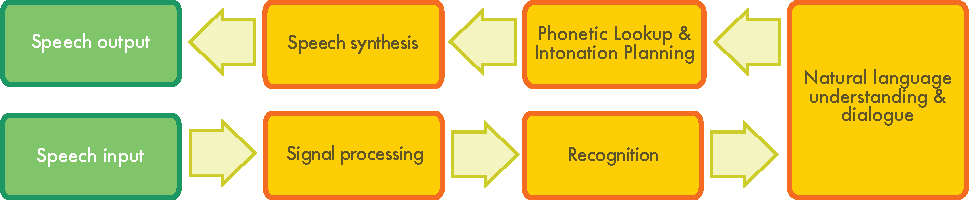
\includegraphics[width=\textwidth]{../_media/english/simple_speech-based_dialogue_architecture}
  \caption{Speech-based dialogue system}
  \label{fig:dialoguearch_en}
  \colorrule{grey3}{\textwidth}{1.5pt}
\end{figure*}

Speech interaction technology comprises four technologies: 

\begin{enumerate}
\item Automatic \textbf{speech recognition} (ASR) determines which words are actually spoken in a given sequence of sounds uttered by a user.  
\item Natural language understanding analyses the syntactic structure of a user’s utterance and interprets it according to the system in question.
\item Dialogue management determines which action to take given the user input and system functionality.   
\item \textbf{Speech synthesis} (text-to-speech or TTS) transforms the system’s reply into sounds for the user.
\end{enumerate}

One of the major challenges of ASR systems is to accurately recognise the words a user utters. This means restricting the range of possible user utterances to a limited set of keywords, or manually creating language models that cover a large range of natural language utterances. Using machine learning techniques, language models can also be generated automatically from \textbf{speech corpora}, i.\,e., large collections of speech audio files and text transcriptions. Restricting utterances usually forces people to use the voice user interface in a rigid way and can damage user acceptance; but the creation, tuning and maintenance of rich language models will significantly increase costs. VUIs that employ language models and initially allow a user to express their intent more flexibly — prompted by a \textit{How may I help you?} greeting — tend to be automated and are better accepted by users.
\boxtext{Speech interaction is the basis for creating interfaces that allow a user to interact with spoken language instead of a graphical dis-play, keyboard and mouse.}
Companies tend to use pre-recorded utterances by professional speakers for generating the output of the voice user interface. For static utterances where the wording does not depend on particular contexts of use or personal user data, this can deliver a rich user experience. But more dynamic content in an utterance may suffer from unnatural intonation because bits of audio files have simply been strung together. Through optimisation, today’s TTS systems are getting better at producing natural-sounding dynamic utterances.

Interfaces in speech interaction have been considerably standardised during the last decade in terms of their various technological components. There has also been strong market consolidation in speech recognition and speech synthesis. The national markets in the G20 countries (economically resilient countries with high populations) have been dominated by just five global players, with Nuance (USA) and Loquendo (Italy) being the most prominent players in Europe. In 2011, Nuance announced the acquisition of Loquendo, which represents a further step in market consolidation.

Two speech synthesisers have been developed for Icelandic. A formant-based speech synthesiser was originally made around 1990. This synthesiser was used mostly by the blind and visually impaired, while its quality was far from satisfactory for use in commercial applications for the general public.

In 2005, a new text-to-speech system was made under cooperation between the University of Iceland, Iceland Telecom and Hex Software. The system was trained by Nuance and uses their technology. This system has been used in commercial applications to some extent, but many users do not find its voice quality satisfactory. As the existing TTS systems are lacking in quality to their main users, the Icelandic Organisation of Blind and Partially Sighted is now planning to develop a new TTS system in cooperation with the University of Iceland, Reykjavik University, and the Polish Ivona software company. If everything goes as planned, this system will be ready in 2012\cite{tal1}. 

An isolated word speech recogniser for Icelandic was developed in 2003. The performance turned out to be quite satisfying, or at least 97\% word accuracy. An Icelandic student at the Tokyo Institute of Technology has developed a prototype of a system for automatic continuous speech recognition for Icelandic. This system reached up to 67.5\% word accuracy\cite{hind1}. Neither of these systems has been put to use in commercial applications. In the middle of 2011, Reykjavik University and the Icelandic Centre for Language Technology started cooperating with Google on preparatory work for developing a speech recogniser for Icelandic\cite{alm1}.

Looking ahead, there will be significant changes, due to the spread of smartphones as a new platform for managing customer relationships, in addition to fixed telephones, the Internet and e-mail. This will also affect how speech interaction technology is used. In the long term, there will be fewer telephone-based VUIs, and spoken language apps will play a far more central role as a user-friendly input for smartphones. This will be largely driven by stepwise improvements in the accuracy of speaker-independent speech recognition via the speech dictation services already offered as centralised services to smartphone users.

\subsubsection{Machine Translation}

\begin{figure*}[htb]
  \colorrule{grey3}{\textwidth}{1.5pt}
  \center
  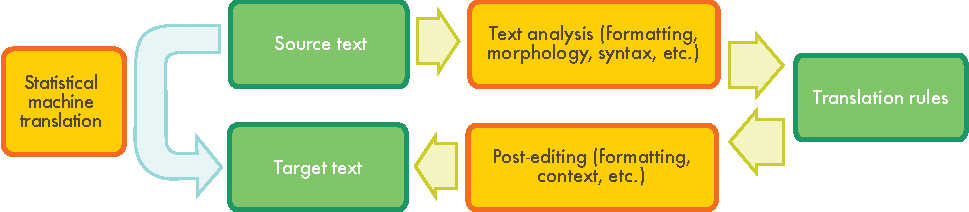
\includegraphics[width=\textwidth]{../_media/english/machine_translation}
  \caption{Machine translation (statistical; rule-based)}
  \label{fig:mtarch_en}
  \colorrule{grey3}{\textwidth}{1.5pt}
\end{figure*}

The idea of using digital computers to translate natural languages can be traced back to 1946 and was followed by substantial funding for research during the 1950s and again in the 1980s. 
Yet machine translation (MT) still cannot deliver on its initial promise of providing across-the-board automated translation.  
\boxtext{At its basic level, Machine Translation simply substitutes words in one natural language with words in another language.} Yet \textbf{machine translation} (MT) still cannot meet its initial promise of across-the-board automated translation. 

The most basic approach to machine translation is the automatic replacement of the words in a text written in one natural language with the equivalent words of another language. This can be useful in subject domains that have a very restricted, formulaic language such as weather reports.

However, in order to produce a good translation of less restricted texts, larger text units (phrases, sentences, or even whole passages) need to be matched to their closest counterparts in the target language. The major difficulty is that human language is ambiguous. Ambiguity creates challenges on multiple levels, such as word sense disambiguation on the lexical level (a \textit{jaguar} is a brand of car or an animal) or the assignment of case on the syntactic level, for example:

\begin{itemize}
\item Konan sá bílinn og \textbf{maðurinn hennar} líka.
\item Konan sá bílinn og \textbf{maðurinn hennar} líka.
\item The woman saw the car and her husband, too.
\end{itemize}

One way to build an MT system is to use linguistic rules. For translations between closely related languages, a translation using direct substitution may be feasible in cases such as the above example. However, rule-based (or linguistic knowledge-driven) systems often analyse the input text and create an intermediary symbolic representation from which the target language text can be generated. The success of these methods is highly dependent on the availability of extensive lexicons with morphological, syntactic, and semantic information, and large sets of grammar rules carefully designed by skilled linguists. This is a very long and therefore costly process.

In the late 1980s when computational power increased and became cheaper, interest in statistical models for machine translation began to grow. Statistical models are derived from analysing bilingual text corpora, \textbf{parallel corpora}, such as the Europarl parallel corpus, which contains the proceedings of the European Parliament in 11 European languages. Given enough data, statistical MT works well enough to derive an approximate meaning of a foreign language text by processing parallel versions and finding plausible patterns of words. Unlike knowledge-driven systems, however, statistical (or data-driven) MT systems often generate ungrammatical output. Data-driven MT is advantageous because less human effort is required, and it can also cover special particularities of the language (e.\,g., idiomatic expressions) that are often ignored in knowledge-driven systems. 

The strengths and weaknesses of knowledge-driven and data-driven machine translation tend to be complementary, so that nowadays researchers focus on hybrid approaches that combine both methodologies. One such approach uses both knowledge-driven and data-driven systems, together with a selection module that decides on the best output for each sentence. However, results for sentences longer than, say, 12 words, will often be far from perfect. A more effective solution is to combine the best parts of each sentence from multiple outputs; this can be fairly complex, as corresponding parts of multiple alternatives are not always obvious and need to be aligned. 
\boxtext{Machine Translation is particularly challenging for the Icelandic language.}
Machine translation is particularly challenging for the Icelandic language. The potential for creating arbitrary new words by compounding makes dictionary analysis and dictionary coverage difficult; free word order and split verb constructions pose problems for analysis; and extensive inflection is a challenge for generating words with proper markings for gender, case, number, mood, tense, etc.

The development in the area of MT for Icelandic has been limited. Stefán Briem, an independent researcher, has been engaged in MT since the early 1980s, resulting in his development of MT systems for Icelandic. In 2008 he launched a free web-based service, which offers translations between Icelandic and three other languages (English, Danish and Esperanto)\cite{tut1}. Hrafn Loftsson, a researcher at Reykjavik University, and his associates have been developing a rule-based shallow transfer translation system from Icelandic to English, based on the Apertium platform.\cite{ape1} A preliminary version is available online\cite{ape2}.  Google Translate has offered translations to and from Icelandic since 2009. The quality of the translations was rather poor in the beginning, but is getting better.

There is still a huge potential for improving the quality of MT systems. The challenges involve adapting language resources to a given subject domain or user area, and integrating the technology into workflows that already have term bases and translation memories. Another problem is that most of the current systems are English-centred and only support a few languages from and into Icelandic. This leads to friction in the translation workflow and forces MT users to learn different lexicon coding tools for different systems.

Evaluation campaigns help to compare the quality of MT systems, the different approaches and the status of the systems for different language pairs. Figure~\ref{fig:euromatrix_de} (p.~\pageref{fig:euromatrix_de}), which was prepared during the EC Euromatrix+ project, shows the pair-wise performances obtained for 22 of the 23 official EU languages (Irish was not compared). The results are ranked according to a BLEU score, which indicates higher scores for better translations \cite{bleu1}. A human translator would normally achieve a score of around 80 points.

The best results (in green and blue) were achieved by languages that benefit from a considerable research effort in coordinated programmes and the existence of many parallel corpora (e.\,g., English, French, Dutch, Spanish and German). The languages with poorer results are shown in red. These languages either lack such development efforts or are structurally very different from other languages (e.\,g., Hungarian, Maltese and Finnish).

\subsection{Other Application Areas}

Building language technology applications involves a range of subtasks that do not always surface at the level of interaction with the user, but they provide significant service functionalities “behind the scenes” of the system in question. They all form important research issues that have now evolved into individual sub-disciplines of computational linguistics.  Question answering, for example, is an active area of research for which annotated corpora have been built and scientific competitions have been initiated. The concept of question answering goes beyond keyword-based searches (in which the search engine responds by delivering a collection of potentially relevant documents) and enables users to ask a concrete question to which the system provides a single answer. For example:

\textit{Question: How old was Neil Armstrong when he stepped on the moon?}\\
\textit{Answer: 38.}

While question answering is obviously related to the core area of web search, it is nowadays an umbrella term for such research issues as which different types of questions exist, and how they should be handled; how a set of documents that potentially contain the answer can be analysed and compared (do they provide conflicting answers?); and how specific information (the answer) can be reliably extracted from a document without ignoring the context. 
\boxtext{Language technology applications often provide significant service functionalities "behind the scenes” of larger software systems.}
Question answering is in turn related to information extraction (IE), an area that was extremely popular and influential when computational linguistics took a statistical turn in the early 1990s. IE aims to identify specific pieces of information in specific classes of documents, such as the key players in company takeovers as reported in newspaper stories. Another common scenario that has been studied is reports on terrorist incidents. The task here consists of mapping appropriate parts of the text to a template that specifies the perpetrator, target, time, location and results of the incident. Domain-specific template-filling is the central characteristic of IE, which makes it another example of a “behind the scenes” technology that forms a well-demarcated research area, which in practice needs to be embedded into a suitable application environment. 

Text summarisation and \textbf{text generation} are two borderline areas that can act either as standalone applications or play a supporting role. Summarisation attempts to give the essentials of a long text in a short form, and is one of the features available in Microsoft Word. It mostly uses a statistical approach to identify the “important” words in a text (i.\,e., words that occur very frequently in the text in question but less frequently in general language use) and determine which sentences contain the most of these “important” words. These sentences are then extracted and put together to create the summary. In this very common commercial scenario, summarisation is simply a form of sentence extraction, and the text is reduced to a subset of its sentences. An alternative approach, for which some research has been carried out, is to generate brand new sentences that do not exist in the source text. 
\boxtext{For the Icelandic language, research in most text technologies is much less developed than for the English language.}
This requires a deeper understanding of the text, which means that so far this approach is far less robust. On the whole, a text generator is rarely used as a stand-alone application but is embedded into a larger software environment, such as a clinical information system that collects, stores and processes patient data. Creating reports is just one of many applications for text summarisation.

None of the technologies discussed in this section exist for Icelandic.

\subsection{Educational Programmes}

Language Technology is a highly interdisciplinary field, involving the expertise of linguists, computer scientists, mathematicians, philosophers, psycholinguists, and neuroscientists, among others. As such, it has not yet gained a firm ground in Icelandic higher education institutions. At the turn of the century, there were no programmes or even individual courses on Language Technology or Computational Linguistics at any Icelandic university or college, and there was no ongoing research in these areas.

In the fall of 2002, the University of Iceland launched an interdisciplinary Master’s programme in Language Technology. This is a two-year programme (120 ECTS credits), which admits students with either a B.A. degree in the humanities (languages and linguistics) or a B.Sc. degree in computer science (or electrical or software engineering). In 2007, the programme was relaunched, now as a joint programme between the Department of Icelandic at the University of Iceland and the School of Computer Science at Reykjavik University. During the operation period of the Nordic Graduate School of Language Technology (NGSLT) from 2004-2009 students could also take individual courses at other Nordic and Baltic universities.

Due to lack of resources, both financial and human, it has not been possible to enrol any new students in the Master’s programme since 2009. However, individual courses on Language Technology, Natural Language Processing and Corpus Linguistics are routinely offered at both the University of Iceland and Reykjavik University.

\subsection{National Projects and Initiatives}

There are only about 330,000 people speaking Icelandic, and this is not enough to sustain costly development of new products. It costs just as much to build language resources for Icelandic as for languages with hundreds of millions of speakers. As a result, the number of commercial companies in the language technology industry in Iceland is close to zero. Frisk Software has developed and sells the spell-checking program \textit{Púki}, but does not work on any new products. In the last decade, the companies Iceland Telecom and Hex Software worked with the University of Iceland in developing both an individual word speech recogniser and a text-to-speech system for Icelandic. Neither of these companies works on language or speech technology any longer.

Clara, a recent start-up company, provides service to companies that want to know what people think of their products and services. Clara’s system uses semantic analysis and data presentation methods to analyse the attitudes online. Their tool for analysing Icelandic language websites is called \textit{Vaktarinn}\cite{vak1}.  In its first year it had over 1200 users, counting non-paying trial users. Clara is the only company in Iceland currently developing revenue-generating LT products.

In 2000, the Icelandic Government launched a special Language Technology Programme with the aim of supporting institutions and companies in creating basic resources for Icelandic language technology. This initiative resulted in several projects which have had profound influence on the field in Iceland. The main direct products of the LT Programme are the following\cite{ilrt1}: 

\begin{itemize}
\item A full-form morphological database of Modern Icelandic inflections
\item A balanced morphosyntactically tagged corpus of 25 million words
\item A training model for data-driven PoS taggers
\item A text-to-speech system
\item An isolated word speech recogniser
\item An improved spell checker
\end{itemize}

After the Language Technology Programme ended in 2004, researchers from three institutes (University of Iceland, Reykjavik University, and the Árni Magnússon Institute for Icelandic Studies), who had been involved in most of the projects funded by the programme, decided to join forces in a consortium called the Icelandic Centre for Language Technology (ICLT), in order to follow up on the tasks of the programme. The main roles of the ICLT are to

\begin{itemize}
\item serve as an information centre on Icelandic LT by running a website (http://iclt.is); 
\item encourage cooperation on LT projects between universities, institutions and commercial companies;
\item organise and coordinate university education in LT;
\item participate in Nordic, Europeaan and international cooperation on LT;
\item initiate and participate in R\&D projects in LT;
\item keep track of resources and products in the field of Icelandic LT;
\item organise LT conferences for researchers, companies and the public;
\item support the growth of Icelandic LT in all possible manners.
\end{itemize}

Since 2005, the ICLT researchers have initiated several new projects which have been partly supported by the Icelandic Research Fund and the Icelandic Technical Development Fund. The most important product of these projects is the open source IceNLP package (IceTagger, IceParser and Lemmald)\cite{icenlp1} which is also available as an online service (http://nlp.cs.ru.is). In 2009, the ICLT received a relatively large three year Grant of Excellence from the Icelandic Research Fund to the project ‘Viable Language Technology beyond English -- Icelandic as a test case’. Within that project, further basic LT resources for Icelandic are being developed.

As we have seen, previous programmes have led to the development of a number of LT tools and resources for the Icelandic language. In the following section, the current state of LT support for Icelandic is summarised.
  
\subsection{Availability of Tools and Resources}

Figure~\ref{fig:lrlttable_en} provides a rating for language technology support for the Icelandic language. This rating of existing tools and resources was generated by leading experts in the field who provided estimates based on a scale from 0 (very low) to 6 (very high) using seven criteria.

\begin{figure*}[htb]
\centering
%\begin{tabular}{>{\columncolor{orange1}}p{.33\linewidth}ccccccc} % ORIGINAL
\begin{tabular}{>{\columncolor{orange1}}p{.33\linewidth}@{\hspace*{6mm}}c@{\hspace*{6mm}}c@{\hspace*{6mm}}c@{\hspace*{6mm}}c@{\hspace*{6mm}}c@{\hspace*{6mm}}c@{\hspace*{6mm}}c}
\rowcolor{orange1}
 \cellcolor{white}&\begin{sideways}\makecell[l]{Quantity}\end{sideways}
&\begin{sideways}\makecell[l]{\makecell[l]{Availability} }\end{sideways} &\begin{sideways}\makecell[l]{Quality}\end{sideways}
&\begin{sideways}\makecell[l]{Coverage}\end{sideways} &\begin{sideways}\makecell[l]{Maturity}\end{sideways} &\begin{sideways}\makecell[l]{Sustainability}\end{sideways} &\begin{sideways}\makecell[l]{Adaptability}\end{sideways} \\ \addlinespace
\multicolumn{8}{>{\columncolor{orange2}}l}{Language Technology: Tools, Technologies and Applications} \\ \addlinespace
Speech Recognition &1&1&1&1.5&1&0&1 \\ \addlinespace
Speech Synthesis &1&1&2.5&2.5&2&1&1\\ \addlinespace
Grammatical analysis &2&5.5&4&3&3.5&3.5&3\\ \addlinespace
Semantic analysis &0.5&0.5&0.5&0.5&0.5&0.5&0.5\\ \addlinespace
Text generation &0&0&0&0&0&0&0\\ \addlinespace
Machine translation &1&4&1&1.5&1.5&1.5&2\\ \addlinespace
\multicolumn{8}{>{\columncolor{orange2}}l}{Language Resources: Resources, Data and Knowledge Bases} \\ \addlinespace
Text corpora &1.5&4&3&2.5&2.5&4.5&3\\ \addlinespace
Speech corpora &1&2&1.5&1.5&1&1.5&1.5\\ \addlinespace
Parallel corpora &1&1&1&0.5&1&1&1\\ \addlinespace
Lexical resources &1&2&2.5&2.5&2&2&2\\ \addlinespace
Grammars &1&4&2.5&2&2.5&2.5&2\\
\end{tabular}
\caption{State of language technology support for Icelandic}
\label{fig:lrlttable_en}
\end{figure*}

The key results for Icelandic language technology can be summed up as follows:

\begin{itemize}
\item Icelandic stands reasonably well with respect to the most basic language technology tools and resources, such as text analysis and text corpora.
\item There exist also individual products with limited functionality in fields such as speech synthesis, speech recognition and machine translation, speech corpora, parallel corpora, and lexical resources. 
\item However, tools and resources for more advanced language technology such as text interpretation and language generation, simply do not exist.
\end{itemize}

At the end of the 20th century, Icelandic Language Technology was virtually non-existent. Things started to change in 1999, after a specially appointed Expert Group delivered a whitepaper on Language Technology to the Minister of Education, Science and Culture\cite{sky1}.  In this whitepaper, several actions to establish Icelandic Language Technology were proposed. The expert group estimated that it would cost around one billion Icelandic krónas (which then amounted to about ten million Euros) to make Icelandic LT self-sustained. After that, the free market should be able to take over, since it would have access to public resources that would have been created by the government-funded Language Technology Programme, and that would be made available on an equal basis to everyone who was going to use these resources in their commercial products.

It must be pointed out that the total budget of the Language Technology Programme from 2000-2004 was only around 1/8 of the sum that the expert group estimated would be needed\cite{ilrt1}.  It should therefore come as no surprise that Icelandic LT is still in its infancy. 330,000 speakers are simply to few to sustain costly development of new products. At present, almost no companies are working in the LT area because they do not see it as profitable. It is thus extremely important to continue public support for Icelandic LT for some time, but given the current financial situation, it does not seem likely that such support will be coming from the state budget any time soon.

\subsection{Cross-language comparison}

\begin{figure*}[tb]
  \small
  \centering
  \begin{tabular}
  { % defines color for each column.
  >{\columncolor{corange5}}p{.13\linewidth}@{\hspace{.040\linewidth}}
  >{\columncolor{corange4}}p{.13\linewidth}@{\hspace{.040\linewidth}}
  >{\columncolor{corange3}}p{.13\linewidth}@{\hspace{.040\linewidth}}
  >{\columncolor{corange2}}p{.13\linewidth}@{\hspace{.040\linewidth}}
  >{\columncolor{corange1}}p{.13\linewidth} 
  }
  \multicolumn{1}{>{\columncolor{white}}c@{\hspace{.040\linewidth}}}{\textbf{Excellent}} & 
  \multicolumn{1}{@{}>{\columncolor{white}}c@{\hspace{.040\linewidth}}}{\textbf{Good}} &
  \multicolumn{1}{@{}>{\columncolor{white}}c@{\hspace{.040\linewidth}}}{\textbf{Moderate}} &
  \multicolumn{1}{@{}>{\columncolor{white}}c@{\hspace{.040\linewidth}}}{\textbf{Fragmentary}} &
  \multicolumn{1}{@{}>{\columncolor{white}}c}{\textbf{Weak/no}} \\ 
  \multicolumn{1}{>{\columncolor{white}}c@{\hspace{.040\linewidth}}}{\textbf{support}} & 
  \multicolumn{1}{@{}>{\columncolor{white}}c@{\hspace{.040\linewidth}}}{\textbf{support}} &
  \multicolumn{1}{@{}>{\columncolor{white}}c@{\hspace{.040\linewidth}}}{\textbf{support}} &
  \multicolumn{1}{@{}>{\columncolor{white}}c@{\hspace{.040\linewidth}}}{\textbf{support}} &
  \multicolumn{1}{@{}>{\columncolor{white}}c}{\textbf{support}} \\ \addlinespace
  
& \vspace*{0.5mm}English
& \vspace*{0.5mm}
Czech \newline 
Dutch \newline 
Finnish \newline 
French \newline 
German \newline   
Italian \newline  
Portuguese \newline 
Spanish \newline
& \vspace*{0.5mm}Basque \newline 
Bulgarian \newline 
Catalan \newline 
Danish \newline 
Estonian \newline 
Galician\newline 
Greek \newline  
Hungarian  \newline
Irish \newline  
Norwegian \newline 
Polish \newline 
Serbian \newline 
Slovak \newline 
Slovene \newline 
Swedish \newline
& \vspace*{0.5mm}
Croatian \newline 
Icelandic \newline  
Latvian \newline 
Lithuanian \newline 
Maltese \newline 
Romanian\\
\end{tabular}
\caption{Speech processing: state of language technology support for 30 European languages}
\label{fig:speech_cluster_en}
\end{figure*}

\begin{figure*}[tb]
  \small
  \centering
  \begin{tabular}
  { % defines color for each column.
  >{\columncolor{corange5}}p{.13\linewidth}@{\hspace{.040\linewidth}}
  >{\columncolor{corange4}}p{.13\linewidth}@{\hspace{.040\linewidth}}
  >{\columncolor{corange3}}p{.13\linewidth}@{\hspace{.040\linewidth}}
  >{\columncolor{corange2}}p{.13\linewidth}@{\hspace{.040\linewidth}}
  >{\columncolor{corange1}}p{.13\linewidth} 
  }
  \multicolumn{1}{>{\columncolor{white}}c@{\hspace{.040\linewidth}}}{\textbf{Excellent}} & 
  \multicolumn{1}{@{}>{\columncolor{white}}c@{\hspace{.040\linewidth}}}{\textbf{Good}} &
  \multicolumn{1}{@{}>{\columncolor{white}}c@{\hspace{.040\linewidth}}}{\textbf{Moderate}} &
  \multicolumn{1}{@{}>{\columncolor{white}}c@{\hspace{.040\linewidth}}}{\textbf{Fragmentary}} &
  \multicolumn{1}{@{}>{\columncolor{white}}c}{\textbf{Weak/no}} \\ 
  \multicolumn{1}{>{\columncolor{white}}c@{\hspace{.040\linewidth}}}{\textbf{support}} & 
  \multicolumn{1}{@{}>{\columncolor{white}}c@{\hspace{.040\linewidth}}}{\textbf{support}} &
  \multicolumn{1}{@{}>{\columncolor{white}}c@{\hspace{.040\linewidth}}}{\textbf{support}} &
  \multicolumn{1}{@{}>{\columncolor{white}}c@{\hspace{.040\linewidth}}}{\textbf{support}} &
  \multicolumn{1}{@{}>{\columncolor{white}}c}{\textbf{support}} \\ \addlinespace
  
& \vspace*{0.5mm} English 
& \vspace*{0.5mm} 
French \newline 
Spanish
& \vspace*{0.5mm}
Catalan \newline 
Dutch \newline 
German \newline 
Hungarian \newline
Italian \newline 
Polish \newline 
Romanian \newline 
& \vspace*{0.5mm}Basque \newline 
Bulgarian \newline 
Croatian \newline 
Czech \newline
Danish \newline 
Estonian \newline 
Finnish \newline 
Galician \newline 
Greek \newline 
Icelandic \newline 
Irish \newline 
Latvian \newline 
Lithuanian \newline 
Maltese \newline 
Norwegian \newline 
Portuguese \newline 
Serbian \newline 
Slovak \newline 
Slovene \newline 
Swedish \newline 
\end{tabular}
\caption{Machine translation: state of language technology support for 30 European languages}
\label{fig:mt_cluster_en}
\end{figure*}

\begin{figure*}[tb]
  \small
  \centering
  \begin{tabular}
  { % defines color for each column.
  >{\columncolor{corange5}}p{.13\linewidth}@{\hspace{.040\linewidth}}
  >{\columncolor{corange4}}p{.13\linewidth}@{\hspace{.040\linewidth}}
  >{\columncolor{corange3}}p{.13\linewidth}@{\hspace{.040\linewidth}}
  >{\columncolor{corange2}}p{.13\linewidth}@{\hspace{.040\linewidth}}
  >{\columncolor{corange1}}p{.13\linewidth} 
  }
  \multicolumn{1}{>{\columncolor{white}}c@{\hspace{.040\linewidth}}}{\textbf{Excellent}} & 
  \multicolumn{1}{@{}>{\columncolor{white}}c@{\hspace{.040\linewidth}}}{\textbf{Good}} &
  \multicolumn{1}{@{}>{\columncolor{white}}c@{\hspace{.040\linewidth}}}{\textbf{Moderate}} &
  \multicolumn{1}{@{}>{\columncolor{white}}c@{\hspace{.040\linewidth}}}{\textbf{Fragmentary}} &
  \multicolumn{1}{@{}>{\columncolor{white}}c}{\textbf{Weak/no}} \\ 
  \multicolumn{1}{>{\columncolor{white}}c@{\hspace{.040\linewidth}}}{\textbf{support}} & 
  \multicolumn{1}{@{}>{\columncolor{white}}c@{\hspace{.040\linewidth}}}{\textbf{support}} &
  \multicolumn{1}{@{}>{\columncolor{white}}c@{\hspace{.040\linewidth}}}{\textbf{support}} &
  \multicolumn{1}{@{}>{\columncolor{white}}c@{\hspace{.040\linewidth}}}{\textbf{support}} &
  \multicolumn{1}{@{}>{\columncolor{white}}c}{\textbf{support}} \\ \addlinespace

& \vspace*{0.5mm}English
& \vspace*{0.5mm}
  Dutch \newline 
  French \newline 
  German \newline 
  Italian \newline 
  Spanish
& \vspace*{0.5mm}Basque \newline 
  Bulgarian \newline 
  Catalan \newline 
  Czech \newline 
  Danish \newline 
  Finnish \newline 
  Galician \newline 
  Greek \newline 
  Hungarian \newline 
  Norwegian \newline 
  Polish \newline 
  Portuguese \newline 
  Romanian \newline 
  Slovak \newline 
  Slovene \newline 
  Swedish \newline 
& \vspace*{0.5mm}
  Croatian \newline 
  Estonian \newline 
  Icelandic \newline 
  Irish \newline 
  Latvian \newline 
  Lithuanian \newline 
  Maltese \newline 
  Serbian \\
  \end{tabular}
\caption{Text analysis: state of language technology support for 30 European languages}
\label{fig:text_cluster_en}
\end{figure*}

\begin{figure*}[tb]
  \small
  \centering
  \begin{tabular}
  { % defines color for each column.
  >{\columncolor{corange5}}p{.13\linewidth}@{\hspace{.040\linewidth}}
  >{\columncolor{corange4}}p{.13\linewidth}@{\hspace{.040\linewidth}}
  >{\columncolor{corange3}}p{.13\linewidth}@{\hspace{.040\linewidth}}
  >{\columncolor{corange2}}p{.13\linewidth}@{\hspace{.040\linewidth}}
  >{\columncolor{corange1}}p{.13\linewidth} 
  }
  \multicolumn{1}{>{\columncolor{white}}c@{\hspace{.040\linewidth}}}{\textbf{Excellent}} & 
  \multicolumn{1}{@{}>{\columncolor{white}}c@{\hspace{.040\linewidth}}}{\textbf{Good}} &
  \multicolumn{1}{@{}>{\columncolor{white}}c@{\hspace{.040\linewidth}}}{\textbf{Moderate}} &
  \multicolumn{1}{@{}>{\columncolor{white}}c@{\hspace{.040\linewidth}}}{\textbf{Fragmentary}} &
  \multicolumn{1}{@{}>{\columncolor{white}}c}{\textbf{Weak/no}} \\ 
  \multicolumn{1}{>{\columncolor{white}}c@{\hspace{.040\linewidth}}}{\textbf{support}} & 
  \multicolumn{1}{@{}>{\columncolor{white}}c@{\hspace{.040\linewidth}}}{\textbf{support}} &
  \multicolumn{1}{@{}>{\columncolor{white}}c@{\hspace{.040\linewidth}}}{\textbf{support}} &
  \multicolumn{1}{@{}>{\columncolor{white}}c@{\hspace{.040\linewidth}}}{\textbf{support}} &
  \multicolumn{1}{@{}>{\columncolor{white}}c}{\textbf{support}} \\ \addlinespace
    
& \vspace*{0.5mm}English
& \vspace*{0.5mm} 
    Czech \newline 
    Dutch \newline 
    French \newline 
    German \newline 
    Hungarian \newline
    Italian \newline
    Polish \newline
    Spanish \newline
    Swedish \newline 
& \vspace*{0.5mm} Basque\newline 
    Bulgarian\newline 
    Catalan \newline 
    Croatian \newline 
    Danish \newline 
    Estonian \newline 
    Finnish \newline 
    Galician \newline 
    Greek \newline 
    Norwegian \newline 
    Portuguese \newline 
    Romanian \newline 
    Serbian \newline 
    Slovak \newline 
    Slovene \newline
&  \vspace*{0.5mm}
    Icelandic \newline 
    Irish \newline 
    Latvian \newline 
    Lithuanian \newline 
    Maltese  \\
  \end{tabular}
  \caption{Speech and text resources: State of support for 30 European languages}  
  \label{fig:resources_cluster_en}
\end{figure*}

The current state of LT support varies considerably from one language community to another. In order to compare the situation between languages, this section will present an evaluation based on two sample application areas (machine translation and speech processing) and one underlying technology (text analysis), as well as basic resources needed for building LT applications. The languages were categorised using the following five-point scale: 

\begin{enumerate}
\item Excellent support
\item Good support
\item Moderate support
\item Fragmentary support
\item Weak or no support
\end{enumerate}

LT support was measured according to the following criteria:

\textbf{Speech Processing:} Quality of existing speech recognition technologies, quality of existing speech synthesis technologies, coverage of domains, number and size of existing speech corpora, amount and variety of available speech-based applications.

\textbf{Machine Translation:} Quality of existing MT technologies, number of language pairs covered, coverage of linguistic phenomena and domains, quality and size of existing parallel corpora, amount and variety of available MT applications.

\textbf{Text Analysis:} Quality and coverage of existing text analysis technologies (morphology, syntax, semantics), coverage of linguistic phenomena and domains, amount and variety of available applications, quality and size of existing (annotated) text corpora, quality and coverage of existing lexical resources (e.\,g., WordNet) and grammars.

\textbf{Resources:} Quality and size of existing text corpora, speech corpora and parallel corpora, quality and coverage of existing lexical resources and grammars.

Figures~\ref{fig:speech_cluster_en} to~\ref{fig:resources_cluster_en} show that Icelandic is in the bottom cluster for all of the tools and resources listed. It compares well with other languages with a small number of speakers, such as Irish, Latvian, Lithuanian, and Maltese. These languages lag far behind large languages like German and French, for instance. But even LT resources and tools for those languages clearly do not yet reach the quality and coverage of comparable resources and tools for the English language, which is in the lead in almost all LT areas. And there are still plenty of gaps in English language resources with regard to high quality applications.

\subsection{Conclusions}

\emph{In this series of white papers, we have made an important effort by assessing the language technology support for 30 European languages, and by providing a high-level comparison across these languages. By identifying the gaps, needs and deficits, the European language technology community and its related stakeholders are now in a position to design a large scale research and development programme aimed at building a truly multilingual, technology-enabled communication across Europe.}

The results of this white paper series show that there is a dramatic difference in language technology support for the various European languages. While there are good quality software and resources available for some languages and application areas, others, usually smaller languages, have substantial gaps. Many languages lack basic technologies for text analysis and the essential resources. Others have basic tools and resources but the implementation of for example semantic methods is still far away. Therefore a large-scale effort is needed to attain the ambitious goal of providing high-quality language technology support for all European languages, for example through high quality machine translation. 

For a small language community and a small research environment such as the Icelandic one, it is vital to cooperate, not only on the national level but also internationally. It is to be hoped that Iceland’s participation in META-NORD and META-NET will make it possible to develop, standardise and make available several important LT resources and thus contribute to the growth of Icelandic language technology.

The long term goal of META-NET is to enable the creation of high-quality language technology for all languages. This requires all stakeholders - in politics, research, business, and society - to unite their efforts. The resulting technology will help tear down existing barriers and build bridges between Europe’s languages, paving the way for political and economic unity through cultural diversity. 
\end{multicols}

\clearpage

\ssection[About META-NET]{About META-NET}

\begin{multicols}{2}
META-NET is a Network of Excellence funded by the European Commission. The network currently consists of 54 members from 33 European countries. META-NET fosters the Multilingual Europe Technology Alliance (META), a growing community of language technology professionals and organisations in Europe. META-NET cooperates with other initiatives like the Common Language Resources and Technology Infrastructure (CLARIN), which is helping establish digital humanities research in Europe. META-NET fosters the technological foundations for a truly multilingual European information society that:

\begin{itemize}
\item makes communication and cooperation possible across languages;
\item provides equal access to information and knowledge in any language;
\item offers advanced and affordable networked information technology to European citizens.
\end{itemize}

META-NET stimulates and promotes multilingual technologies for all European languages. The technologies enable automatic translation, content production, information processing and knowledge management for a wide variety of applications and subject domains. The network wants to improve current approaches, so better communication and cooperation across languages can take place. Europeans have an equal right to information and knowledge regardless of language.

META-NET launched on 1 February 2010 with the goal of advancing research in language technology (LT). The network supports a Europe that unites as a single digital market and information space. META-NET has conducted several activities that further its goals. META-VISION, META-SHARE and META-RESEARCH are the network’s three lines of action.

\textbf{META-VISION} fosters a dynamic and influential stakeholder community that unites around a shared vision and a common strategic research agenda (SRA). The main focus of this activity is to build a coherent and cohesive LT community in Europe by bringing together representatives from highly fragmented and diverse groups of stakeholders. In the first year of META-NET, presentations at the FLaReNet Forum (Spain), Language Technology Days (Luxembourg), JIAMCATT 2010 (Luxembourg), LREC 2010 (Malta), EAMT 2010 (France) and ICT 2010 (Belgium) centred on public outreach. According to initial estimates, META-NET has already contacted more than 2,500 LT professionals to develop its goals and visions with them. At the META-FORUM 2010 event in Brussels, META-NET communicated the initial results of its vision building process to more than 250 participants. In a series of interactive sessions, the participants provided feedback on the visions presented by the network. 

\textbf{META-SHARE} creates an open, distributed facility for exchanging and sharing resources. The peer-to-peer network of repositories will contain language data, tools and web services that are documented with high-quality metadata and organised in standardised categories. The resources can be readily accessed and uniformly searched. The available resources include free, open source materials as well as restricted, commercially available, fee-based items. META-SHARE targets existing language data, tools and systems as well as new and emerging products that are required for building and evaluating new technologies, products and services. The reuse, combination, repurposing and re-engineering of language data and tools plays a crucial role. META-SHARE will eventually become a critical part of the LT marketplace for developers, localisation experts, researchers, translators and language professionals from small, mid-sized and large enterprises. META-SHARE addresses the full development cycle of LT—from research to innovative products and services. A key aspect of this activity is establishing META-SHARE as an important and valuable part of a European and global infrastructure for the LT community. 

\textbf{META-RESEARCH} builds bridges to related technology fields. This activity seeks to leverage advances in other fields and to capitalise on innovative research that can benefit language technology. In particular, this activity wants to bring more semantics into machine translation (MT), optimise the division of labour in hybrid MT, exploit context when computing automatic translations and prepare an empirical base for MT. META-RESEARCH is working with other fields and disciplines, such as machine learning and the Semantic Web community. META-RESEARCH focuses on collecting data, preparing data sets and organising language resources for evaluation purposes; compiling inventories of tools and methods; and organising workshops and training events for members of the community. This activity has already clearly identified aspects of MT where semantics can impact current best practices. In addition, the activity has created recommendations on how to approach the problem of integrating semantic information in MT. META-RESEARCH is also finalising a new language resource for MT, the Annotated Hybrid Sample MT Corpus, which provides data for English-German, English-Spanish and English-Czech language pairs. META-RESEARCH has also developed software that collects multilingual corpora that are hidden on the Web.
\end{multicols}
\vfill
\centerline{office@meta-net.eu -- http://www.meta-net.eu}

\cleardoublepage

\appendix
\addtocontents{toc}{\protect\bigskip}

\bsection[Tilvísanir -- References]{Tilvísanir --- References}
\bibliographystyle{unsrt}
\bibliography{references_is}
  
\cleardoublepage

\bsection[META-NET þátttakendur -- META-NET Members]{META-NET þátttakendur --- META-NET Members}
\label{metanetmembers}

\small
\begin{longtable}{llp{105mm}}
  Austurríki & \textcolor{grey1}{Austria} & Zentrum für Translationswissenschaft, Universität Wien: Gerhard Budin\\ \addlinespace 
  Belgía & \textcolor{grey1}{Belgium} & Computational Linguistics and Psycholinguistics Research Centre, Univ. of Antwerp: Walter Daelemans\\ \addlinespace
  & & Centre for Proc. Speech and Images, Univ. of Leuven: Dirk van Compernolle \\ \addlinespace
  Bretland & \textcolor{grey1}{UK} & Inst. for Lang., Cognition and Computation, Center for Speech Technology Research, Univ. of Edinburgh: Steve Renals \\ \addlinespace 
  & & Research Inst. of Informatics and Lang. Proc., Univ. of Wolverhampton: Ruslan Mitkov \\ \addlinespace 
  & & School of Computer Science, Univ. of Manchester: Sophia Ananiandou \\ \addlinespace 
  Búlgaría & \textcolor{grey1}{Bulgaria} & Inst. for Bulgarian Lang., Bulgarian Academy of Sciences: Svetla Koeva \\ \addlinespace
  Danmörk &  \textcolor{grey1}{Denmark} & Centre for Lang. Technology, Univ. of Copenhagen: Bolette Sandford Pedersen, Bente Maegaard\\ \addlinespace
  Eistland & \textcolor{grey1}{Estonia} & Inst. of Computer Science, Univ. of Tartu: Tiit Roosmaa\\ \addlinespace
  Finnland & \textcolor{grey1}{Finland} & Computational Cognitive Systems Research Group, Aalto Univ.: Timo Honkela\\ \addlinespace
  & & Dept. of General Linguistics, Univ. of Helsinki: Kimmo Koskenniemi, Krister Linden \\ \addlinespace
  Frakkland & \textcolor{grey1}{France} & Centre National de la Recherche Scientifique, Laboratoire d'Informatique pour la Mécanique et les Sciences de l'Ingénieur: Joseph Mariani \\ \addlinespace
  & & Evaluations and Lang. Resources Distribution Agency: Khalid Choukri\\ \addlinespace 
  Grikkland & \textcolor{grey1}{Greece} & Inst. for Lang. and Speech Proc., R.C. “Athena”: Stelios Piperidis\\ \addlinespace 
  Holland & \textcolor{grey1}{Netherlands} & Utrecht Inst. of Linguistics, Utrecht Univ.: Jan Odijk\\ \addlinespace 
  & & Computational Linguistics, Univ. of Groningen: Gertjan van Noord\\ \addlinespace
  Írland & \textcolor{grey1}{Ireland} & School of Computing, Dublin City Univ.: Josef van Genabith\\ \addlinespace
  Ísland & \textcolor{grey1}{Iceland} & School of Humanities, Univ. of Iceland: Eiríkur Rögnvaldsson\\ \addlinespace
  Ítalía & \textcolor{grey1}{Italy} & Consiglio Nazionale Ricerche, Istituto di Linguistica Computazionale “Antonio Zampolli”: Nicoletta Calzolari\\ \addlinespace
  & & Human Lang. Technology, Fondazione Bruno Kessler: Bernardo Magnini\\ \addlinespace 
  Króatía & \textcolor{grey1}{Croatia} & Inst. of Linguistics, Faculty of Humanities and Social Science, Univ. of Zagreb: Marko Tadić \\ \addlinespace
  Kýpur & \textcolor{grey1}{Cyprus} & Lang. Centre, School of Humanities: Jack Burston\\ \addlinespace 
  Lettland & \textcolor{grey1}{Latvia} & Tilde: Andrejs Vasiljevs\\ \addlinespace 
  & & Inst. of Mathematics and Computer Science, Univ. of Latvia: Inguna Skadina\\ \addlinespace
  Litháen & \textcolor{grey1}{Lithuania} & Inst. of the Lithuanian Lang.: Jolanta Zabarskaitė\\ \addlinespace
  Lúxembúrg & \textcolor{grey1}{Luxembourg} & Arax Ltd.: Vartkes Goetcherian\\ \addlinespace
  Malta & \textcolor{grey1}{Malta} & Dept. Intelligent Computer Systems, Univ. of Malta: Mike Rosner\\ \addlinespace
  Noregur & \textcolor{grey1}{Norway} & Dept. of Linguistic, Univ. of Bergen: Koenraad De Smedt\\ \addlinespace 
  & & Dept. of Informatics, Lang. Technology Group, Univ. of Oslo: Stephan Oepen \\ \addlinespace
  Portúgal & \textcolor{grey1}{Portugal} & Dept. of Informatics, Univ. of Lisbon: Antonio Branco\\ \addlinespace
  & & Spoken Lang. Systems Lab., Inst. for Systems Engineering and Computers: Isabel Trancoso \\ \addlinespace
  Pólland & \textcolor{grey1}{Poland} & Inst. of Computer Science, Polish Academy of Sciences: Adam Przepiórkowski, Maciej Ogrodniczuk \\ \addlinespace
  & & Univ. of Łódź: Barbara Lewandowska-Tomaszczyk, Piotr Pęzik\\ \addlinespace
  & & Dept. of Computer Linguistics and Artificial Intelligence, Adam Mickiewicz Univ.: Zygmunt Vetulani \\ \addlinespace
  Rúmenía & \textcolor{grey1}{Romania} & Research Inst. for Artificial Intelligence, Romanian Academy of Sciences: Dan Tufis \\ \addlinespace
  & & Faculty of Computer Science, Univ. Alexandru Ioan Cuza: Dan Cristea \\ \addlinespace
  Serbía & \textcolor{grey1}{Serbia} & Faculty of Mathematics, Belgrade Univ.: Dusko Vitas, Cvetana Krstev, Ivan Obradovic \\ \addlinespace
  & & Pupin Inst.: Sanja Vranes \\ \addlinespace  
  Slóvakía & \textcolor{grey1}{Slovakia} & Ludovit Stur Inst. of Linguistics, Slovak Academy of Sciences: Radovan Garabik \\ \addlinespace 
  Slóvenía & \textcolor{grey1}{Slovenia} & Jozef Stefan Inst.: Marko Grobelnik \\ \addlinespace 
  Spánn & \textcolor{grey1}{Spain} & Barcelona Media: Toni Badia \\ \addlinespace 
  & & Institut Universitari de Lingüistica Aplicada, Univ. Pompeu Fabra: Núria Bel \\ \addlinespace 
  & & Aholab Signal Proc. Lab., Univ. of the Basque Country: Inma Hernaez Rioja \\ \addlinespace 
  & & Center for Lang. and Speech Technologies and Applications, Technical Univ. of Catalonia: Asunción Moreno \\ \addlinespace 
  & & Dept. of Signal Proc. and Communications, Univ. of Vigo: Carmen García Mateo \\ \addlinespace 
  Sviss & \textcolor{grey1}{Switzerland} & Idiap Research Inst.: Hervé Bourlard \\ \addlinespace 
  Svíþjóð & \textcolor{grey1}{Sweden} & Dept. of Swedish Lang., Univ. of Gothenburg: Lars Borin \\ \addlinespace 
  Tékkland & \textcolor{grey1}{Czech Republic} & Inst. of Formal and Applied Linguistics, Charles Univ. in Prague: Jan Hajic \\ \addlinespace
  Ungverjaland & \textcolor{grey1}{Hungary} & Research Inst. for Linguistics, Hungarian Academy of Sciences: Tamás Váradi\\  \addlinespace
  & & Dept. of Telecommunications and Media Informatics, Budapest Univ. of Technology and Economics: Géza Németh and Gábor Olaszy\\ \addlinespace
  Þýskaland & \textcolor{grey1}{Germany} & DFKI (German Research Centre for Artificial Intelligence): Hans Uszkoreit, Georg Rehm\\ \addlinespace
  & & Human Lang. Technology and Pattern Recognition, RWTH Aachen Univ.: Hermann Ney \\ \addlinespace
  & & Dept. of Computational Linguistics, Saarland Univ.: Manfred Pinkal
\end{longtable}
\normalsize

\renewcommand*{\figureformat}{}
\renewcommand*{\captionformat}{}

\begin{figure*}[htbp]
  \colorrule{grey3}{\textwidth}{1.5pt}
  \center
  %\fbox{-- META-NET group picture omitted to keep the size of the PDF file small. --}
  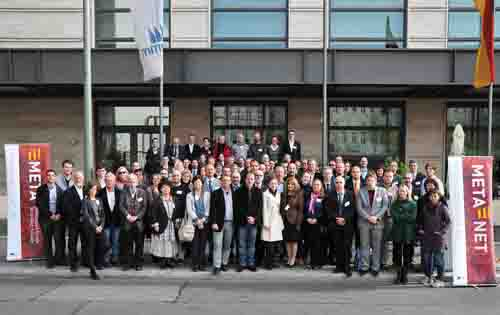
\includegraphics[width=\textwidth]{../_media/meta-net_team.jpg}
  \caption{Hátt í 100 sérfræðingar í máltækni -- fulltrúar þeirra landa og tungumála sem taka þátt í META-NET -- ræddu og samræmdu meginniðurstöður og ábendingar hvítbókanna á fundi META-NET í Berlín í Þýskalandi 21.-22. október 2011. --- \textcolor{grey1}{About 100 language technology experts -- representatives of the countries and languages represented in META-NET -- discussed and finalised the key results and messages of the White Paper Series at a META-NET meeting in Berlin, Germany, on October 21/22, 2011.}}
  \medskip
  \colorrule{grey3}{\textwidth}{1.5pt}
\end{figure*}


\cleardoublepage

\bsection[Hvítbókaröð META-NET -- The META-NET White Paper Series]{Hvítbókaröð META-NET --- The META-NET\ \ \ \ \ \ White Paper Series}
\label{whitepaperseries}

\vspace*{-5mm}
\centering
  \setlength{\tabcolsep}{2em}
  \begin{tabularx}{\textwidth}{lllll} \toprule\addlinespace
  %\begin{tabulary}{170mm}{LLL} \toprule
  &Baskneska & Basque & euskara& \\
  &Búlgarska & Bulgarian & български& \\
  &Danska & Danish & dansk& \\
  &Eistneska & Estonian & eesti& \\
  &Enska & English & English& \\
  &Finnska & Finnish & suomi& \\
  &Franska & French & français& \\
  &Galisíska & Galician & galego& \\
  &Gríska & Greek & ελληνικά& \\
  &Hollenska & Dutch & Nederlands& \\
  &Írska & Irish & Gaeilge& \\
  &Íslenska & Icelandic & íslenska& \\
  &Ítalska & Italian & italiano& \\
  &Katalónska & Catalan & català& \\
  &Króatíska & Croatian & hrvatski& \\
  &Lettneska & Latvian & latviešu valoda& \\
  &Litháíska & Lithuanian & lietuvių kalba& \\
  &Maltneska & Maltese & Malti& \\
  &Norska - bókmál & Norwegian Bokmål & bokmål& \\
  &Nýnorska & Norwegian Nynorsk & nynorsk& \\
  &Portúgalska & Portuguese & português& \\
  &Pólska & Polish & polski& \\
  &Rúmenska & Romanian & română& \\
  &Serbneska & Serbian & српски& \\
  &Slóvakíska & Slovak & slovenčina& \\
  &Slóvenska & Slovene & slovenščina& \\
  &Spænska & Spanish & español& \\
  &Sænska & Swedish & svenska& \\
  &Tékkneska & Czech & čeština& \\
  &Ungverska & Hungarian & magyar& \\
  &Þýska & German & Deutsch& \\  \bottomrule
\end{tabularx}

\end{document}
